\documentclass[11pt,a4paper,oneside]{report}             % Single-side
%\documentclass[11pt,a4paper,twoside,openright]{report}  % Duplex

% thanks to http://tex.stackexchange.com/a/47579/71109
\usepackage{ifxetex}
\usepackage{ifluatex}
\newif\ifxetexorluatex % a new conditional starts as false
\ifnum 0\ifxetex 1\fi\ifluatex 1\fi>0
   \xetexorluatextrue
\fi

\ifxetexorluatex
  \usepackage{fontspec}
\else
  \usepackage[T1]{fontenc}
  \usepackage[utf8]{inputenc}
  \usepackage[lighttt]{lmodern}
  \ttfamily\DeclareFontShape{T1}{lmtt}{m}{it}{<->sub*lmtt/m/sl}{}
\fi

\usepackage[english,magyar]{babel} % Alapértelmezés szerint utoljára definiált nyelv lesz aktív, de később külön beállítjuk az aktív nyelvet.

\usepackage{emptypage} % omit page number on empty pages

%\usepackage{cmap}
\usepackage{amsfonts,amsmath,amssymb} % Mathematical symbols.
%\usepackage[ruled,boxed,resetcount,linesnumbered]{algorithm2e} % For pseudocodes. % beware: this is not compatible with LuaLaTeX, see http://tex.stackexchange.com/questions/34814/lualatex-and-algorithm2e
\usepackage{booktabs} % For publication quality tables for LaTeX
\usepackage{graphicx}

%\usepackage{fancyhdr}
%\usepackage{lastpage}

\usepackage{geometry}
%\usepackage{sectsty}
\usepackage{setspace} % For setting line spacing

\usepackage[unicode]{hyperref} % For hyperlinks in the generated document.
\usepackage{xcolor}
\usepackage{listings} % For source code snippets.

\usepackage[amsmath,thmmarks]{ntheorem} % Theorem-like environments.

\usepackage[hang]{caption}

\singlespacing

\newcommand{\selecthungarian}{
	\selectlanguage{magyar}
	\setlength{\parindent}{2em}
	\setlength{\parskip}{0em}
	\frenchspacing
}

\newcommand{\selectenglish}{
	\selectlanguage{english}
	\setlength{\parindent}{0em}
	\setlength{\parskip}{0.5em}
	\nonfrenchspacing
	\renewcommand{\figureautorefname}{Figure}
	\renewcommand{\tableautorefname}{Table}
	\renewcommand{\partautorefname}{Part}
	\renewcommand{\chapterautorefname}{Chapter}
	\renewcommand{\sectionautorefname}{Section}
	\renewcommand{\subsectionautorefname}{Section}
	\renewcommand{\subsubsectionautorefname}{Section}
}

\usepackage[numbers]{natbib}
\usepackage{xspace}


%TODO Set the main variables
\newcommand{\vikszerzoVezeteknev}{Csernátony}
\newcommand{\vikszerzoKeresztnev}{Döme Máté}

\newcommand{\vikkonzulensAMegszolitas}{Dr.~}
\newcommand{\vikkonzulensAVezeteknev}{Vörös}
\newcommand{\vikkonzulensAKeresztnev}{András}

\newcommand{\vikcim}{Kiberfizikai rendszerek modellalapú kiberbiztonsági analízise} % Cím
\newcommand{\viktanszek}{\bmemit} % Tanszék
\newcommand{\vikdoktipus}{\msc} % Dokumentum típusa (\bsc vagy \msc)
\newcommand{\vikmunkatipusat}{diplomatervet} % a "hallgató nyilatkozat" részhez: szakdolgozatot vagy diplomatervet

%--------------------------------------------------------------------------------------
% TDK-specifikus változók
%--------------------------------------------------------------------------------------
\newcommand{\tdkszerzoB}{Második Szerző} % Második szerző neve; hagyd üresen, ha egyedül írtad a TDK-t.
\newcommand{\tdkev}{2014} % A dolgozat írásának éve (pl. "2014") (Ez OTDK-nál eltérhet az aktuális évtől.)

% További adatok az OTDK címlaphoz (BME-s TDK-hoz nem kell kitölteni)
\newcommand{\tdkevfolyamA}{IV} % Első szerző évfolyama, római számmal (pl. IV).
\newcommand{\tdkevfolyamB}{III} % Második szerző évfolyama, római számmal (pl. III).
\newcommand{\tdkkonzulensbeosztasA}{egyetemi tanár} % Első konzulens beosztása (pl. egyetemi docens)
\newcommand{\tdkkonzulensbeosztasB}{doktorandusz} % Második konzulens beosztása (pl. egyetemi docens)

\newcommand{\szerzoMeta}{\vikszerzoVezeteknev{} \vikszerzoKeresztnev} % egy szerző esetén
%\newcommand{\szerzoMeta}{\vikszerzoVezeteknev{} \vikszerzoKeresztnev, \tdkszerzoB} % két szerző esetén

%TODO Language configuration -- choose one
% Beállítások magyar nyelvű dolgozathoz
%--------------------------------------------------------------------------------------
% Elnevezések
%--------------------------------------------------------------------------------------
\newcommand{\bme}{Budapesti Műszaki és Gazdaságtudományi Egyetem}
\newcommand{\vik}{Villamosmérnöki és Informatikai Kar}

\newcommand{\bmemit}{Méréstechnika és Információs Rendszerek Tanszék}

\newcommand{\keszitette}{Készítette}
\newcommand{\konzulens}{Konzulens}

\newcommand{\bsc}{Szakdolgozat}
\newcommand{\msc}{Diplomaterv}
\newcommand{\tdk}{TDK dolgozat}
\newcommand{\bsconlab}{BSc Önálló laboratórium}
\newcommand{\msconlabi}{MSc Önálló laboratórium 1.}
\newcommand{\msconlabii}{MSc Önálló laboratórium 2.}

\newcommand{\pelda}{Példa}
\newcommand{\definicio}{Definíció}
\newcommand{\tetel}{Tétel}

\newcommand{\bevezetes}{Bevezetés}
\newcommand{\koszonetnyilvanitas}{Köszönetnyilvánítás}
\newcommand{\fuggelek}{Függelék}

% Opcionálisan átnevezhető címek
%\addto\captionsmagyar{%
%\renewcommand{\listfigurename}{Saját ábrajegyzék cím}
%\renewcommand{\listtablename}{Saját táblázatjegyzék cím}
%\renewcommand{\bibname}{Saját irodalomjegyzék név}
%}

\newcommand{\szerzo}{\vikszerzoVezeteknev{} \vikszerzoKeresztnev}
\newcommand{\vikkonzulensA}{\vikkonzulensAMegszolitas\vikkonzulensAVezeteknev{} \vikkonzulensAKeresztnev}
\newcommand{\vikkonzulensB}{\vikkonzulensBMegszolitas\vikkonzulensBVezeteknev{} \vikkonzulensBKeresztnev}
\newcommand{\vikkonzulensC}{\vikkonzulensCMegszolitas\vikkonzulensCVezeteknev{} \vikkonzulensCKeresztnev}

\newcommand{\selectthesislanguage}{\selecthungarian}

\bibliographystyle{huplain}

\def\lstlistingname{lista}

\newcommand{\appendixnumber}{6}  % a fofejezet-szamlalo az angol ABC 6. betuje (F) lesz

% Settings for English documents
%%--------------------------------------------------------------------------------------
% Elnevezések
%--------------------------------------------------------------------------------------
\newcommand{\bme}{Budapest University of Technology and Economics}
\newcommand{\vik}{Faculty of Electrical Engineering and Informatics}

\newcommand{\bmemit}{Department of Measurement and Information Systems}

\newcommand{\keszitette}{Author}
\newcommand{\konzulens}{Advisor}

\newcommand{\bsc}{Bachelor's Thesis}
\newcommand{\msc}{Master's Thesis}
\newcommand{\tdk}{Scientific Students' Association Report}
\newcommand{\bsconlab}{BSc Project Laboratory}
\newcommand{\msconlabi}{MSc Project Laboratory 1}
\newcommand{\msconlabii}{MSc Project Laboratory 2}

\newcommand{\pelda}{Example}
\newcommand{\definicio}{Definition}
\newcommand{\tetel}{Theorem}

\newcommand{\bevezetes}{Introduction}
\newcommand{\koszonetnyilvanitas}{Acknowledgements}
\newcommand{\fuggelek}{Appendix}

% Optional custom titles
%\addto\captionsenglish{%
%\renewcommand*{\listfigurename}{Your list of figures title}
%\renewcommand*{\listtablename}{Your list of tables title}
%\renewcommand*{\bibname}{Your bibliography title}
%}

\newcommand{\szerzo}{\vikszerzoKeresztnev{} \vikszerzoVezeteknev}
\newcommand{\vikkonzulensA}{\vikkonzulensAMegszolitas\vikkonzulensAKeresztnev{} \vikkonzulensAVezeteknev}
\newcommand{\vikkonzulensB}{\vikkonzulensBMegszolitas\vikkonzulensBKeresztnev{} \vikkonzulensBVezeteknev}
\newcommand{\vikkonzulensC}{\vikkonzulensCMegszolitas\vikkonzulensCKeresztnev{} \vikkonzulensCVezeteknev}

\newcommand{\selectthesislanguage}{\selectenglish}

\bibliographystyle{plainnat}

\newcommand{\ie}{i.e.\@\xspace}
\newcommand{\Ie}{I.e.\@\xspace}
\newcommand{\eg}{e.g.\@\xspace}
\newcommand{\Eg}{E.g.\@\xspace}
\newcommand{\etal}{et al.\@\xspace}
\newcommand{\etc}{etc.\@\xspace}
\newcommand{\vs}{vs.\@\xspace}
\newcommand{\viz}{viz.\@\xspace} % videlicet
\newcommand{\cf}{cf.\@\xspace} % confer
\newcommand{\Cf}{Cf.\@\xspace}
\newcommand{\wrt}{w.r.t.\@\xspace} % with respect to
\newcommand{\approximately}{approx.\@\xspace}

\newcommand{\appendixnumber}{1}  % a fofejezet-szamlalo az angol ABC 1. betuje (A) lesz


%--------------------------------------------------------------------------------------
% Page layout setup
%--------------------------------------------------------------------------------------
% we need to redefine the pagestyle plain
% another possibility is to use the body of this command without \fancypagestyle
% and use \pagestyle{fancy} but in that case the special pages
% (like the ToC, the References, and the Chapter pages)remain in plane style

\pagestyle{plain}
\geometry{inner=35mm, outer=25mm, top=28mm, bottom=25mm}

\setcounter{tocdepth}{3}
%\sectionfont{\large\upshape\bfseries}
\setcounter{secnumdepth}{3}

\sloppy % Margón túllógó sorok tiltása.
\widowpenalty=10000 \clubpenalty=10000 %A fattyú- és árvasorok elkerülése
\def\hyph{-\penalty0\hskip0pt\relax} % Kötőjeles szavak elválasztásának engedélyezése


%--------------------------------------------------------------------------------------
% Setup hyperref package
%--------------------------------------------------------------------------------------
\hypersetup{
    % bookmarks=true,            % show bookmarks bar?
    unicode=true,              % non-Latin characters in Acrobat's bookmarks
    pdftitle={\vikcim},        % title
    pdfauthor={\szerzoMeta},    % author
    pdfsubject={\vikdoktipus}, % subject of the document
    pdfcreator={\szerzoMeta},   % creator of the document
    pdfproducer={},    % producer of the document
    pdfkeywords={},    % list of keywords (separate then by comma)
    pdfnewwindow=true,         % links in new window
    colorlinks=true,           % false: boxed links; true: colored links
    linkcolor=black,           % color of internal links
    citecolor=black,           % color of links to bibliography
    filecolor=black,           % color of file links
    urlcolor=black             % color of external links
}


%--------------------------------------------------------------------------------------
% Set up listings
%--------------------------------------------------------------------------------------
\definecolor{lightgray}{rgb}{0.95,0.95,0.95}
\lstset{
	basicstyle=\scriptsize\ttfamily, % print whole listing small
	keywordstyle=\color{black}\bfseries, % bold black keywords
	identifierstyle=, % nothing happens
	% default behavior: comments in italic, to change use
	% commentstyle=\color{green}, % for e.g. green comments
	stringstyle=\scriptsize,
	showstringspaces=false, % no special string spaces
	aboveskip=3pt,
	belowskip=3pt,
	backgroundcolor=\color{lightgray},
	columns=flexible,
	keepspaces=true,
	escapeinside={(*@}{@*)},
	captionpos=b,
	breaklines=true,
	frame=single,
	float=!ht,
	tabsize=2,
	literate=*
		{á}{{\'a}}1	{é}{{\'e}}1	{í}{{\'i}}1	{ó}{{\'o}}1	{ö}{{\"o}}1	{ő}{{\H{o}}}1	{ú}{{\'u}}1	{ü}{{\"u}}1	{ű}{{\H{u}}}1
		{Á}{{\'A}}1	{É}{{\'E}}1	{Í}{{\'I}}1	{Ó}{{\'O}}1	{Ö}{{\"O}}1	{Ő}{{\H{O}}}1	{Ú}{{\'U}}1	{Ü}{{\"U}}1	{Ű}{{\H{U}}}1
}


%--------------------------------------------------------------------------------------
% Set up theorem-like environments
%--------------------------------------------------------------------------------------
% Using ntheorem package -- see http://www.math.washington.edu/tex-archive/macros/latex/contrib/ntheorem/ntheorem.pdf

\theoremstyle{plain}
\theoremseparator{.}
\newtheorem{example}{\pelda}

\theoremseparator{.}
%\theoremprework{\bigskip\hrule\medskip}
%\theorempostwork{\hrule\bigskip}
\theorembodyfont{\upshape}
\theoremsymbol{{\large \ensuremath{\centerdot}}}
\newtheorem{definition}{\definicio}

\theoremseparator{.}
%\theoremprework{\bigskip\hrule\medskip}
%\theorempostwork{\hrule\bigskip}
\newtheorem{theorem}{\tetel}


%--------------------------------------------------------------------------------------
% Some new commands and declarations
%--------------------------------------------------------------------------------------
\newcommand{\code}[1]{{\upshape\ttfamily\scriptsize\indent #1}}
\newcommand{\doi}[1]{DOI: \href{http://dx.doi.org/\detokenize{#1}}{\raggedright{\texttt{\detokenize{#1}}}}} % A hivatkozások közt így könnyebb DOI-t megadni.

\DeclareMathOperator*{\argmax}{arg\,max}
%\DeclareMathOperator*[1]{\floor}{arg\,max}
\DeclareMathOperator{\sign}{sgn}
\DeclareMathOperator{\rot}{rot}


%--------------------------------------------------------------------------------------
% Setup captions
%--------------------------------------------------------------------------------------
\captionsetup[figure]{aboveskip=10pt}

\renewcommand{\captionlabelfont}{\bf}
%\renewcommand{\captionfont}{\footnotesize\it}

%--------------------------------------------------------------------------------------
% Hyphenation exceptions
%--------------------------------------------------------------------------------------
\hyphenation{Shakes-peare Mar-seilles ár-víz-tű-rő tü-kör-fú-ró-gép}


\author{\vikszerzo}
\title{\viktitle}


%--------------------------------------------------------------------------------------
% Table of contents and the main text
%--------------------------------------------------------------------------------------
\begin{document}

\pagenumbering{gobble}

%TODO These includes define guidelines -- remove these
%~~~~~~~~~~~~~~~~~~~~~~~~~~~~~~~~~~~~~~~~~~~~~~~~~~~~~~~~~~~~~~~~~~~~~~~~~~~~~~~~~~~~~~
%\selecthungarian
%--------------------------------------------------------------------------------------
% Rovid formai es tartalmi tajekoztato
%--------------------------------------------------------------------------------------

\footnotesize
\begin{center}
\large
\textbf{\Large Általános információk, a diplomaterv szerkezete}\\
\end{center}

A diplomaterv szerkezete a BME Villamosmérnöki és Informatikai Karán:
\begin{enumerate}
\item	Diplomaterv feladatkiírás
\item	Címoldal
\item	Tartalomjegyzék
\item	A diplomatervező nyilatkozata az önálló munkáról és az elektronikus adatok kezeléséről
\item	Tartalmi összefoglaló magyarul és angolul
\item	Bevezetés: a feladat értelmezése, a tervezés célja, a feladat indokoltsága, a diplomaterv felépítésének rövid összefoglalása
\item	A feladatkiírás pontosítása és részletes elemzése
\item	Előzmények (irodalomkutatás, hasonló alkotások), az ezekből levonható következtetések
\item	A tervezés részletes leírása, a döntési lehetőségek értékelése és a választott megoldások indoklása
\item	A megtervezett műszaki alkotás értékelése, kritikai elemzése, továbbfejlesztési lehetőségek
\item	Esetleges köszönetnyilvánítások
\item	Részletes és pontos irodalomjegyzék
\item	Függelék(ek)
\end{enumerate}

Felhasználható a következő oldaltól kezdődő \LaTeX diplomatervsablon dokumentum tartalma. 

A diplomaterv szabványos méretű A4-es lapokra kerüljön. Az oldalak tükörmargóval készüljenek (mindenhol 2,5~cm, baloldalon 1~cm-es kötéssel). Az alapértelmezett betűkészlet a 12 pontos Times New Roman, másfeles sorközzel, de ettől kismértékben el lehet térni, ill. más betűtípus használata is megengedett.

Minden oldalon -- az első négy szerkezeti elem kivételével -- szerepelnie kell az oldalszámnak.

A fejezeteket decimális beosztással kell ellátni. Az ábrákat a megfelelő helyre be kell illeszteni, fejezetenként decimális számmal és kifejező címmel kell ellátni. A fejezeteket decimális aláosztással számozzuk, maximálisan 3 aláosztás mélységben (pl. 2.3.4.1.). Az ábrákat, táblázatokat és képleteket célszerű fejezetenként külön számozni (pl. 2.4. ábra, 4.2. táblázat vagy képletnél (3.2)). A fejezetcímeket igazítsuk balra, a normál szövegnél viszont használjunk sorkiegyenlítést. Az ábrákat, táblázatokat és a hozzájuk tartozó címet igazítsuk középre. A cím a jelölt rész alatt helyezkedjen el.

A képeket lehetőleg rajzoló programmal készítsék el, az egyenleteket egyenlet-szerkesztő segítségével írják le (A \LaTeX~ehhez kézenfekvő megoldásokat nyújt).

Az irodalomjegyzék szövegközi hivatkozása történhet sorszámozva (ez a preferált megoldás) vagy a Harvard-rendszerben (a szerző és az évszám megadásával). A teljes lista névsor szerinti sorrendben a szöveg végén szerepeljen (sorszámozott irodalmi hivatkozások esetén hivatkozási sorrendben). A szakirodalmi források címeit azonban mindig az eredeti nyelven kell megadni, esetleg zárójelben a fordítással. A listában szereplő valamennyi publikációra hivatkozni kell a szövegben (a \LaTeX-sablon a Bib\TeX~segítségével mindezt automatikusan kezeli). Minden publikáció a szerzők után a következő adatok szerepelnek: folyóirat cikkeknél a pontos cím, a folyóirat címe, évfolyam, szám, oldalszám tól-ig. A folyóiratok címét csak akkor rövidítsük, ha azok nagyon közismertek vagy nagyon hosszúak. Internetes hivatkozások megadásakor fontos, hogy az elérési út előtt megadjuk az oldal tulajdonosát és tartalmát (mivel a link egy idő után akár elérhetetlenné is válhat), valamint az elérés időpontját.

\vspace{5mm}
Fontos:
\begin{itemize}
	\item A szakdolgozatkészítő / diplomatervező nyilatkozata (a jelen sablonban szereplő szövegtartalommal) kötelező előírás, Karunkon ennek hiányában a szakdolgozat/diplomaterv nem bírálható és nem védhető!
	\item Mind a dolgozat, mind a melléklet maximálisan 15~MB méretű lehet!
\end{itemize}

\vspace{5mm}
\begin{center}
Jó munkát, sikeres szakdolgozatkészítést, ill. diplomatervezést kívánunk!
\end{center}

\normalsize
\selectthesislanguage

%%--------------------------------------------------------------------------------------
% Feladatkiiras (a tanszeken atveheto, kinyomtatott valtozat)
%--------------------------------------------------------------------------------------
\clearpage
\begin{center}
\large
\textbf{FELADATKIÍRÁS}\\
\end{center}

A feladatkiírást a tanszéki adminisztrációban lehet átvenni, és a leadott munkába eredeti, tanszéki pecséttel ellátott és a tanszékvezető által aláírt lapot kell belefűzni (ezen oldal \emph{helyett}, ez az oldal csak útmutatás). Az elektronikusan feltöltött dolgozatban már nem kell beleszerkeszteni ezt a feladatkiírást.


\selectthesislanguage

%TODO Titlepage -- choose one from below
%~~~~~~~~~~~~~~~~~~~~~~~~~~~~~~~~~~~~~~~~~~~~~~~~~~~~~~~~~~~~~~~~~~~~~~~~~~~~~~~~~~~~~~
\hypersetup{pageanchor=false}
%--------------------------------------------------------------------------------------
%	The title page
%--------------------------------------------------------------------------------------
\begin{titlepage}
\begin{center}

\includegraphics[width=60mm,keepaspectratio]{figures/00_BME.pdf}\\
\vspace{0.3cm}
\textbf{\bme}\\
\textmd{\vik}\\
\textmd{\viktanszek}\\[5cm]

\vspace{0.4cm}
{\huge \bfseries \vikcim}\\[0.8cm]
\vspace{0.5cm}
\textsc{\Large \vikdoktipus}\\[4cm]

{
	\renewcommand{\arraystretch}{0.85}
	\begin{tabular}{cc}
	 \makebox[7cm]{\emph{\keszitette}} & \makebox[7cm]{\emph{\konzulens}} \\ \noalign{\smallskip}
	 \makebox[7cm]{\szerzo} & \makebox[7cm]{\vikkonzulensA} \\
%	  & \makebox[7cm]{\vikkonzulensB} \\
%	  & \makebox[7cm]{\vikkonzulensC} \\
	\end{tabular}
}

\vfill
{\large \today}
\end{center}
\end{titlepage}
\hypersetup{pageanchor=false}

		   % Szakdolgozat/Diplomaterv címlap
%%% TDK címlap
\begin{titlepage}
  \begin{center}  
  \includegraphics[width=7cm]{./figures/bme_logo.pdf}
  \vspace{0.3cm}
  
  \bme \\
  \vik \\
  \viktanszek \\
  \vspace{5cm}
  
  \huge {\vikcim}
  \vspace{1.5cm}
  
  \large {\textbf{\tdk}}
  \vfill
    
  {\Large 
  	\keszitette: \\ \vspace{0.3cm}
  	\szerzo \\
	\tdkszerzoB \\
  	\vspace{1.5cm}
  	\konzulens: \\ \vspace{0.3cm}
  	\vikkonzulensA \\
  	\vikkonzulensB \\
  }
  
  \vspace{2cm}
  \large {\tdkev}
 \end{center}
\end{titlepage}
%% Címlap vége
	% TDK címlap
%%% OTDK külső címlap
\begin{titlepage}
  	$\;$ 
	\vspace{5cm}
	
	\begin{center}
	\Huge
	\textbf{TDK-dolgozat}\let\thefootnote\relax\footnote{A dolgozat bemutatását a XXXXXXXXX  ``Lorem ipsum dolor sit amet'' című program támogatta.}
	\end{center}
	
	\vspace{13cm}
	
	\Large
	\hspace{8cm} \szerzo
	
	\hspace{8cm} \tdkszerzoB
	
	\hspace{8cm} \tdkev.
\end{titlepage}

\newpage
\thispagestyle{empty}


%% OTDK belső címlap
\begin{titlepage}
  \begin{center}  
  \includegraphics[width=7cm]{./figures/bme_logo.pdf}
  \vspace{0.3cm}
  
  \bme \\
  \vik \\
  \viktanszek \\
  \vspace{3.5cm}
  
  \huge {\vikcim}
  \vspace{1.5cm}
  
  \large {\textbf{\vikdoktipus}}
  \vfill
    
  {\Large 
  	{\large \keszitette:} \\ \vspace{0.2cm}
  	\szerzo \\ \tdkevfolyamA. évfolyam \\
	\vspace{0.5cm}
	\tdkszerzoB \\ \tdkevfolyamB. évfolyam \\
  	\vspace{1.5cm}
  	{\large \konzulens:} \\ \vspace{0.2cm}
  	\vikkonzulensA,\\ \tdkkonzulensbeosztasA \\
  	\vspace{0.5cm}
  	\vikkonzulensB,\\ \tdkkonzulensbeosztasB \\
  }
  
  \vspace{2cm}
  \large {\tdkev.}
  
 \end{center}
\end{titlepage}   % OTDK címlap


% Table of Contents
%~~~~~~~~~~~~~~~~~~~~~~~~~~~~~~~~~~~~~~~~~~~~~~~~~~~~~~~~~~~~~~~~~~~~~~~~~~~~~~~~~~~~~~
\tableofcontents\cleardoublepage


% Declaration and Abstract
%~~~~~~~~~~~~~~~~~~~~~~~~~~~~~~~~~~~~~~~~~~~~~~~~~~~~~~~~~~~~~~~~~~~~~~~~~~~~~~~~~~~~~~
\selectlanguage{magyar}
\pagenumbering{gobble}
%--------------------------------------------------------------------------------------
% Nyilatkozat
%--------------------------------------------------------------------------------------
\begin{center}
\large
\textbf{HALLGATÓI NYILATKOZAT}\\
\end{center}

Alulírott \emph{\vikszerzoVezeteknev{} \vikszerzoKeresztnev}, szigorló hallgató kijelentem, hogy ezt a \vikmunkatipusat{} meg nem engedett segítség nélkül, saját magam készítettem, csak a megadott forrásokat (szakirodalom, eszközök stb.) használtam fel. Minden olyan részt, melyet szó szerint, vagy azonos értelemben, de átfogalmazva más forrásból átvettem, egyértelműen, a forrás megadásával megjelöltem.

Hozzájárulok, hogy a jelen munkám alapadatait (szerző(k), cím, angol és magyar nyelvű tartalmi kivonat, készítés éve, konzulens(ek) neve) a BME VIK nyilvánosan hozzáférhető elektronikus formában, a munka teljes szövegét pedig az egyetem belső hálózatán keresztül (vagy autentikált felhasználók számára) közzétegye. Kijelentem, hogy a benyújtott munka és annak elektronikus verziója megegyezik. Dékáni engedéllyel titkosított diplomatervek esetén a dolgozat szövege csak 3 év eltelte után válik hozzáférhetővé.

\begin{flushleft}
\vspace*{1cm}
Budapest, \today
\end{flushleft}

\begin{flushright}
 \vspace*{1cm}
 \makebox[7cm]{\rule{6cm}{.4pt}}\\
 \makebox[7cm]{\emph{\vikszerzoVezeteknev{} \vikszerzoKeresztnev}}\\
 \makebox[7cm]{hallgató}
\end{flushright}
\thispagestyle{empty}

\vfill
\cleardoublepage

\selectthesislanguage
 %TODO Hallgatói nyilatkozat -- TDK és OTDK esetén törlendő!
\pagenumbering{roman}
\setcounter{page}{1}

\selecthungarian

%----------------------------------------------------------------------------
% Abstract in Hungarian
%----------------------------------------------------------------------------
\chapter*{Kivonat}\addcontentsline{toc}{chapter}{Kivonat}

A modern gépjárművekben egyre jelentősebb szerepet kapnak a számítástechnikai megoldások. Ma egy prémium személyautó közel 150 elektronikus vezérlőegységgel (ECU) és számos kommunikációs sínnel rendelkezik. 

Ezek a feltételek egyrészről lehetővé tették komplexebb üzembiztonsági (safety) megoldások és fejlett vezetéstámogató rendszerek (ADAS) használatát, másrészről viszont a járműbe integrált elektronikai eszközök és azoknak az infokommunikációs hálózatokhoz való csatlakozása megnövelte a lehetséges kiberbiztonsági fenyegetések számát.

Az elmúlt években a járművek ellen elkövetett kibertámadások száma évről évre folyamatosan növekedett és ez a szám hálózati kommunikációban résztvevő járművek terjedésével csak tovább fog növekedni.

Az autóiparban a kockázatalapú biztonság-kezelés terjedt el, mint kiberbiztonsági alapelv, amely a felfedezett fenyegetésekhez, a megállapított kockázat alapján határozza meg az egyes védelmi mechanizmusok szükségességét.

Ezen fenyegetések, kockázatok és védelmi mechanizmusok megállapítására vonatkozó előírások már megtalálhatóak a modern autóipari szabványok közt, viszont az alkalmazásuk még további támogatást igényel. Ebben nyújthatnak segítséget a már elterjedt általános IT biztonsági keretrendszerek, valamint az autóiparban már régóta jelenlévő üzembiztonsági elemzés eszközei.

A feladatom célja, hogy adjak egy metodológiát amely segíti az autóipari rendszerek tervezési fázisban történő kiberbiztonsági analízisét, valamint megvalósítsak egy eszközt ami minnél magasabb szintű automatizálással teszi lehetővé az elemzés elvégzését. 

\vfill
\selectenglish


%----------------------------------------------------------------------------
% Abstract in English
%----------------------------------------------------------------------------
\chapter*{Abstract}\addcontentsline{toc}{chapter}{Abstract}

Electrical and Electronic (E\&E) solutions are playing an increasingly important role in modern automotives. Today, a premium car contains around 150 electronic control units (ECU) and several communication buses.

On the one hand, these conditions enabled the use of more complex safety solutions and advanced driver assistance systems (ADAS), but on the other hand, the electronic devices integrated in the vehicle and their connection to infocommunication networks increased the number of possible cyber security threats.

In recent years, the number of cyber attacks against vehicles has increased year by year, and this number will only continue to increase with the spread of vehicles participating in network communication.

In the automotive industry, risk-based security management has spread as a basic cyber security principle, which determines the need for individual protection mechanisms for discovered threats based on the established risk.

Provisions for establishing these threats, risks and defense mechanisms can already be found in modern automotive industry standards, but their application still requires further support. The general IT security frameworks that are already widespread, as well as the operational safety analysis tools that have been present in the automotive industry for a long time, can help in this.

The goal of my task is to provide a methodology that helps the cyber security analysis of automotive systems in the design phase, as well as to implement a tool that enables the analysis to be carried out with the highest possible level of automation.

\vfill
\cleardoublepage

\selectthesislanguage

\newcounter{romanPage}
\setcounter{romanPage}{\value{page}}
\stepcounter{romanPage}    %TODO Összefoglaló -- TDK és OTDK esetén nem kötelező


% The main part of the thesis
%~~~~~~~~~~~~~~~~~~~~~~~~~~~~~~~~~~~~~~~~~~~~~~~~~~~~~~~~~~~~~~~~~~~~~~~~~~~~~~~~~~~~~~
\pagenumbering{arabic}

%----------------------------------------------------------------------------
\chapter{\bevezetes}
%----------------------------------------------------------------------------

% A mai modern világban egyre elterjedtebbek a járműgyártók körében a különböző elektronikai megoldások alkalmazása járművek működtetésében. Nem kell feltétlenül az elektromos hajtású járművekre gondolni, amelyek nem mellesleg évről évre nagyobb darabszámban kerülnek gyártásra és eladásra, hanem sokkal inkább már az elmúlt 10-15 évben gyártott autókra is jellemző volt egyrészről a digitális műszerfal, kényelmi funkciók, ablaknyitó motor vagy az ülés állítására szolgáló elektronika.
% Ahogy haladunk előre az időben a járművek történetében úgy 

%%%

% Járműelektronika a kezdetekben: műszerfal, navigáció, elektromos ablakmotor, légkondicionáló

A járműelektronika, mint olyan elektronikus rendszer amely járművek belsejének valamelyik részén kerülnek integrálásra egy adott feladat ellátására, már a járművek történelmének korai korszakában is fellelhetőek. Ami a kezdetekben csak egy fedélzeti rádió volt az 1930-as években, az később bővült a gyújtási rendszer elektronikai alapokra helyezésével az 1960-as évektől, később pedig a technológia és a félvezetők fejlődésével egyre több és több feladatot láttak el. 

Ha csak belegondolunk, hogy milyen elektronikai eszközök lehetnek egy modern gépjárműben akkor hamar észrevesszük, hogy az ablaktörlő, az oldalsó ablakok és ülések mozgatása, környezetvédelmi szempontokból a motort szabályozó különböző érzékelők, kamerarendszerek vagy a napjaink prémium járműveiben már érintőképernyős fedélzeti számítógépek és akár a szervókormányok elektomos rásegítése mind ilyen elektronikai rendszerek használatával történnek.

Ezeket a beágyazott rendszereket általánosan elektronikai vezérlőegységeknek (ECU, electronic control unit) nevezzük.\\

% Technológiai forradalmak
%   Elektromos járművek: először hibrid majd teljes elektromos hajtáslánc, környezetvédelmi szempontok, áthelyezik a mechanikus rendszereket elektronikusra
%Az autóipar egy forradalmi megújuláson megy keresztül az elmúlt 10-20 évben. A legismertebb jelei ennek egyrészről az először hibrid majd ma már teljesen elektromos hajtásláncú járművek elterjedése, amelyekből bizonyos adatok szerint évente akár 50\%-kal több is kerülhet forgalomba. Ez a technológia egyrészről egy környezetvédelmi és széndioxid kibocsátás csökkentésére érkező megoldás, másrészről viszont ez tekinthető az elektronikai megoldások leglátványosabb felhasználásának a járművekben, amikor a hajtáslánc mint rendszer a mechanikus megoldások helyett egy teljesen villamossági alapra helyeződik át.

Az elmúlt 10-20 évben több technológiai forradalom is elindult az autóiparban, ebből az egyik az először hibrid, majd teljesen elektromos hajtásláncú járműveknek a drasztikus terjedése, bizonyos adatok szerint évente akár 50\%-kal több is kerülhet forgalomba. Ezek az elsősorban környezetvédelmi szempontok miatt, kőolaj és egyéb nemfenntartható energiaforrástól való elszakadást szolgálják. Ennek a forradalomnak egyik nagy eredménye ami az én témámhoz is kapcsolódik az a tendencia, miszerint már a legkomplexebb mechanikai folyamatokat amelyek egy járművet működtettek is villamossági alapokra terelték át, ezzel technikailag a járművekre mint komplex beágyazott rendszerekre is lehet tekinteni.

%   Mesterséges intelligencia: vezetéstámogató rendszerek, kényelmi funkciók és üzembiztonság (vonalkövetés, parkoló szenzorok), fék, elektromos meghajtású kormányrendszer, valamint előbb említett elektromos hajtáslánc, lassítás, sebességtartás stb.

% Másrészről aminek szintén nagy hatása van a modern járművek felépítésére és az azokban lévő technológiai megoldásokra az a mesterséges intelligencia fejlődése amely először a fejlett vezetéstámogató rendszerekben (advanced driving assistance system, röviden ADAS) volt fellelhető, de ma már szintén léteznek akár teljes önvezetésre is képes járművek. Ezeknek rendszereknek a feladata egyrészről kényelmi (vonalkövetés, tempo)

A másik nagy forradalom ami az én témámat érinti az a kezdetekben fejlett vezetéstámogató rendszerek (ADAS, advanced driver assistance systems), ma viszont már akár teljes önvezetésre képes járműveknek a megjelenése. Ez bizonyos szempontból összefügg az előzővel, hiszen a komplex jármű folyamatok átterelését villamossági alapokra, részben az önvezetésre való törekvésnek is köszönhető. Azonban érdemes kiemelni, hogy már az önvezetés nélkül is, a jármű évjáratától és felszereltségétől függően, találhatunk rengeteg vezetéstámogató rendszert. Ezek a rendszerek már olyan komplexitással rendelkeznek amiben a jármű különböző komponensei, amelyek akár külön beszállítóktól is érkezhetnek, koordinált feladatvégrehajtást is képesek ellátni. Ezeknek a rendszereknek a feladata lehet egyrészről kényelmi (pl. tempomat, parkolás segítő, stb.) vagy biztonsági (pl. vonalkövetés, holttérfigyelő, fáradtságérzékelő, stb.).

% INFO

Habár ezeknek a rendszereknek az ismertetése egy külön fejezetet is megérne, az amivel én foglalkozok, hogy ezeknek a rendszereknek a jelenléte és a elektronikai megoldásoknak terjedése egy olyan kockázatot von magával amelyre az autóipar és járműgyártás rugalmatlan struktúrái még viszonlyag limitáltan vannak felkészülve, ez pedig a kiberbiztonsági kockázatoknak a megjelenése. \\

% Modellalapú tervezése az E/E rendszereknek: Üzembiztonság, korai analízisek, terv alapú fejlesztés
% Modellalapú tervezése IT biztonsági rendszereknek: Fenyegetésmodellek, architektúrák, többrétegű védelem, kockázatalapú biztonság
% Modellalapú tervezése kiberbiztonsági rendszereknek az autóiparban: TARA, megvizsgált kutatások, safety és IT security keretrendszerek adaptálása

Habár a biztonsági kockázatok kezelése nem új dolog az autóiparban, hiszen az üzembiztonság már több mint egy évtizede szabványosítva (ISO 26262, 2011) működik, addig a kiberbiztonság még csak pár éve került szabványosításra (ISO 21434, 2021). Ez azt jelenti, hogy a kiberbiztonsági elemzése ezeknek a rendszereknek még sokkal kevesebb magas érettségű technikával rendelkezik, mint az üzembiztonsági elemzések.

Üzembiztonság esetén a kockázatok már korai fázisban felmérésre kerülnek és azokhoz a fejlesztési időt megelőzően, tervezési fázisban meghatározzák a mitigációkat. Ez annyit tesz, hogy már az egyes komponensek tervezésekor, lehetnek azok rendszer-, szoftver- vagy hardverszintű hibák, a kezdeti architektúra is úgy van meghatározva, hogy ezeknek a potenciális hibáknak az előfordulása minimális legyen.

Ezzel szemben a kiberbiztonság egy fiatal terület a kiber-fizikai rendszerek világában, viszont az is rendelkezik egy pár évtizedes múlttal az IT rendszereknél. Itt jellemzően már kész integrált rendszereknek történik az elemzése, felmérik a potenciális belépésipontjait egy támadónak, azoknak a lehetséges céljait, majd ezekre határoznak meg további szoftveres (pl. tűzfal) vagy hardveres (pl. DMZ) védelmeket, ezt a folyamatot nevezik általánosságban fenyegetésmodellezésnek (threat modelling). Még szintén fontos megemlíteni a monitorozás és utánkövetést, hiszen újabb és újabb sérülékenységek kerülhetnek elő a termék életciklusa során amelyeket utólag kell javítani ezeknél a rendszereknél.

Ezzel együtt is a korábban említett ISO 21434 szabvány tesz több ajánlást az IT rendszerek biztonsági elemzésére felhasznált módszerek adaptálására egy az üzembiztonsághoz hasonló kockázatalapú tervezési fázisú felmérésre, ezt nevezik úgy, hogy Threat Analysis and Risk Assessment (TARA).

Az én célom először egy olyan automatizmus készítése, amely az autóiparra már jellemző modellekből kiberbiztonsági elemzésre alkalmas modelleket készít, ez egyfajta származtatás lenne a rendszermodell és a fenyegetésmodell között. Majd ennek a származtatott modellnek az elemzésére fejlesztek egy eszközt, ami egyrészről követi az ISO 21434-ben definiált TARA követelményeit és ajánlásait, másrészről pedig felgyorsítja a kiberbiztonsági mérnökök munkáját támadási fák valamint dokumentumok automatikus generálásával.\\

A \textit{Háttérismeretek} fejezetben bemutatom az autóipari kiberbiztonsg szabályozási területét, bevezetem a szükséges fenyegetésmodellezési fogalmakat valamint bemutatom a megvalósításhoz használt eszközöket.

A \textit{Kapcsolódó tanulmányok} fejezetben a már a témában létező és általam elemzett kutatásokat mutatom be, azoknak az alkalmazhatóságát az én feladatomnál valamint a megközelítésükben lévő hibákat amelyeket én orvosolni próbálnék.

\textit{A kiberbiztonsági analízis metodológiája} a modellező eszköz részeiről, azok működéséről valamint a használatuk bemutatásával fog foglalkozni.

\textit{A modellező eszköz megvalósítása} az eszközhöz felhasznált technológiákról és az azokban lévő architektúrális megoldásokról, valamint döntésekről szól.

Az \textit{Esettanulmány} című fejezet egy példán való bemutatása az analízis végrehatásának, valamint az eredmények értelmezése

Végül pedig az \textit{Összegzés} alatt lesznek találhatóak az elért célok kiértékelése, alkalmazási lehetőségek, bővítési lehetőségek, valamint a használt források pedig az \textit{Irodalomjegyzékben} lesznek találhatóak.

%%%


%Ezeknek a változásoknak az eredménye tehát az elektronikai megoldások elterjedése a járművekben, ezt a komplex integrált rendszereknél elektromos és elektronikus (electrical and electronic, röviden E/E) architektúrának nevezik. Ez az architektúra rengeteg feladatot kell, hogy tudjon ellátni a korábban említett fejlődés támogatására. Onnan indul a jármű elektronika területe, hogy különböző kényelmi funkciókat 
\chapter{Háttérismeretek}

A célja ennek a fejezetnek, hogy összefoglaljam a témám értelmezéséhez szükséges alapismereteket, fogalmakat és bemutassam a használt technikai eszközöket. Ebben a fejezetben leírtak lesznek szükségesek ahhoz, hogy a későbbi fejezeteket teljességükben lehessen értelmezni.

Az első fejezet tartalmazza a későbbiekben használt szakszavakat az elterjedt szakirodalmakban található leírások alapján. 

Ezután következik az autóipari kiberbiztonság szabályozási környezete, azon belül is elsősorban az ISO/SAE 21434 szabvány, ami lefedi a terület alapvető irányelveit, valamint ad egy kezdetleges metodológiát a kiberbiztonsági kockázatelemzésre.

Ezt követi egy leírás az IT biztonság területén már ismert fenyegetésmodellezés technikákról és keretrendszerekről.

Végül pedig a munkám során alkalmazott eszközök és technológiák rövid ismertetése olvasható.

\section{Kiberbiztonsághoz kapcsolódó alapfogalmak}

Ebben a fejezetben található minden továbbiakban nem általánosnak vehető, az autóipari és a kiberbiztonsági területeken használt szakszavaknak a definíciói. Ezek a leírások elsősorban a már elérhető kutatásoknak, szabályozásoknak és szabványoknak a szójegyzékére építenek.

\begin{itemize}
    \item \textbf{Termék (product / item):} Egy önmagában is értelmezhető és értékesíthető rendszer, amelynek a biztonságát biztosítani kell. Ez lehet egy komponens vagy komponensek csoportja és egy jármű-szintű funkcionalitást valósít meg, pl. kormányrendszer, fékrendszer, szoftver-frissítési infrastruktúra
    \item \textbf{Komponens (component):} Logikailag és/vagy technikailag szeparálható elem    
    \item \textbf{Úthasználó (road user):} Személy aki valamilyen formában az utat használja, pl. gyalogos, autóvezető, utas, stb.
    \item \textbf{Kiberbiztonsági terv (cybersecurity concept):} Kiberbiztonsági követelményei egy terméknek, az üzemeltetési környezetnek, támogató információk a mitigációkhoz
    \item \textbf{Kiberbiztonsági specifikáció (cybersecurity specification):} Részletesebb kiberbiztonsági követelmények allokálva az architektúrális tervre
    \item \textbf{Kiberbiztonsági cél (cybersecurity goal):} Magas-szintű kiberbiztonsági követelmény
    \item \textbf{Kiberbiztonsági állítás (cybersecurity claim):} Állítás egy kockázatról
    \item \textbf{Mitigáció (mitigation / cybersecurity control):} Kockázatmódosító intézkedés
    \item \textbf{Érték (asset):} Egy tárgy ami értékkel rendelkezik
    \item \textbf{Kiberbiztonsági tulajdonság (cybersecurity property):} Egy attribútum amelyet meg kell védeni, pl. sértetlenség, bizalmasság, elérhetőség
    \item \textbf{Károkozás (damage scenario):} Egy kedvezőtlen következmény amely hatással van az úthasználóra
    \item \textbf{Fenyegetés (threat scenario):} Egy lehetséges kompromittálása valamilyen érték kiberbiztonsági tulajdonságának, amely egy károkozáshoz vezethet (pl: egy szoftveres sérülékenység kihasználása)
    \item \textbf{Támadási útvonal (attack path):} Események (pl: egy fenyegetés megvalósulása) egymás utáni bekövetkezése, amely egy károkozást realizálnak
    \item \textbf{Támadási lépés (attack step):} Az egyes események amelyeknek az egymás utáni sorozata egy támadási útvonalat realizál
\end{itemize}

\section{Elektronikus vezérlőegységek kiberbiztonsága}

A kiberbiztonság területét a védett infrastruktúra szerint három fő csoportra lehetne sorolni. 

Ezek egyrészről az általános IT (Information Technology) security amely hálózati infrastruktúrák védelméről szól, ilyenek a szerverek, routerek, számítógépek, stb. 

Az OT (Operational Technology) security már elsősorban a gyártósori eszközök, PLC-k, valamint azokat körbevevő infrastruktúráknak a védelmét jelenti. Itt észrevehető, hogy a PLC-k akár szintén tartozhatnának az IoT security-hez azonban most az értelmezés kedvéért ezt különválasztottam, hiszen a PLC önmagában nem fog értéket képviselni csak a nagyobb gyártósori rendszer részeként. 

A harmadik csoport az IoT (Internet of Things) security lenne, ide tartozhat egyrészről a külön vett PLC-k biztonsága, valamint a háztartási eszközöktől (okos hűtő, sütő, stb.), okos otthon rendszereken át (redőny, klíma, stb.), egészen az ipari termékek biztonságáig amelyek végül járművek, repülők vagy más rendszerek működtetéséért felelnek.

Az elektronikus vezérlőegység (electronic control unit, ECU) a tágabb értelemben vett IoT security területéhez tartoznának. \\

\begin{figure}[!ht]
	\centering
	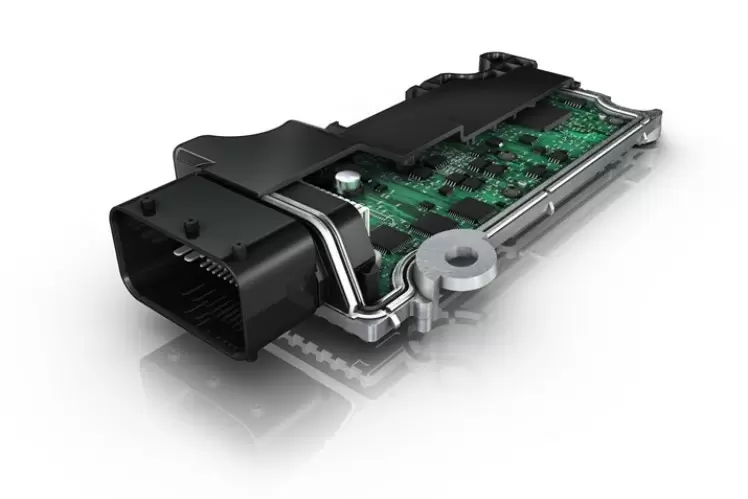
\includegraphics[width=100mm, keepaspectratio]{figures/ecu.png}
	\caption{Referencia kép egy elektronikus vezérlőegységről\cite{ecu}}
	\label{fig:ecu}
\end{figure}

Az elektonikus vezérlőegységekből egy prémium személyautóban akár 100-150 db is létezhet, ezek különböző feladatokat láthatnak el kezdve az ülésmagasság állításától a motor részeinek működtetéséig. Ezek a vezérlőegységek kommunikációs buszokon keresztül kommunikálnak egymással, ezek a buszok lehetnek logikailag vagy akár fizikailag szegmentáltak. Egy ilyen vezérlőegység látható a \ref{fig:ecu} ábrán, a kommunikációs sinek pedig megtekinthetőek egy modern Bentley keresztmetszeti képén a \ref{fig:bentley} ábrán.\\

\begin{figure}[!ht]
	\centering
	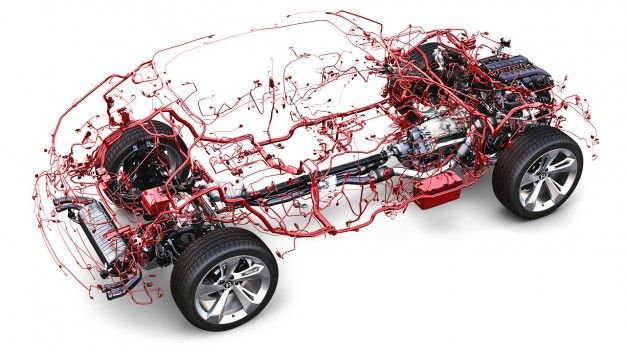
\includegraphics[width=100mm, keepaspectratio]{figures/bentley.jpg}
	\caption{Egy Bentley keresztmetszeti ábrázolásán látható kommunikációs sínek\cite{bentley}}
	\label{fig:bentley}
\end{figure}

Egyes vezérlőegységek képesek lehetnek vezetéknélküli kommunikációra is, fedélzeti számítógép esetén ez lehet WiFi, GPS, Bluetooth, NFC stb., ami nagyban megnövelte a kiberbiztonsági kockázatok mértékét a modern járművekben. 

Ami szintén fontos az még az over-the-air szoftverfrissítés, hiszen ma már nem arra rendezkedik be az autóipar, hogy az eszközein a szoftverfrissítést a szervizből kelljen elvégezni, hanem azt akár távolról, otthonról a garázsból.

Ezek a feltételek jelentik a megnövekedett fontosságát a járművek kiberbiztonságának, azonban érdemes még kiemelni azokat a támadómodelleket amelyek jellemzőek lehetnek az autóiparban, ezzel is felkészülve a lehetséges károkra amelyektől védenénk a rendszert.\\

A bűnözői attitűd lehet egyrészről jellemző, az autólopások már az elektronikus eszközök integrációját megelőzik, azonban azoknak a jelenléte nem minden esetben jelent magasabb fokú biztonságot. Az új elektronikus rendszerek például lehetővé tették azt is, hogy a támadó a fényszóró leszerelésével belépési pontra tegyen szert a járműben, majd azon keresztül oldja fel a zárakat és indítsa el a járművét. Erről bővebben lehet olvasni a Gareth Halfacree cikkében \cite{toyota}.

Szintén érdekes és már régóta az autóipar része a tuningolás, ami a vezérlőegységek mennyisége és azoknak a belső paraméterei miatt ez még nagyobb kontrollt adhat egy jogosulatlan felhasználónak. Állíthat egyrészről akár kormányzási érzet paramétereket, de módosíthat kibocsátási vagy motor működést limitáló értékeket is.

A fizetős extráknak a jailbreak-elése már játék konzolok és telefonok esetén ismert, azonban mióta egyes autógyártók előfizetéses extrává tettek olyan extrákat mint a hátsó ülésfűtés és hasonlók, azóta ez itt is egy természetesen illegális, kártékony tevékenység ami egy támadó célja lehet az ECU ellen. Erre egy példa lehet Arthur Parkhouse cikke \cite{tesla}.

Szintén fontos kiemelni a vírusok (malware, ransomware) telepítését is elektronikus vezérlőegységekre, hiszen a távoli szoftverfrissítés támogatása lehetővé teszi az ezen támadások végrehajtását is.

Végül amit fontos észben tartani, hogy az ezeken tárolt adatokat is fontos védeni, hiszen egy fedélzeti számítógép potenciálisan tárolhat személyes adatokat (personal identifiable information, PII) vagy akár felhasználóneveket, jelszavakat is navigációs és más elérhető alkalmazásokhoz. De maga a tárolt szoftver se kerülhet ki nyilvánosan hiszen az elősegítené a támadóknál a sérülékenységek keresését, azokra automatizált megoldások fejlesztését.


\section{Autóipari kiberbiztonsági szabályozások és szabványok}

Az autóipari kiberbiztonság területe ellentétben az üzembiztonsággal vagy a bővebb IT biztonsággal még csak pár éves múltra tekint vissza, emiatt az itt alkalmazandó szabályozások és szabványok még csak az első változatukban kerültek kiadásra. 

\subsection{UN ECE R155}
Az első specifikusan autóipari szabályozás az Egyesült Nemzetek által kiadott 155-ös számú szabályozás a kiberbiztonságról és a kiberbiztonság kezelő rendszerekről és járművek engedélyeztetésének kapcsolatáról (UN ECE R155\cite{R155}). Ennek a szabályozásnak kell megfelelnie a járműgyártóknak és beszállítóiknak az összes 2024 után megjelenő járműmodell engedélyeztetéséhez.

Ez a szabályozás már tartalmazza az igényt a kockázat-alapú kiberbiztonsági kezelés szükségességére. Ami annyit tesz, hogy a biztonsági szolgáltatásokat az alapján kell meghatározni, hogy egy kiberbiztonsági fenyegetés esetleges bekövetkezése mekkora hatással lenne a védendő autóipari termékre.

Szintén már megtalálhatjuk az autóipari termékek életciklusának különválasztását fejlesztési, gyártási és gyártás utáni fázisokra, ami mutatja azt, hogy a kiberbiztonsági szempontból fontos figyelembe, venni, hogy az életciklus különböző szakaszain más-más fenyegetésekre lehet számítani, és ennek megfelelően más követelmények is lesznek érvényesek a termékre.

A dokumentum a továbbiakban követelményeket határoz meg, hogy milyen folyamatokon kell keresztülmennie egy autóipari terméknek, ahhoz, hogy az a közúti használatra engedélyt kapjon. 

\subsection{ISO/SAE 21434}

A másik, már technikaibb szintű, szintén 2021-es megjelenésű, irányadó szabvány az autóipari kiberbiztonsági mérnökségről szóló ISO/SAE 21434 "Road vehicles - Cybersecurity engineering"\cite{ISO21434}. Ezt a szabványt közösen fejlesztette és adta ki 2021 augusztusában az International Standards Organization (ISO) és a Society of Automotive Engineers (SAE).

Ez a szabvány kezdett el követelményeket megfogalmazni az autóipari rendszerek (E/E) kiberbiztonsági kockázatkezelésének menetére, valamint a biztonság fejlesztésére és kezelésére. A felépítése emlékezetheti az olvasóját a már jóval ismertebb ISO 26262 "Road vehicles - Functional safety" szabványra, amely ugyanazon termékek üzembiztonságának a kezelésére és elemzésére fókuszál.

A szabvány először a tervezési, fejlesztési, gyártási, üzemeltetési, karbantartási és kivezetési fázisokra fogalmaz meg követelményeket, valamint tartalmaz egy fenyegetés elemző és kockázat értékelő eljárást amelynek a Threat Analysis and Risk Assessment (TARA) nevet adták.

Továbbá tartalmaz más követelményeket a kiberbiztonsági elvárások kezelésére különböző menedzsment és organizációs szintekre, azonban ezek ismerete nem tartozik a témám látókörébe.

Dolgozatom kifejezetten a tervezési fázishoz tartozó kockázatelemzés végrehajtására vonatkozó követelményeket veszi alapul. A későbbi bemutatásuk során felfedezhető lesz, hogy a kockázatelemzés iteratív használatának szükségessége az életciklus különböző fázisaiban, azonban a termék üzemeltetési környezetére vonatkozó védelmet ebben a tervezési fázisban határozzuk meg. Ezzel elkerülve a magasabb költségű utólagos fejlesztéseket.

\subsubsection{Követelmények a tervezési fázisra}
A tervezési fázis egy autóipari termék életciklusában a kiindulópont. Az ebben a fázisban végzett kiberbiztonsági tevékenységek célja, hogy (i) definiálásra kerüljön az elemzendő termék, a környezete és interakciói, (ii) meghatározzák a kiberbiztonsági célokat és állításokat valamint, hogy (iii) elkészüljön a kiberbiztonsági terv.

A \textbf{termék definíciója} tartalmazza a termék határait, feladatait, valamint az előzetes architektúrát. Célunk itt az, hogy összegyűjtsük az elemzéshez szükséges információkat.

A \textbf{kiberbiztonsági célok és állítások} meghatározásához szükséges a TARA elvégzése, aminek az eredményeképp születnek meg, az egyes kockázatok kezelésére vonatkozó döntések, amelyek alapján eldönthetjük, hogy a kockázathoz egy célt vagy állítást kell megfogalmaznunk. A cél fogja meghatározni a magas-szintű követelményt amit a termék fejlesztése során figyelembe kell venni, míg az állítás azt határozza meg, hogy az adott kockázat mitigálása valamilyen okból már teljesült vagy a teljesülése szükségtelen.

Ezután készülhet el a \textbf{kiberbiztonsági terv}, amelyben az egyes mitigációkat határozzuk meg a célok elérésére, a célokat tovább finomítjuk követelményekké, majd azokat allokálhatjuk a termékre vagy egyes komponensekre.

\subsubsection{Követelmények a fenyegetéselemzésre és kockázatértékelésre}
A TARA bemenete a termék definíció, és ez alapján lehet elvégezni a hét lépésből álló kockázatelemzési eljárást aminek a kimenete az egyes fenyegetések kockázati értékkel, valamint az azok kezeléséről szóló döntés.

Az első lépése a kockázatelemzésnek az \textbf{érték azonosítás}. Ennek a lépésnek két célja van. Az egyik, hogy a lehetséges \textit{károkozásokat} azonosítsuk és azok segítségével az egyes \textit{értékeket} is meghatározzuk, a másik pedig, hogy az értékekhez \textit{kiberbiztonsági tulajdonságokat} rendeljünk. 
A károkozások tartalmazhatják a kár körülírását, a releváns értékeket és a kapcsolatot a járműfunkcionalitás és a kedvezőtlen következmény között.
Az értékek azonosítására használhatjuk továbbá a termékleírást, a \textit{fenyegetések} definiálását vagy már létező katalógusokat.

A kockázatelemzés második lépése a \textbf{hatásértékelés}. Itt a célunk az egyes lehetséges károkozásokat és azok következményeit valamilyen keretrendszer mentén értékelni. Egy lehetőség, amit több szabvány is említ, az az SFOP alapú értékelés. Az SFOP négy dimenziót határoz meg amiben el kell végezni az értékelést. Ezek az üzembiztonsági hatás (safety), gazdasági hatás (financial), üzemeltetési hatás (operational), valamint az adatvédelmi hatás (privacy).

A kockázatelemzés harmadik lépése a \textbf{fenyegetések azonosítása}, amelyekhez hozzá kell rendelni a támadott \textit{értéket}, annak a kompromittált \textit{kiberbiztonsági tulajdonságát}, valamint a kompromittálás okát. A szabvány szerint ezek azonosítására lehet egyrészről csoportos, brainstorming alapú vagy szisztematikus, keretrendszerek által meghatározott módszereket is alkalmazni. Az utóbbi esetben javasolt valamilyen ismert fenyegetésmodellezési megközelítést használata. Néhány felsorolt példa ezekre az EVITA, TVRA, PASTA és a STRIDE.

A negyedik lépés a \textbf{támadási útvonal elemzés}. Az elemzés során a szabvány szerint top-down vagy bottom-up megközelítést is használhatunk. Előbbi esetben támadási fákat, támadási gráfokat, utóbbi esetben már ismert sérülékenységekre alapulót.

Az ötödik lépés a \textbf{támadás megvalósíthatóságának vizsgálata}, ahol több már létező keretrendszert alkalmazhatunk az egyes támadási útvonalak kiértékelésére. 

A hatodik lépés a \textbf{kockázatiérték meghatározás}. Itt egy egytől ötig terjedő skálán értékeljük a fenyegetési szcenáriókat a hatásértékek és a megvalósíthatósági értékek alapján.

A hetedik és egyben utolsó lépés pedig a \textbf{kockázatkezelési döntés}, amikor az egyes kockázatok kezeléséről hozhatunk döntést. A kockázatokat elkerülhetjük, csökkenthetjük, megoszthatjuk, valamint megőrizhetjük.

Jól látható, hogy ezek a követelmények elég általánosak, sok döntési jogosultságot helyez a folyamatot bevezető személyekre, emellett viszont magas szinten jól körülírt követhető lépéseket határoz meg amelyek megfelelnek más szabályozások feltételeinek és képes eljuttatni a mérnököt a konkrét megvalósítandó intézkedések meghatározásához. 

\section{Fenyegetésmodellezési keretrendszerek és módszerek}

A fenyegetésmodellezés egy olyan folyamat, aminek segítségével azonosítani tudjuk a lehetséges fenyegetéseket, valamint segítenek azok értékelésében.

Ez a folyamat már viszonylag régóta elterjedt a kiberbiztonsági szakmában és támogató jellegű kapcsolatban áll a kockázatelemzésekkel. Amíg a fenyegetésmodellezés célja a fenyegetések meghatározása, a kockázatelemzés az ami segít nekünk a feltárt fenyegetések kezelésének priorizálásában vagy esetenként az egyes fenyegetések elhagyásában.

Tágabb értelemben akár a kockázatelemzést is vehetjük a fenyegetésmodellezés részének, azonban az ISO/SAE 21434 szabványban leírt folyamat is különválasztja azokat és a fenyegetésmodellezést kifejezetten a fenyegetések meghatározására javasolja.

\subsection{CIA és AAA}

Bár még nem is egy teljes fenyegetésmodellezési keretrendszer a CIA háromszög vagy CIA triád, mégis a legtöbb kiberbiztonsági elemzés az ezen betűszó által kifejezett modellt alkalmazza.

Már korábban beszéltünk kiberbiztonsági tulajdonságokról, itt a CIA által definiáltak használjuk, ezek a bizalmasság (confidentiality), sértetlenség (integrity) és elérhetőség (availability). 

Szintén előfordul ennek a modellnek a bővítése egyéb tulajdonságokkal, ilyenek a szoftverbiztonság esetén használt AAA modell elemei amelyek az egyediség (authenticity), engedélyezhetőség (authorizability), valamint az elszámoltathatóság (accountability).

Adott értéknek a tulajdonságait meghatározhatjuk az alábbi kérdések megválaszolásával:
\begin{itemize}
    \item \textbf{Bizalmasság}: Harmadik fél szerezhet-e tudomást az értékről, annak tartalmáról?
    \item \textbf{Sértetlenség}: Az érték módosulása vezethet-e nem várt következményekhez?
    \item \textbf{Elérhetőség}: Az érték hiánya vezethet-e nem várt következményekhez?
    \item \textbf{Egyediség}: Kell-e az érték eredetét biztosítani felhasználása előtt?
    \item \textbf{Engedélyezhetőség}: Szükséges-e az adott értékhez való hozzáférés korlátozása?
    \item \textbf{Elszámoltathatóság}: Szükséges-e az adott értékhez való hozzáférések, módosulások visszakövethetősége?
\end{itemize}

A továbbiakban ezeket a modelleket fogom alkalmazni a kiberbiztonsági tulajdonságokként, azonban ezek módosíthatók, elhagyhatóak, cserélhetőek és bővíthetőek felhasználási környezetüktől függően. Az én esetemben a CIA elegendő lesz, hiszen autóipari beágyazott rendszerekben a szoftver szinten azon tulajdonságok relevánsabbak. Az üzenet egyediségének hamisítása már az eredeti üzenet egyfajta sérülését vonja magával, ez a sértetlenség tulajdonság által már kezelve van. Az engedélyezhetőség pedig már bonyolultabb operációs rendszerek használatánál kerül elő, ami külön felhasználókat és hozzáféréseket tud definiálni. Ez bizonyos formában az autóiparban is fellelhető, de nem abban a komplexitásban mint Linux vagy Windows alapú rendszereknél. Az elszámoltathatóság szintén problémás mivel ennek a biztosítása, a beágyazott rendszerek limitált hardvererőforrásai miatt nem tud azzal a granularitással létezni, ahogy a hozzáférések számon lennének tartva IT rendszereknél.

\subsection{STRIDE}
A STRIDE egy modell, amely számítógépes kiberbiztonsági fenyegetések azonosítására lett kifejlesztve a Microsoft által 1999-ben. A nevét a hat fenyegetéstípusról kapta, ezek és a jelentésük:

\begin{itemize}
    \item \textbf{Spoofing:} Megszemélyesítés, amikor a rendszer hamisan érzékeli az információ küldőjének a kilétét
    \item \textbf{Tampering:} Valamilyen információ megváltoztatása
    \item \textbf{Repudiation:} Annak az állítása, hogy valamit nem te csináltál vagy nem is történt meg
    \item \textbf{Information disclosure:} Egy támadó képes hozzáférni olyan információhoz amire nincs jogosultsága
    \item \textbf{Denial of Service:} Erőforrások túlterhelése miatt szolgáltatás elérhetetlenné tétele
    \item \textbf{Elevation of privilige:} Egy támadó képes olyan művelet elvégzésére, amire nincs felhatalmazva
\end{itemize}

Ez első ránézésre egy jó lehetséges kategorizálást ad meg nekünk fenyegetésekhez, valamint kibővíthető ezek kapcsolata az azonosított értékekhez és kiberbiztonsági tulajdonságaikhoz. Tehát az egyes fenyegetés típusok egy bizonyos tulajdonság sérülését célozzák.

\begin{table}[h]
    \centering
    \begin{tabular}{rl}
        Spoofing & Egyediség (authenticity) \\
        Tampering & Sértetlenség (integrity) \\
        Repudiation & Letagadhatatlanság (non-repudiability) \\
        Information disclosure & Bizalmasság (confidentiality) \\
        Denial of Service & Elérhetőség (availability) \\
        Elevation of privilige & Engedélyezhetőség (authorizatiability) \\
    \end{tabular}
    \caption{Fenyegetések kapcsolata kiberbiztonsági tulajdonságokkal}
    \label{tab:my_label}
\end{table}

Ebből jól látható, hogy az egyes értékekhez a tulajdonságaik alapján már azonosíthatjuk az azok kompromittálását célzó lehetséges fenyegetéseket.

Ezekből én mivel csak a CIA tulajdonságait használom, az én esetemben a Tampering, Disclosure és Denial fenyegetések lesznek a tulajdonságokból származtatva.

\section{Autóipari rendszerek általános tervezése és modellezése}

A diplomamunkám sajátossága abból adódik, hogy amíg az általános IT rendszereknek vagy azok egyes elemeinek az architektúrális tervezése kevésbé jellemző, addig a kiber-fizikai rendszereknél, azon belül is a járműveknél, a rendszer komplexitása és az üzembiztonság kritikussága miatt, nagy hagyománya van ezeknek az átfogó dokumentálására már a tervezés kezdeti szakaszában.

\subsection{V-modell}

A V-modell egy szoftverfejlesztési folyamat amelyet az ASPICE szabvány adaptál az autóiparban. Lényegében arról szól, hogy a fejlesztés V alakban történik, ahol bal oldalt fentről lefele történik a tervezés és a fejlesztés, a jobb oldalon pedig minden lépéshez tartozik egy verifikációs vagy validációs lépés.

Nemrégiben kapott az ASPICE\cite{ASPICE} szabvány egy kiegészítést a kiberbiztonsági mérnöki folyamatokhoz amelyeket részben az ISO 21434 is definiált. Ezekről egy összefoglaló a \ref{fig:ASPICE} ábrán látható.

\begin{figure}[!ht]
\centering
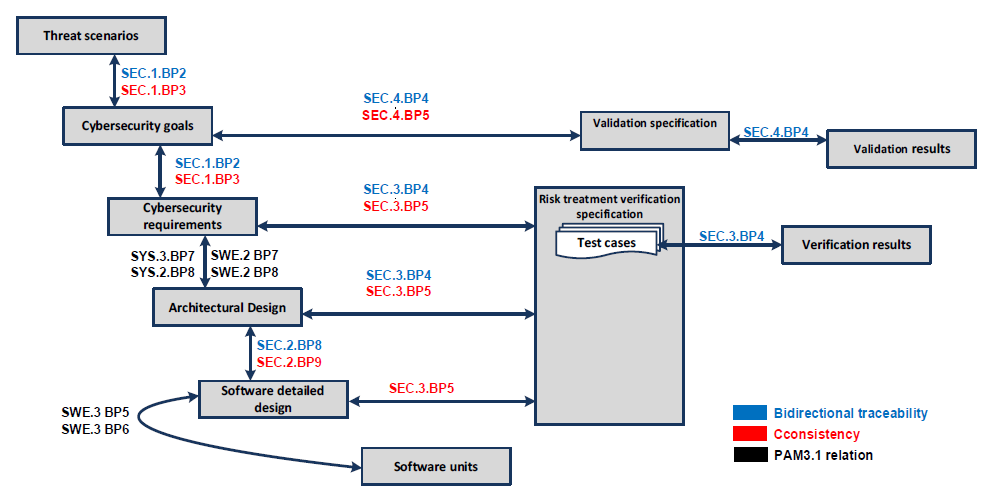
\includegraphics[width=150mm, keepaspectratio]{figures/02_ASPICE.png}
\caption{Az ASPICE javaslata kiberbiztonsági folyamatokra\cite{ASPICE}}
\label{fig:ASPICE}
\end{figure}

Szintén érdemes itt megjegyezni, hogy az általam javasolt metodológia egyfajta visszacsatolást (feedback) tenne lehetővé az \textit{Architectural design} és a \textit{Threat scenarios} lépések közt. De erről később bővebben lesz szó.

\subsection{UML és SysML}

A komplex E/E architektúrák esetén, mint amilyenek az autóipari beágyazott rendszerek, jellemző valamilyen formában a rendszermodellek jelenléte és karbantartása a termék életciklusa alatt. Erre elsősorban a SysML (System Modeling Language) van használva, ami egy bővítése az UML-nek (Unified Modeling Language).\\

% UML
Az UML egy általános felhasználású grafikus modellezési nyelv, amelynek célja a rendszerek specifikálása, a felépítésük leírása, vizualizálása és dokumentálása a fejlesztésben érdekelt minden résztvevő számára.

Az UML több diagram típust különböztet meg, azokat elsősorban két kategóriába sorolhatjuk, az egyik a strukturális a másik pedig a viselkedési diagramok. A strukturális diagramok közé tartozik a csomag, a komponens, az objektum, az osztály, a kompozit, a profil és a telepítési diagramok. A viselkedési diagramok közé pedig az aktivitás, az állapotgép, a használati eset, a kommunikációs, a szekvencia, és az időzítési diagramok.

Az UML szintén támogatja a modellezési nyelvnek egy adott doménre való szabását. Ezt profilok definiálásával lehet megtenni. A profilokra érdemes úgy gondolni, mint az UML egyfajta bővítményei, amelyeket bizonyos modell elemekre tudunk rászabni.\\

% SysML - subset

A SysML az UML nyelvi elemei egy részhalmazának további nyelvi elemekkel bővített verziója. Ezeket a bővítéseket egy SysML profillal implementálják és elsősorban ezt a nyelvet használják a komplex hardver-szoftver rendszerek modellezésére.\\

% Használat

Az én megoldásom az alap UML bővítéseképp tartalmaz egy kiberbiztonsági profilt, mivel a SysML bővítményei nem voltak elegendők az autóipari rendszerek kiberbiztonsági elemzésére, tervezésére. A termék leírására, valamint a kockázatelemzés érték és károkozás definíciós szakaszára egy használati eset (use case) és egy komponens (component) diagramot használok.

\section{Felhasznált eszközök}

\subsection{Papyrus}

A Papyrus egy nyílt forráskódú UML 2 modellező eszköz. Ezt az eszközt fogom használni az értékek definiálására egy komponens diagramon valamint a károkozásokat egy használati eset diagramon keresztül.

Ebben az eszközben definiálok továbbá egy kiberbiztonsági profilt, ami bővítményeket tartalmaz a komponensekhez és a használati esetekhez.

\subsection{Acceleo}

Az Acceleo egy nyílt forráskódú Model-2-Text (M2T) eszköz, amellyel a Papyrus-ban definiált modellekből fogom generálni a kiberbiztonsági elemző eszköz kiinduló modelljét. Más szóval ezzel az eszközzel származtatom a rendszermodellből a kiberbiztonsági modellt.

Azért eset a választásom erre az alkalmazásra az Xtend helyett, mivel az integrációja a Papyrus eszközzel sokkal jobban támogatott, illetve mivel nincs szükség nagy komplexitású kódgenerálásra.

\subsection{Eclipse Modelling Framework}

Az Eclipse Modelling Framework, vagy röviden EMF egy modellezési keretrendszer ami arra ad támogatást, hogy könnyen lehessen modellező eszközöket, majd ahhoz kódgenerátor alkalmazásokat fejleszteni.

Az EMF támogatja modellek definiálását, majd azokból automatikusan Java kódot származtat, ezzel elősegítve a modell könnyebb transzformációját, módosítását és abból való származtatást.

Az EMF szintén ad egy automatikusan generált kezelőfelületet a definiált modell szerkesztésére, tartalommal feltöltésére.

Ezt a keretrendszert használtam a kiberbiztonsági elemző eszköz metamodelljének definiálására, továbbá az eszköz kezelő felülete is a generált szerkesztő felületre épül.

\subsection{Xtend}

Az Xtend egy Java alapú programozási nyelv amelyet elsősorban kódgenerálási célokra lehet használni.

Ezt a nyelvet használtam arra, hogy elkészítsem először a modellből való generálását a szabványos dokumentumoknak, majd a támadási fák inicializálását is.

\subsection{Sirius}

A Sirius egy nyílt forráskódú szoftverprojekt amelynek a célja, hogy könnyen lehessen grafikus felületeket létrehozni domén specifikus modellekhez Eclipse-ben.

Ez a keretrendszer volt használva a támadási fák megjelenítéséhez és azok szerkesztésére használt grafikus felület létrehozására.
\chapter{Kapcsolódó tanulmányok}
Ennek a fejezetnek célja, hogy összefoglaljam a diplomamunkámhoz előzetesen elvégzett kutatómunka során megismert tanulmányok eredményeit, problémáit, valamint a lehetséges alkalmazásukat az a feladatom elkészítése során.

A kutatómunkámat három témában végeztem, az első a fenyegetésmodellezés (threat modeling) területe volt. Ezen kutatásokon keresztül ismertem meg a fenyegetések felmérése során felmerülő problémákat, megoldásuknak módjait, azok lehetséges megjelenítését és modellezését.

A második téma az autóipari biztonsági elemzések területén készült munkák kutatása volt, hogy meg tudjam ismerni milyen komponenseket és azoknak mely attribútumai lesznek használhatóak egy elemzés során. Szintén tartalmaztak a kutatások olyan metodológiákat és best practice-eket amelyeket a saját analízis metodológiám során is fel tudtam használni.

A harmadik, utolsó és egyben a legspecifikusabb téma, a már meglévő kutatások amelyek támadási fák (attack trees), illetve támadási gráfok (attack graphs) generálásáról szóltak, ezek az üzembiztonság területén elterjedt hibafa (fault tree) analízis eszközének adaptációi a kiberbiztonsági terület támogatására.

\section{Fenyegetésmodellezés}

Az első témába illő kutatás a Karahasanovic et al.\cite{Karahasanovic} kutatása volt "Adapting Threat Modelling Methods for the Automotive Industry" címmel. Ez két fenyegetésmodellezési keretrendszert mutat be, egyik az Intel-hez köthető TARA (Threat Agent Risk Assessment), ami nem összekeverendő az azonos rövidítéssel fémjelzett Threat Analysis and Risk Assessment metodológiával amit az ISO 21434 definiál, a másik pedig, a sokkal ismertebb Microsoft által fejlesztett STRIDE. 

Az előbbi a grafikus modellezési technikák helyett egy könyvtárakon alapuló fenyegetés elemzést mutat be, ahol három könyvtárat használnak, egyik a lehetséges támadó ágenseket, másik az általuk véghezvihető támadásokat a harmadik pedig, a jellemző támadási felületeket gyűjti. 

A kutatás ezen könyvtárakból határoz meg egy részhalmazt ami az autóipari rendszerek ellen alkalmazható. A második technika már a támadó-centrikusság helyett inkább szoftver-centrikus irányt követi, ami egy fehér doboz vizsgálatot tesz lehetővé a rendszeren. Ez, a későbbiekben még előforduló Data Flow Diagramok használatára mutat be egy példát amelyben a szoftver komponensek közti kommunikációt modellezi és tud egy támadási útvonalat végigkövetni. 

Az előbbi technika gyengesége az, hogy csak magas szinten definiálja a fenyegetéseket ami nem elégséges a védelmi mechanizmusok meghatározására. Utóbbi ezzel szemben alkalmas arra, viszont nem lehet vele rendszer szintű védelmet modellezni, valamint tervezési fázisban is nehezen alkalmazható.\\

Ma et al.\cite{Ma} kutatása "Threat Modeling for Automotive Security Analysis" címmel, a fenyegetésmodellezést egy sokkal gyakorlatibb módon közelíti meg, nem feltétlenül a technikai részekre koncentrál, hanem a termékfejlesztési életciklust és a már meglévő üzembiztonsági analíziseket is figyelembe veszi. 

Helyesen jelzi a szükségét az analízis szintekre bontásának, hasonlóan az üzembiztonsághoz, azonosítja az igényét egy funkcionális kiberbiztonsági tervnek valamint egy technikai kiberbiztonsági tervnek, kiegészítve egy termékspecifikációval. Ezeknek a jelenlétét pedig lebontja az elsőt a tervezési fázisban, magas szintű követelmények azonosításához, a másodikat termékfejlesztési szakaszhoz, bemenetként a rendszermodellt használva, a specifikációt pedig gyártási fázisban való használattal. 

A kutatás tartalmaz még egy esettanulmányt amely, egy jármű utasterének a biztonsági analízisén vezet végig, a Microsoft Threat Modelling Tool használatával, ami a STRIDE keretrendszerre épít, data flow diagramokat használ és modell alapon generál lehetséges fenyegetéseket. 

Konklúzióként emeli ki az igényt, hogy a biztonsági analízis modellezési paradigmáit, valahogyan integrálni szeretnék a rendszermodellezés paradigmáival, ezzel biztosítva, hogy az analízis a változások során napra kész maradjon. A termékfejlesztési fázisok és kiberbiztonsági elemzéseket a \ref{fig:MA} ábrán részletezik.\\

\begin{figure}[!ht]
\centering
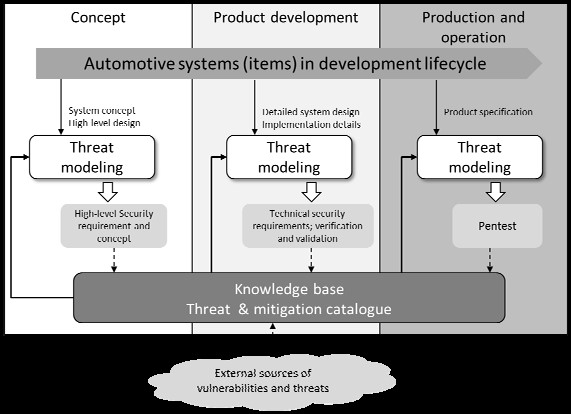
\includegraphics[width=125mm, keepaspectratio]{figures/03_MA.png}
\caption{Fenyegetésmodellezés a termékfejlesztési életciklusokban\cite{Ma}}
\label{fig:MA}
\end{figure}

Ehhez a területhez tartozik még Vivek et al.\cite{Vivek} kutatása ami egy esettanulmány volt, egy tetszőleges autóipari komponensre, kiértékeléshez egy módosított STRIDE modellt használt, valamint az ISO 21434-ben definiált kockázatelemzés kezdeti lépéseit amelyek a lehetséges fenyegetések feltárására vannak alkalmazva.

\section{Kiberbiztonság és üzembiztonság kapcsolata}

Ezzel a témával kapcsolatban Dantas et al. \cite{Dantas} kutatása mutatja be, hogy a szabványosított kockázatelemzésre, hogyan lehet már meglévő technikákat alkalmazni valamint, hogy a kockázatelemzés, hogyan illeszkedik be már létező folyamatokba. 

A dokumentum részletesen elemzi a kiberbiztonság fontosságát az autóiparban, valamint a szoftverfrissítés jelenlétét mint fontos eszközt esetleges sérülékenységek javításában. Szintén elemezve van a rendszeres és folyamatos auditálása és kiértékelése ezeknek a folyamatoknak. Ezekhez jelzi a lehetőséget különböző domén-specifikus nyelvek használatának lehetőségét és automatizálás integrálását, illetve modellellenőrző rendszerek bevezetését. 

Van még szó az üzembiztonság területén alkalmazott FTA (Fault Tree Analysis) és FMEA (Failure Modes and Effects Analysis) technikájának felhasználásáról a támadási útvonalak elemzésében, illetve idéz több más tanulmányt és keretrendszert amelyek szintén ezen alkalmazásokat ösztönzik.\\

Bohner et al.\cite{Bohner} kutatása az üzembiztonsági architektúrát terjesztené ki a kiberbiztonsági kockázatok kezelésére. Helyesen hívja fel a figyelmet arra, hogy a kiberbiztonsági elemzések alapjául használt CIA triádból kettő, az integritás (integrity) valamint a rendelkezésre állás (availability) az üzembiztonság területén már véletlenszerű hibák esetére alkalmazva vannak. 

Említésre kerülnek itt a memória particionálás mint ami a két területen csökkentik a kockázatot, az üzenetek védelmét módosítás ellen, valamint összességében a kiberbiztonság mint részhalmaza az üzembiztonságnak ahol a véletlenszerűen előforduló hibák helyett a szándékosan okozott hibákat kell figyelembe vennünk. A kockázat csökkentő intézkedések alkalmazása pedig szignifikánsan tudja mind a két fajta biztonság hatékony szolgáltatását.\\

Chulp et al.\cite{Chulp} kutatása egy ThreatGet nevezetű kiberbiztonsági kockázatelemző eszköz működési elvét mutatja be amely a bécsi egyetemen készült. Ez az eszköz gyakorlatiasan írja le a tervezési fázisban elvégzendő kockázatelemzés menetét, ebben már az ASPICE-szal ellentétben láthatunk feedback alkalmazását a folyamat lépései közt és egy külön modellt is használ kockázatelemzésre amelyet össze hasonlítana a meglévő rendszermodellel, ahogy az a \ref{fig:CHULP} ábrán látható.

Chulp et al.\cite{Chulp} kutatásában továbbá hasonlóan az én munkámhoz a STRIDE fenyegetésmodellezési keretrendszert valamint a CIA triád közös használatát végzik el. Szintén érdemes kiemelni a fenyegetésmodellezésre jellemzően használt Data Flow diagram kiegészített formáját amelyet Extended Data Flow diagramnak neveznek, ebben egy részről kompozíciók modellezését teszik lehetővé, másrészről pedig értékek (asset) megjelenítéséről is gondoskodtak. Ez a modell már sokkal alkalmasabb komplex kiber-fizikai rendszerek elemzésére az általános Data Flow diagrammokkal szemben. Ez a diagram a \ref{fig:CHULP_EDD} ábrán látható.

\begin{figure}[!ht]
	\centering
	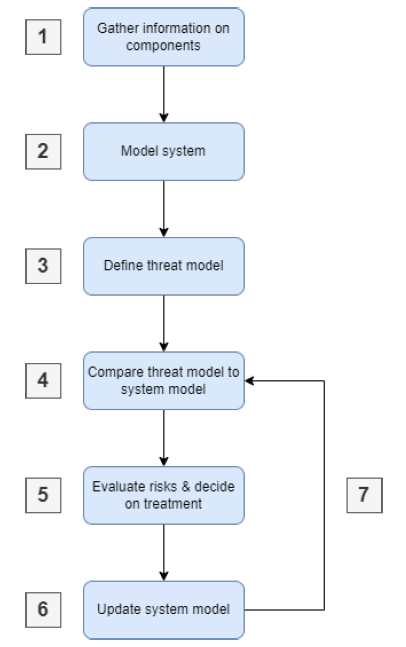
\includegraphics[width=75mm, keepaspectratio]{figures/03_CHULP.png}
	\caption{Fenyegetésmodellezés folyamata a tervezési fázisban\cite{Chulp}}
	\label{fig:CHULP}
\end{figure}

\begin{figure}[!ht]
	\centering
	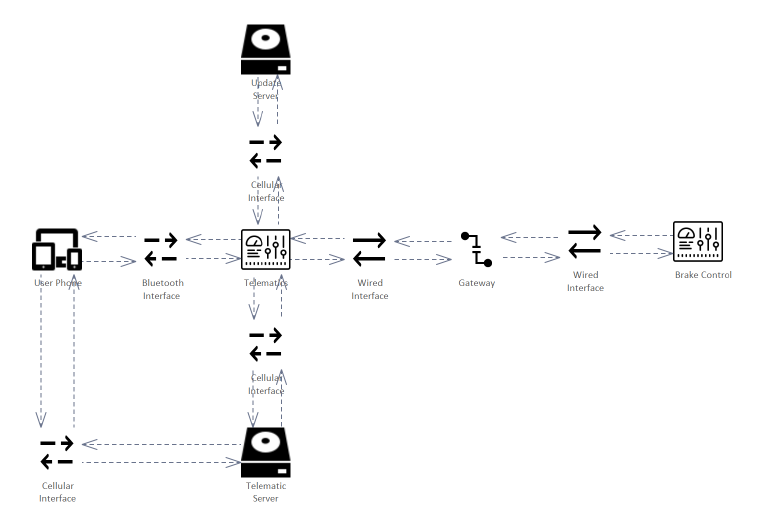
\includegraphics[width=125mm, keepaspectratio]{figures/03_CHULP_EDD.png}
	\caption{Extended Data Flow diagram grafikus megjelenítése\cite{Chulp}}
	\label{fig:CHULP_EDD}
\end{figure}

Ebben a kutatásban hangzik el először az automatizált támadási fa generálásának fogalma, valamint a tanulmány támadási gráfokat is definiál. A kutatás jól használja fel az Extended Data Flow Diagram rendszermodelljét támadási fák és gráfok generálására amelyekből támadási utakat vezet le amelyek alkalmasak lesznek valódi kockázatok meghatározására.

Magukról a támadási fákról alkotott modell pedig a \ref{fig:CHULP_AT} ábra mutatja be. Ezen nehezen látható, hogy az Extended Data Flow diagramból (ami a \ref{fig:CHULP_EDD} ábrán látható) lenne származtatva a modell, valamint a végeredmény egy absztrakt megfogalmazású és nem kifejezetten az egyes komponensekre irányuló támadásokat jelenít meg a támadás lépéseiként. Szintén a dependenciák is kevésbé használják ki a logikai kapuk nyújtotta felépítés lehetőségeit.

\begin{figure}[!ht]
	\centering
	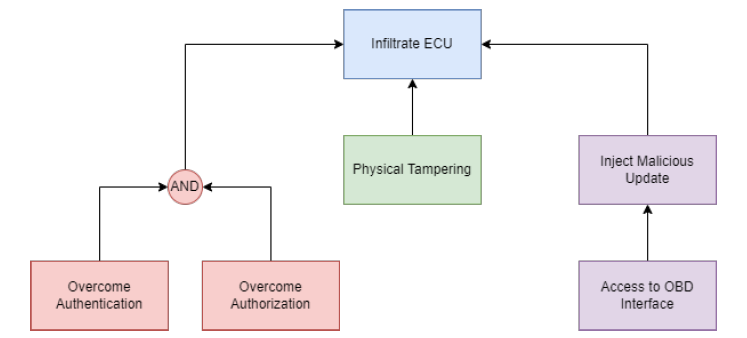
\includegraphics[width=125mm, keepaspectratio]{figures/03_CHULP_AT.png}
	\caption{Támadási fák grafikus megjelenítése\cite{Chulp}}
	\label{fig:CHULP_AT}
\end{figure}

\section{Támadási fa generálás}

Sowka et al.\cite{Sowka} publikációja különböző alkalmazásait értékelte az automatikus támadási fáknak az autóipari kiberbiztonság doménjében. Az írás ad egy általános áttekintést a terület fontosságáról, a szabályozási környezet aktuális helyzetéről majd összehasonlította a különböző elérhető megoldásokat az adott problémára.

A Salfer et al.\cite{Salfer} kutatása által bemutatott módszer egy magas fokú modellezett megoldás alapján való támadási utak előállítását határozza meg. Kifejezetten érdekes, ahogy felépíti a metamodelljét amiben definiál egy rendszer és egy támadó modellt is. A rendszermodell meghatározza az elektronikus vezérlő egységeket, szoftvereket, kommunikációs hálózatokat és értékeket (\textit{asset}), a támadó modell pedig tartalmazza a tudást, motivációt, amelyek aztán a támadások megvalósíthatóságának értékelésében játszanak szerepet. Szintén elemzi ezeknek a támadási utaknak az alkalmazását a rendszer kiberbiztonsági (penetrációs) tesztelésénél és jól ismeri fel, hogy ez egy magasszintű white-box tesztelésben lehetne felhasználható. 

Karray et al.\cite{Karray} kutatása sokban épít az előző bekezdésben említettre, azonban itt nem lehet egy explicit támadómodellről beszélni. A rendszermodell használ bizonyos tulajdonságokat amelyek jelzik a támadó szükséges tudását vagy belépési szükségét, viszont kevesebb feltevést használ a támadások meghatározásánál. A gráf trnaszformáció valamint a rendszermodell még alkalmas lehet a saját munkámhoz.

Végül pedig Bryans et al.\cite{Bryans} kutatását néztem meg amely kombinálja a modell alapú valamint a könyvtár alapú automatizált generálást, azaz a modell és template alapú támadási fa generálást. A Chulp et al.\cite{Chulp} kritikája alapján is ez volt kiemelve mint legérettebb megoldás, valamint ez is az egyik legfiatalabb. A támadó modell helyett előredefiniált támadási mintákat használ fel, amelyek segítségével rekurzívan tud a fa leveleiből kifejteni komplexebb támadásokat egyfajta bottom-up megközelítésben. A rendszermodell szemben a template-ekkel sokkal egyszerűbb, nem különít el ECU funkcionalitást vagy értékeket, emiatt ez a része nem lesz használható a munkám során, viszont ez teszi lehetővé teszteléskor a black-box megközelítést, valamint akár teszt kódok és eszközök integrációjával is lehetne használni deszkriptív template-ek esetén. Célom az, hogy ezt a fajta kombinált megközelítést alkalmazzam erősebben rendszermodellezett megközelítéssel és egyszerűsítettebb template-ekkel.

%\include{content/035_ecu_cybersecurity}
\chapter{A kiberbiztonsági analízis metodológiája}

A diplomamunkám legfontosabb része a metodológia előállítása volt. A metodológia az ami biztosítja azoknak a céloknak az elérését, hogy az analízis (i) teljes körű legyen, (ii) megismételhető legyen és (iii) már létező információkra építsen, azon túl, hogy az eredménye és használata minél átláthatóbb legyen a stakeholderek és az elemző mérnök számára is.

Ez a metodológia kapcsolja össze az autóiparra jellemző rendszermodelleket a fenyegetésmodellekkel. Ennek segítségére és támogatására készült el a kapcsolódó modellező eszköz és ennek az eredménye az egyik legfontosabb előállított értéke a kiberbiztonsági mérnök feladatkörnek.

Az \textit{Áttekintés} fejezet tartalmaz egy magas szintű végigvezetést a bemenetektől a kimenetig és a közte megtett lépésekről.

A \textit{Termékleírás és fenyegetésmodell származtatása} mutatja be a kiindulómodell elkészítésének lépéseit valamint, hogy abból, hogyan állítjuk elő a fenyegetés modellt.

A \textit{Fenyegetésmodellezés} fejezetben láthatóak a további lépések a fenyegetésmodell specifikálására, valamint be mutatja a fenyegetésmodellből előállított támadási fák konstrukcióját és annak szerkesztésének lépéseit.

A \textit{Dokumentumok generálása és manuális analízis} fejezetben pedig találhatóak a szabvány által előírt output előállítása és az elemző eszköz használatát követő folyamatok.

\section{Áttekintés}

A metodológiám fő feladata a \textit{Háttérismeretek} fejezetben található \textit{Követelmények a fenyegetéselemzésre és kockázatértékelésre} részben leírtakat követve kialakítsam azt a lépéssorozatot amelyet az általam fejlesztett eszköz támogatásával végre lehet hajtani és el lehet jutni egy általános autóipari modellből a kockázatelemzés eredményéig.

A lépésekről egy áttekintés a \ref{fig:04_OVERVIEW} ábrán látható. Itt egyrészről a fehér hátterű négyzetekben az ISO 21434 által definiált lépések láthatóak amelyek bővebb leírása a \textit{Háttérismeretek} részben található, lila hátterű négyzetekben pedig az ebben a fejezetben bemutatott lépések láthatóak. Így látható egy egyszerűbb áttekintés a két módszertan közti fedettségről.

\begin{figure}[!ht]
	\centering
	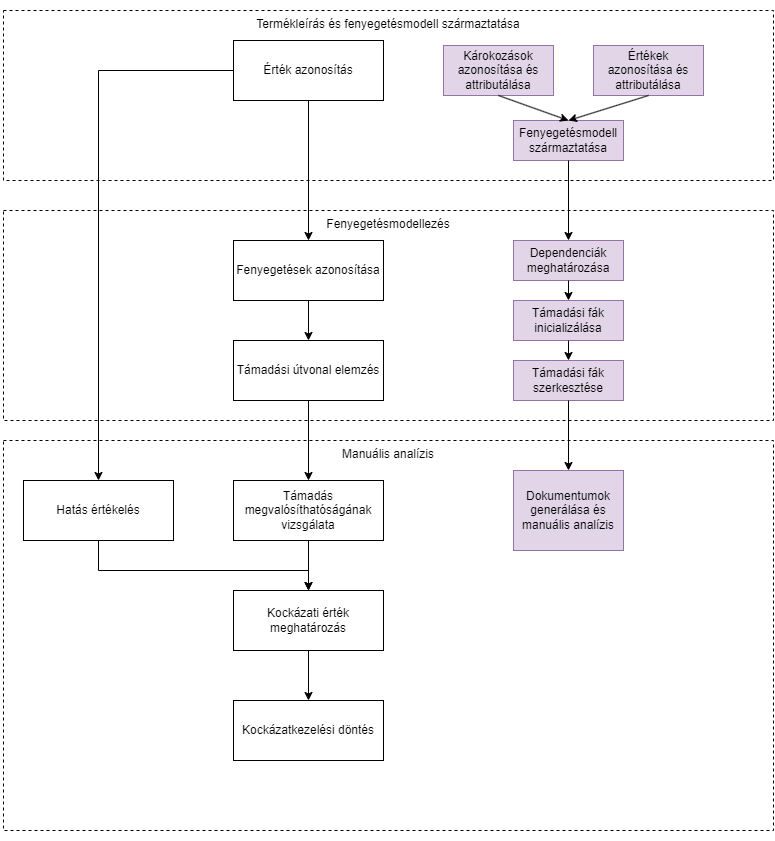
\includegraphics[width=130mm, keepaspectratio]{figures/04_overview.png}
	\caption{Metodológia áttekintése}
	\label{fig:04_OVERVIEW}
\end{figure}

\section{Termékleírás és fenyegetésmodell származtatása}

Ez a fejezet mutatja be az első lépéseit a kockázatelemzési folyamatnak. Itt lesz szükségünk a kiinduláskor rendelkezésünkre álló termékleírást (ami a rendszermodell egy részhalmaza) bővíteni kiberbiztonsági attribútumokkal majd abból származtatni egy olyan új modellt ami a kiberbiztonsági elemzésre alkalmas lesz.

\subsection{Károkozások azonosítása és attributálása}



\subsection{Értékek azonosítása és attributálása}

\subsection{Fenyegetésmodell származtatása}

\section{Fenyegetésmodellezés}

\subsection{Dependenciák meghatározása}

\subsection{Támadási fák inicializálása}

\subsection{Támadási fák szerkesztése}

\section{Dokumentumok generálása és manuális analízis}
\chapter{A kiberbiztonsági analízis megvalósítása}
% Technikai leírása a modellező eszköz architektúrájának
A következő fejezetnek a célja, hogy bemutassa az előző fejezetek által körülírt metodológia végrehajtását segítő fenyegetésmodellező eszközt, valamint a rendszermodellek származtatására készített szkriptet.

Az első alfejezetben látható egy áttekintés majd két fő részre osztva láthatóak a további alfejezetek. A két fő rész egyike a rendszerből kiberbiztonsági modell transzformálást mutatja be és az ezt segítő eszközöket. A másik pedig az EMF alapon implementált modellező eszközt amely a kiberbiztonsági modell alapján képes a manuális analízist támogatni dokumentumok generálásával valamint a támadási fák szerkesztésével.

\section{Áttekintés}

Egy áttekintése az elemző eszköz részeinek megtekinthető a \ref{fig:04_OVERVIEW} ábrán.

\begin{figure}[!ht]
	\centering
	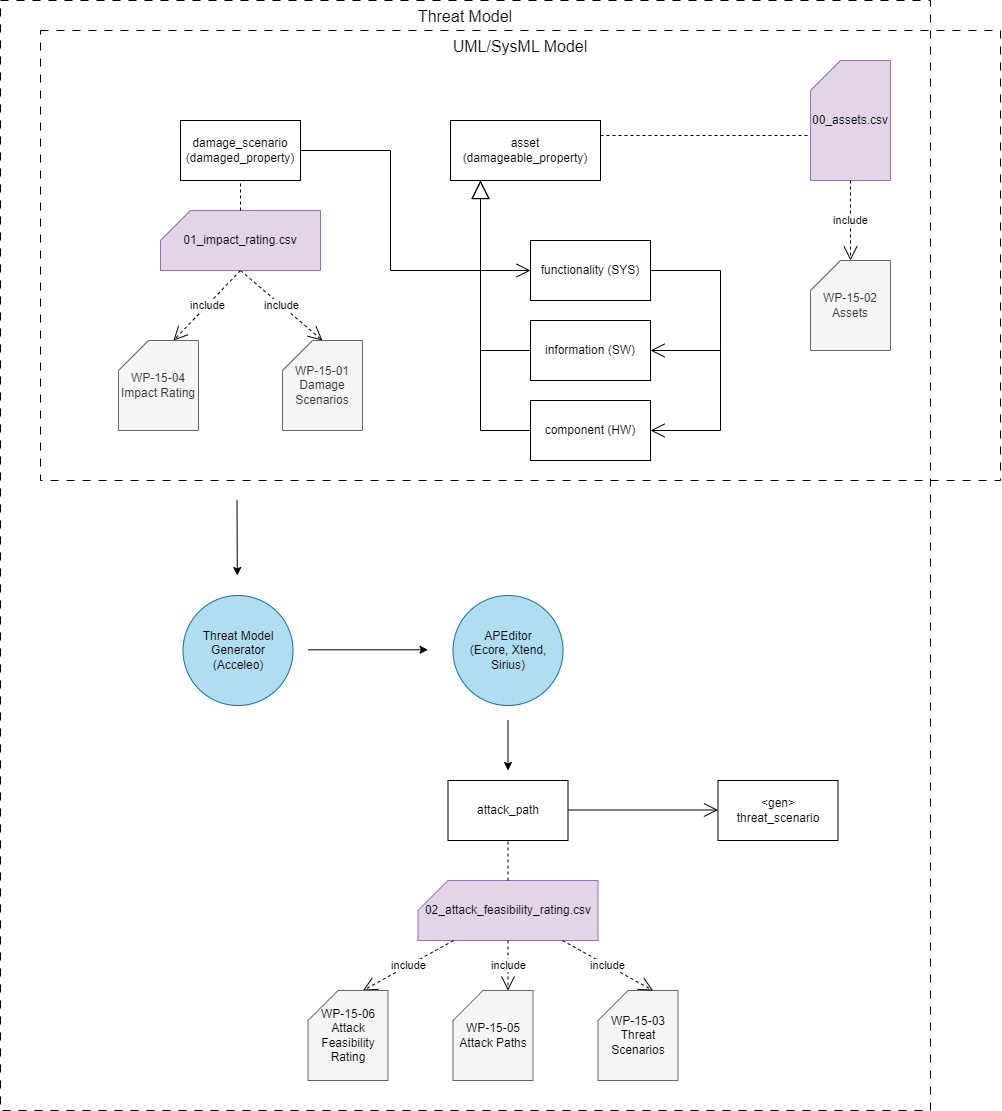
\includegraphics[width=130mm, keepaspectratio]{figures/05_overview.png}
	\caption{Megvalósítás áttekintése}
	\label{fig:05_OVERVIEW}
\end{figure}

Itt először kiemelném a fenyegetésmodell és a rendszermodell közös halmazában lévő tartalmakat. Ez a rendszermodell egy Papyrus projekt formájában készült el. Tartalmazza a \textit{Kihasználási eset diagramot} és a \textit{Termékleírást}. Ezek tartalmazzák az értékeket, funkcionalitást és a lehetséges károkozásokat, amelyekből két dokumentum állítható majd elő, amelyek három ISO 21434 workproduct-ot fednek. 

A következő elem a Threat Model Generator ami egy Acceleo script a Papyrus modellező eszközhöz integrálva és a cybersecurity profil alapján állít elő egy kezdeti modell fájlt amelyet a fenyegetésmodellező eszközzel fogunk tudni megnyitni.

A fenyegetésmodellező eszköz az APEditor (Attack Path Editor) amelyben lehetőségünk van a termékleírás és kihasználási diagram tartalmai közti dependenciák meghatározására, valamint támadási fák és fenyegetések automatikus származtatására.

A támadási fák elkészítése után fogjuk tudni a modellből származtatni a támadás megvalósíthatóság értékelés dokumentumot ami további három ISO 21434 workproduct-ot fed le.

\section{Kiberbiztonsági modell származtatása}

A kiberbiztonsági modell származtatása egy fontos lépése a kockázatelemzési folyamatnak. Előkészíti a fenyegetésmodellünket illetve teremt egyfajta nyomon követhetőséget a rendszermodell és a kiberbiztonsági modell között.

\subsection{Kiberbiztonsági profil}

A profilban négy sztereotípia került meghatározásra. Egyrészről a UseCase UML metaosztályát bővíti a damage\_scenario sztereotípia amellyel a károkozásokat tudjuk jelölni. A károkozásokhoz fel lett véve attribútumként, hogy azt mely kiberbiztonsági tulajdonság sérülése okozta.

A Component UML metaosztályt bőviti a functionality, component illetve az information sztereotípia. Itt a functionality jelenti a rendszerszintű funkcionalitást, ennek nincsenek az UML profilban attribútumai mivel azokat majd a kapcsolódó károkozások alapján fogjuk tudni meghatározni az elemzés későbbi fázisában. A component jelzi a HW komponenseket (pl. csatlakozó, modulok, áramkörök), az information pedig a SW szintű információkat (pl. szoftver, kriptográfiai adatok, üzenetek). Az utóbbi kettő az Asset (\textit{érték}) absztrakt osztályból van származtatva, ebből öröklik a kiberbiztonsági tulajdonságaikat.

\begin{figure}[!ht]
	\centering
	\includegraphics[width=130mm, keepaspectratio]{figures/05_Profile_Diagram.PNG}
	\caption{Kiberbiztonsági profil (UML)}
	\label{fig:05_UML_PROFILE}
\end{figure}

\subsection{Fenyegetésmodell generátor}

A fenyegetésmodell generátor egy Acceleo nyelven írt szkript, amelynek a feladata a Papyrus-ban szerkesztett .uml fájloknak a beolvasása és a tartalmuk alapján egy .apeditor fájlnak a generálása, amelyet a fenyegetésmodellező eszközben lehet tovább szerkeszteni.

A projekt felépítése és a dependenciák a \ref{fig:05_tmgen_arch} ábrán láthatóak.

\begin{figure}[!ht]
	\centering
	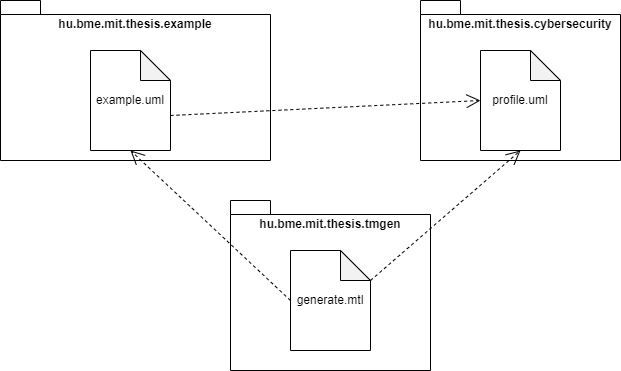
\includegraphics[width=130mm, keepaspectratio]{figures/05_package_tmgen.png}
	\caption{Threat Model Generator dependenciái}
	\label{fig:05_tmgen_arch}
\end{figure}

A \textbf{hu.bme.mit.thesis.example} projekt tartalmazza a kihasználási eset diagramot és a termékleírást, valamint applikálja a \textbf{hu.bme.mit.thesis.cybersecurity} projektben definiált kiberbiztonsági profil sztereotípiáit.

A \textbf{hu.bme.mit.thesis.tmgen} tartalmazza a \textbf{generate.mtl} fájlt ami egy Acceleo nyelven írt Model-To-Text generátor. Ez fogja előállítani a projekt \textit{generated} mappájába az \textbf{example.apeditor} fájlt, amelyet át lehet majd másolni a fenyegetésmodellező eszköz \textit{runtime} környezetében létrehozott projektekbe.

\section{Fenyegetésmodellező eszköz}

A fenyegetésmodellező eszköz teszi lehetővé a károkozások, funkcionalitások és értékek közti dependencia beállítását, a támadási fák szerkesztését, illetve a szabványos dokumentumok generálását.

Ennek a projektnek az áttekintése a \ref{fig:05_apeditor_arch} ábrán látható.

\begin{figure}[!ht]
	\centering
	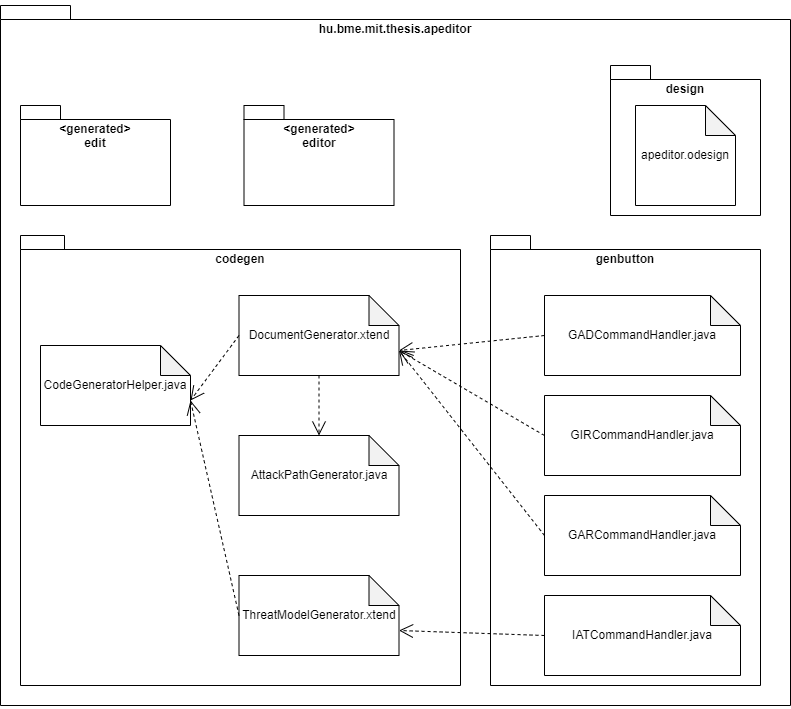
\includegraphics[width=130mm, keepaspectratio]{figures/05_package_apeditor.png}
	\caption{APEditor projekt felépítése és dependenciái}
	\label{fig:05_apeditor_arch}
\end{figure}

A \textbf{hu.bme.mit.thesis.apeditor} projektben található az \textit{apeditor.ecore} fájl ami a metamodellt tartalmazza, illetve az Eclipse Modelling Framework által generált fájlokat.

A \textbf{hu.bme.mit.thesis.apeditor.edit} illetve a \textbf{hu.bme.mit.thesis.apeditor.editor} projektek szintén az EMF által lettek generálva, ezek adják meg a modell szerkesztő felületének az alapjait.

A \textbf{hu.bme.mit.thesis.apeditor.design} tartalmaz egy Sirius keretrendszert használó \textit{apeditor.odesign} fájlt amely a támadási fáknak a grafikus megjelenítését és szerkesztő felületét írja le.

A \textbf{hu.bme.mit.thesis.apeditor.genbutton} tartalmazza a plugin.xml-t amelyben az APEditor felhasználói felületén megjelenítendő gombok vannak leírva, valamint a gombok megnyomásával futtatott .java fájl is itt kerül összelinkelésre. A négy .java fájl a különböző funkcionalitását definiálják.

\begin{itemize}
	\item \textbf{GADCommandHandler.java} Asset Definition workproduct generálását viszi véghez a \textbf{hu.bme.mit.thesis.apeditor.codegen} projektben definiált funkcionalitás aktiválásával
	\item \textbf{GIRCommandHandler.java} Impact Rating workproduct generálását viszi véghez a \textbf{hu.bme.mit.thesis.apeditor.codegen} projektben definiált funkcionalitás aktiválásával
	\item \textbf{GARCommandHandler.java} Attack Feasibility Rating workproduct generálását viszi véghez a \textbf{hu.bme.mit.thesis.apeditor.codegen} projektben definiált funkcionalitás aktiválásával
	\item \textbf{IATCommandHandler.java} Inicializálja a támadási fákat az \textbf{hu.bme.mit.thesis.apeditor.codegen} projektben definiált funkcionalitás aktiválásával
\end{itemize} 

Végül az \textbf{hu.bme.mit.thesis.apeditor.codegen} tartalmazza a kódgeneráláshoz szükséges osztályokat és függvényeket. Itt egyrészről a \textit{DocumentGenerator.xtend} fájl tartalmazza azokat az Xtend-ben megírt függvényeket, amelyek a szabványos workproduct-ok előállításához szükségesek, másrészről az Attack Feasibility Rating generálásakor, használja az \textit{AttackPathGenerator.java} függvényeit amelyek a támadási fákat fejti ki támadási útvonalakká amelyek támadási lépésekből állnak.

Az \textit{ThreatModelGenerator.xtend} a modellből generálja le a támadási fák kezdeti állapotát és aztán azokat írja bele a modellfájlba. Ezzel bővítve a szerkesztett modellt.

Mindkét Xtend fájl a \textit{CodeGeneratorHelper.java} fájlt használja még a fájlba író és fájlt olvasó műveletek elvégzésére.

\subsection{Metamodel}

\begin{figure}[!ht]
	\centering
	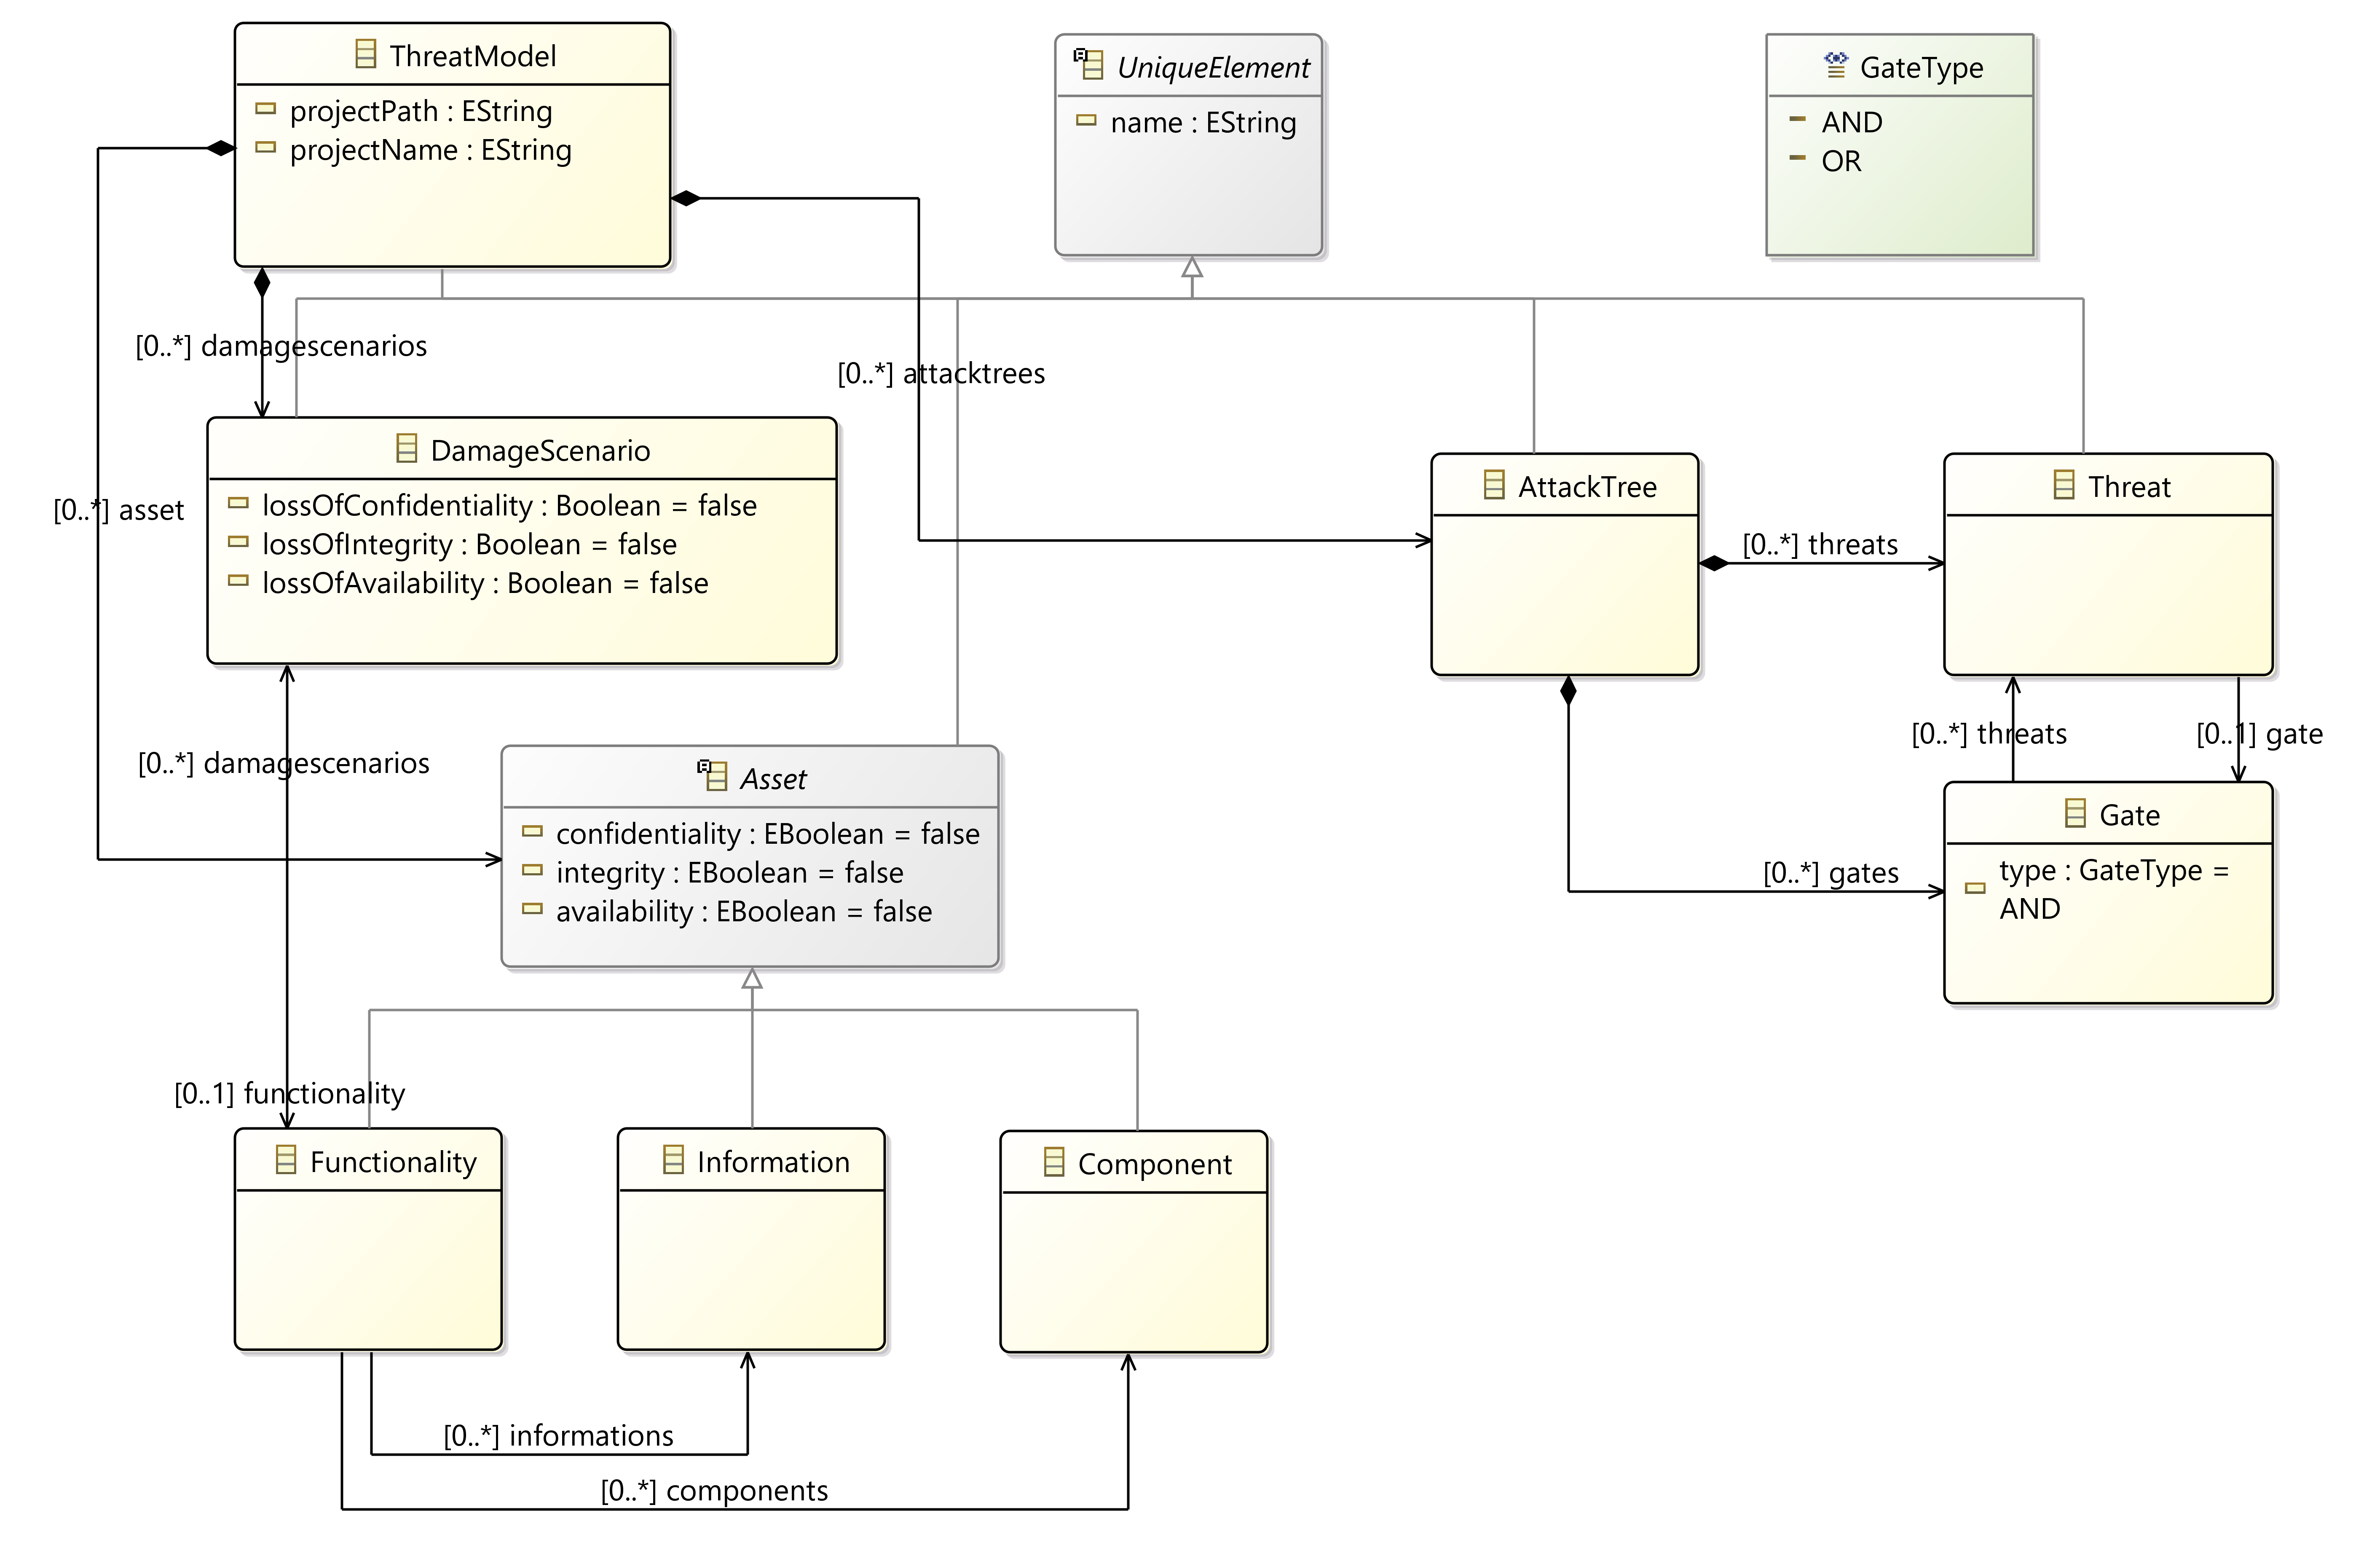
\includegraphics[width=130mm, keepaspectratio]{figures/05_metamodel.png}
	\caption{apeditor.ecore fájlban definiált metamodell}
	\label{fig:05_metamodel}
\end{figure}

\subsection{Fenyegetésmodell szerkesztő felület}

\subsection{Támadási fák inicializálása}

\subsection{Támadási fa szerkesztő felület}

\subsection{Dokumentum generátor}
\chapter{Esettanulmány}

Az esettanulmányomnak a célja, hogy egy példán keresztül bemutassam az általam fejlesztett elemző eszköz valamint a rendszermodellből való származtatásnak a folyamatát.

Az esettanulmányom tárgyaként az elektronikus vezérlő egységek (ECU) diagnosztikai szolgáltatását választottam. Ennek oka egyrészről az, hogy az elemzett diagnosztikai szolgáltatások specifikációja publikusan elérhető az ISO 14229 "Road vehicles - Unified Diagnostic Services (UDS)" \cite{ISO14229} szabványban. Másrészről ez egy olyan potenciális belépőpontja lehet a támadóknak amely nem igényel semmiféle fizikai hozzáférést a járműhöz. Amennyiben távolról sikeresen hozzáfér és átveszi az irányítását a támadó egy elektronikus vezérlő egységnek, ami képes V2X vagy más vezetéknélküli szolgáltatásra, onnantól kezdve a jármű többi részén lévő diagnosztikai szolgáltatások is elérhetővé válhatnak számára.\\

Az ISO 14229 \cite{ISO14229} definiálja az Unified Diagnostic Services (röviden UDS) protokollt ami egy alkalmazásrétegbeli szolgáltatás. Általános IT biztonsági szempontból, ehhez legközelebbinek a TLS és HTTPS protokollok lennének mondhatók.

\begin{figure}[!ht]
	\centering
	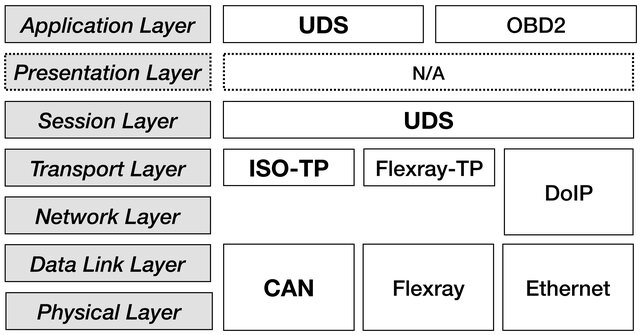
\includegraphics[width=120mm, keepaspectratio]{figures/06_isoosi.jpg}
	\caption{ISO/OSI modell autóipari kommunikációs protokollokra \cite{ISOOSI}}
\end{figure}

Az esettanulmányomban a szolgáltatások közül kettővel, a diagnosztikai autentikációval, valamint a software frissítéssel fogok foglalkozni, mivel ezek a kiemelten kiberbiztonsági relevanciával rendelkező szolgáltatások.\\

A diagnosztikai autentikációt két módon lehet implementálni. Az egyik a \textbf{Security Access (0x27)} a másik pedig a korszerűbb \textbf{Authentication (0x29)} lenne. 

A \textbf{Security Access}-szel az úgynevezett challange-response autentikációt lehet megvalósítani, amelynek a menete először egy valamilyen ismeretlen ECU-n belüli információnak (\textit{seed}) a szolgáltatása a diagnosztikai tesztelő részére, aki ezt az információt valamilyen közös titok (pl: szimmetrikus kulcs) használatával előállít egy kulcsot, amelyet elküld az ECU-nak. Az ECU a fogadó oldalon ellenőrzi, hogy a kulcs ami érkezett az megegyezik azzal amit ugyanezen közös titok és algoritmus használatával állított elő a \textit{seed} lekérése után. Amennyiben a kulcsok megegyeznek az ECU a felhasználót átengedi magasabb biztonsági szinthez ezzel hozzáférést biztosítva korábban nem elérhető diagnosztikai szolgáltatásokhoz.

Az \textbf{Authentication} már egy jóval komplexebb, tanúsítvány alapú autentikációt tesz lehetővé. Ennek a bemutatása túl mutat a jelen esettanulmányon.\\

A szoftverfrissítés egy több lépésből álló szekvenciája diagnosztikai rutin hívásoknak, amelyeket a szabvány "Upload download functional unit" fejezetében fejt ki.

Annak a folyamata, hogy egy új szoftver kerüljön fel az ECU-ra jellemzően a következő lépésekből áll:
\begin{itemize}
	\item \textbf{RequestDownload (0x34)}: Előfeltételek ellenőrzése, letöltési kérelem jóváhagyása
	\item \textbf{TransferData (0x36)}: Adatok feltöltése
	\item \textbf{RequestTransferExit (0x37)}: Érkezett adatok ellenőrzése, jóváhagyás, szoftver indíthatóvá tétele
\end{itemize}

Ezt a folyamat természetesen bővíthető további vagy ezeket megelőző lépésekkel, illetve az egyes rutinok belső működése sincs szabályozva. Maga a kerete viszont egy szoftverfrissítésnek az jellemzően ilyen diagnosztikai szolgáltatások futtatásával és kérések kiszolgálásával történnek az elektronikus vezérlőegységeken.

Érdemes kiemelni itt, hogy ez a frissítési metódus eleinte a járműszervizben történt volna a szerelő által, de a napjainkban már ezeknek a távoli elérése, jellemzően egy külön erre integrált elektronikus vezérlőegység által is lehet lefolytatva. Ezeknek sokban kényelmi, de szintén szoftveres sérülékenységek vagy hibák javítása szempontjából is fontos szerepük van.\\

A protokoll egyébként tartalmaz olyan szolgáltatásokat mint a \textbf{Routine Control (0x31)} amellyel a beszállító és a vevő az eszközre specifikus, nem szabványos diagnosztikai szolgáltatásokat is definiálhat. Ilyenek lehetnek kulcs és tanúsítványkezelő rutinok, illetve gyártósoron használt szolgáltatások.

\section{Károkozások és értékek azonosítása}

A \ref{fig:diag_abuse} ábrán láthatóak a potenciális károkozások. A korábban meghatároztuk a két fő szolgáltatást ami az esettanulmányban elemzésre kerül, majd ezekhez a CIA triád mentén való elemzés szerint meghatározásra kerültek a potenciális károkozások. Továbbá egy egy azonosító is került a károkozások nevébe, valamint a felvett sztereotípiával az attributálást is el lehetett végezni.

\begin{itemize}
	\item \textbf{DS-SECDIAG-00 Leak confidential data}: Amennyiben az autentikációs szolgáltatás bizalmassága elveszik, abban az esetben a támadónak lehetősége lesz a bizalmas diagnosztikai adatok kiolvasására
	\item \textbf{DS-SECDIAG-01 Acces unauthorized functionality}: Az autentikációs szolgáltatás integritásának a megtörése vezethet olyan szolgáltatások elérhetővé válásához amelyek normális esetben nem lennének elérhetőek
	\item \textbf{DS-SECDIAG-02 Block authentication attempts}: Az autentikációs szolgáltatás elérhetőségének a blokkolásával korlátozható jogosult felhasználóknak a korlátozott szolgáltatásokhoz való hozzáférése
	\item \textbf{DS-SECSW-00 Leak software}: A szoftver kiszivárogtatásával lehetőség adódik a szoftverben sérülékenységek keresésére, annak kihasználását könnyebbé téve
	\item \textbf{DS-SECSW-01 Change software}: A szoftver megváltoztatásával kártékony szoftver is feljuttatható az elektronikus vezérlőegységre
	\item \textbf{DS-SECSW-02 Remove software}: A szoftver elérhetőségének korlátozásával az elektronikus vezérlőegység teljes funkcionalitása blokkolhatóvá tehető
\end{itemize}

\begin{figure}[!ht]
	\centering
	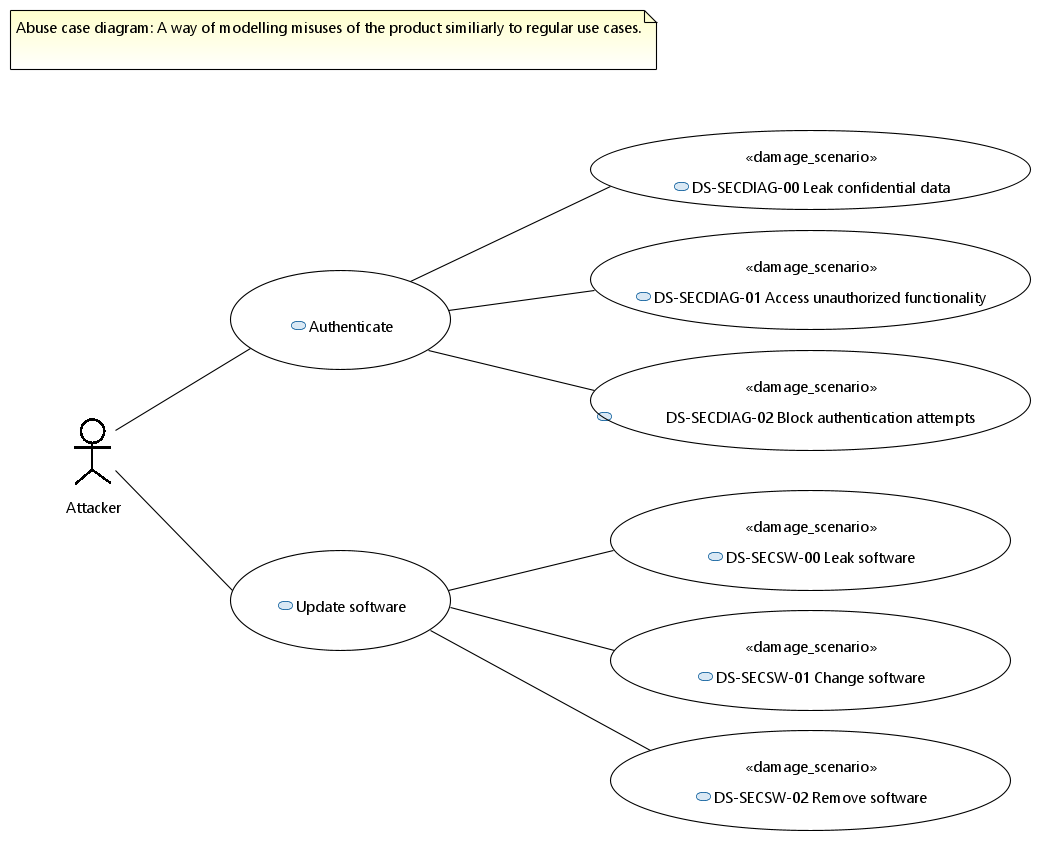
\includegraphics[width=120mm, keepaspectratio]{figures/06_01_abuse_case_diagram.PNG}
	\caption{Diagnosztika kihasználási esetei}
	\label{fig:diag_abuse}
\end{figure}

A termékleíráshoz a funkcionalitásokat definiáltuk, kellenek még az ezek által dependált értékek. HW-es komponensből egyedül a CAN csatlakozó hozható fel hiszen azon fog keresztül utazni a bejövő UDS üzenet. SW-szintű értékekből vehetjük a CAN üzenetet amiben utazik az UDS üzenet, maga az UDS üzenet, valamint az az által szállított adatok. Ez a szállított adat a szoftverfrissítés esetén a szoftver lesz, egyébként pedig diagnosztikai adatok lehetnek elérhetőek kiolvasásra az autentikációt követően.

A termékleírás ábrázolva a \ref{fig:item_def} ábrán látható. A sztereotípiák felvétele után volt lehetőségem az attributálásra, ezt a következőképpen tettem meg:
\begin{itemize}
	\item \textbf{Diagnostic Authentication}: A károkozásokból származtathatóan a CIA minden tulajdonsága vonatkozik a funkcionalitásra
	\item \textbf{Software Update}: A károkozásokból származtathatóan a CIA minden tulajdonsága vonatkozik a funkcionalitásra
	\item \textbf{CAN Connector}
	\subitem Sértetlenség: Egy CAN csatlakozó integritását megsértve, kártékony eszközökkel kerülhet kapcsolatba az elemzés tárgyaként szereplő ECU
	\subitem Elérhetőség: Egy CAN csatlakozó elérhetőségét megsértve, a beérkező üzenetek hiányára kell felkészülni
	\item \textbf{CAN Message}
	\subitem Bizalmasság: Az üzenet tartalmazhat bizalmas információt amely segíthet további támadások esetén
	\subitem Sértetlenség: Az üzenet tartalma változtatható, ezzel a fogadó félnél kiváltott reakció is
	\subitem Elérhetőség: Az üzenet blokkolható, a hiánya a fogadó félnél nem zárható ki
	\item \textbf{UDS Message}
	\subitem Bizalmasság: Az üzenet tartalmazhat bizalmas információt amely segíthet további támadások esetén
	\subitem Sértetlenség: Az üzenet tartalma változtatható, ezzel a fogadó félnél kiváltott reakció is
	\subitem Elérhetőség: Az üzenet blokkolható, a hiánya a fogadó félnél nem zárható ki
	\item \textbf{Software}
	\subitem Bizalmasság: A szoftver a fejlesztő cég szellemi tulajdona, ennek kiszivárgása egyrészről anyagi kárt, másrészről további támadások elvégzését is segítheti
	\subitem Sértetlenség: A szoftver változtatható, ezzel a futtató ECU működése is
	\subitem Elérhetőség: A szoftver törölhető, hiánya az ECU biztonságos működését befolyásolhatja
	\item \textbf{Diagnostic Data}
	\subitem Bizalmasság: Az üzenet tartalmazhat bizalmas információt amely segíthet további támadások esetén
\end{itemize}

\begin{figure}[!ht]
	\centering
	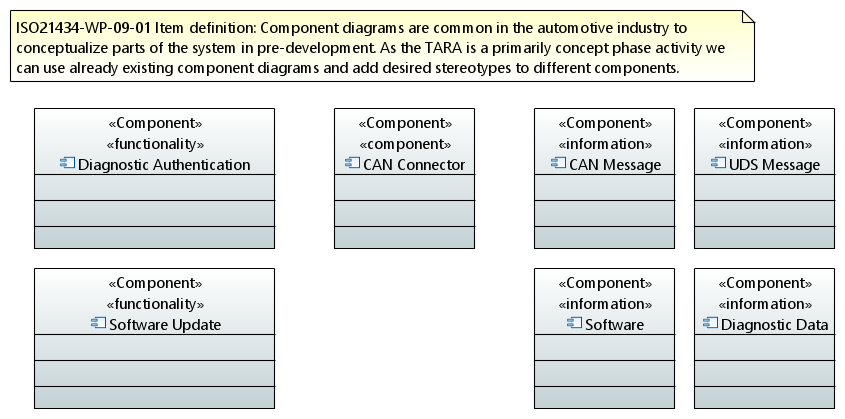
\includegraphics[width=120mm, keepaspectratio]{figures/06_02_item_definition_diagram.PNG}
	\caption{Diagnosztika termékleírása}
	\label{fig:item_def}
\end{figure}

\section{Fenyegetésmodell származtatása}

Az Acceleo szkript futtatása a következő fájlt hozza létre Diagnostics.apeditor néven:

\begin{lstlisting}[basicstyle=\tiny]
<apeditor:ThreatModel xmi:version="2.0" xmlns:xmi="http://www.omg.org/XMI" xmlns:xsi="http://www.w3.org/2001/XMLSchema-instance" xmlns:apeditor="hu.bme.mit.thesis.apeditor">
<damagescenarios name="DS-SECSW-00 Leak software" lossOfConfidentiality="true" lossOfIntegrity="false" lossOfAvailability="false"/>
<damagescenarios name="DS-SECSW-01 Change software" lossOfConfidentiality="false" lossOfIntegrity="true" lossOfAvailability="false"/>
<damagescenarios name="DS-SECSW-02 Remove software" lossOfConfidentiality="false" lossOfIntegrity="false" lossOfAvailability="true"/>
<damagescenarios name="DS-SECDIAG-00 Leak confidential data" lossOfConfidentiality="true" lossOfIntegrity="false" lossOfAvailability="false"/>
<damagescenarios name="DS-SECDIAG-01 Access unauthorized functionality" lossOfConfidentiality="false" lossOfIntegrity="true" lossOfAvailability="false"/>
<damagescenarios name="DS-SECDIAG-02 Block authentication attempts" lossOfConfidentiality="false" lossOfIntegrity="false" lossOfAvailability="true"/>
<asset xsi:type="apeditor:Functionality" name="Software Update"/>
<asset xsi:type="apeditor:Functionality" name="Diagnostic Authentication"/>
<asset xsi:type="apeditor:Component" name="CAN Connector" confidentiality="false" integrity="true" availability="true"/>
<asset xsi:type="apeditor:Information" name="CAN Message" confidentiality="true" integrity="true" availability="true"/>
<asset xsi:type="apeditor:Information" name="UDS Message" confidentiality="true" integrity="true" availability="true"/>
<asset xsi:type="apeditor:Information" name="Software" confidentiality="true" integrity="true" availability="true"/>
<asset xsi:type="apeditor:Information" name="Diagnostic Data" confidentiality="true" integrity="false" availability="false"/>
</apeditor:ThreatModel>
\end{lstlisting}

\section{Fenyegetésmodellezés}

A generált fájl innentől beimportálható és megnyitható olyan Eclipse környezettel amelyhez az elemzőeszköz plugin fájljai hozzá vannak adva.

A dependenciák meghatározásánál a károkozásokhoz hozzátudjuk rendelni a funkcionalitást viszonylag egyértelműen, maga az azonosítójuk is jelzi melyik károkozás melyik funkcióhoz tartozik.

Továbbá mindkét funkcionalitáshoz tartozik a \textbf{CAN Connector} mint HW komponens valamint a \textbf{CAN Message} és \textbf{UDS Message} mint információ. Amiben a két funkcionalitás eltér, hogy ameddig a \textbf{Software Update} esetén az érkező üzenetek a \textbf{Software}-t tartalmazzák, addig az autentikáció után elsősorban a kimenő \textbf{Diagnostic Data} az érték amit védeni akarunk.

Ebből generált majd megszerkesztett hibafák és elemzésük alább megtekinthető. \\
\newpage

\section{Támadási fa analízis}

Ahogy az a \ref{fig:ff_leak_sw} ábrán látható a gyökér fenyegetés a \textbf{Software Update} bizalmasságának sértését okozó \textit{Disclosure of Software Update} lesz. Ez azt jelenti, hogy ezt a funkcionalitást vagy az ehhez tartozó diagnosztikai rutinokat olyan módon használják amellyel bizalmas információkhoz juthat a támadó.

Először levontam a következtetést, hogy egyrészről minden lehetséges támadás azzal fog kezdődni, hogy a támadó valahogyan sérti az integritását a CAN busznak vagy a rendszer csatlakozóján vagy az ahhoz kapcsolódó elemek módosításával. Ez jelenthet fizikai hozzáférést vagy amennyiben egy csatlakoztatott eszköz felett szerez irányítást a támadó, abban az esetben ez akár távolról is elvégezhető.

Másodsorban két támadási irányt különítettem el, az egyik esetben a támadó megpróbál olyan diagnosztikai szolgáltatásokat használni amelyekkel a telepített szoftver kinyerhető lenne az eszközből. A másik esetben az éppen folyamatban lévő szoftverfrissítésnél érkező üzenetek lehallgatásával és azok tartalmának visszafejtésével próbálhat a támadó a szoftverhez hozzájutni. Előbbi esetben egy CAN üzenet lehallgatásával (disclosure) hozzájut a CAN ID-khoz és paraméterekkel, majd módosított üzeneteket injektál amelyekkel a szoftver letöltését kezdeményezheti. A másik esetben UDS üzenet lehallgatás és a szoftver visszafejtése történne.

\begin{figure}[!ht]
	\centering
	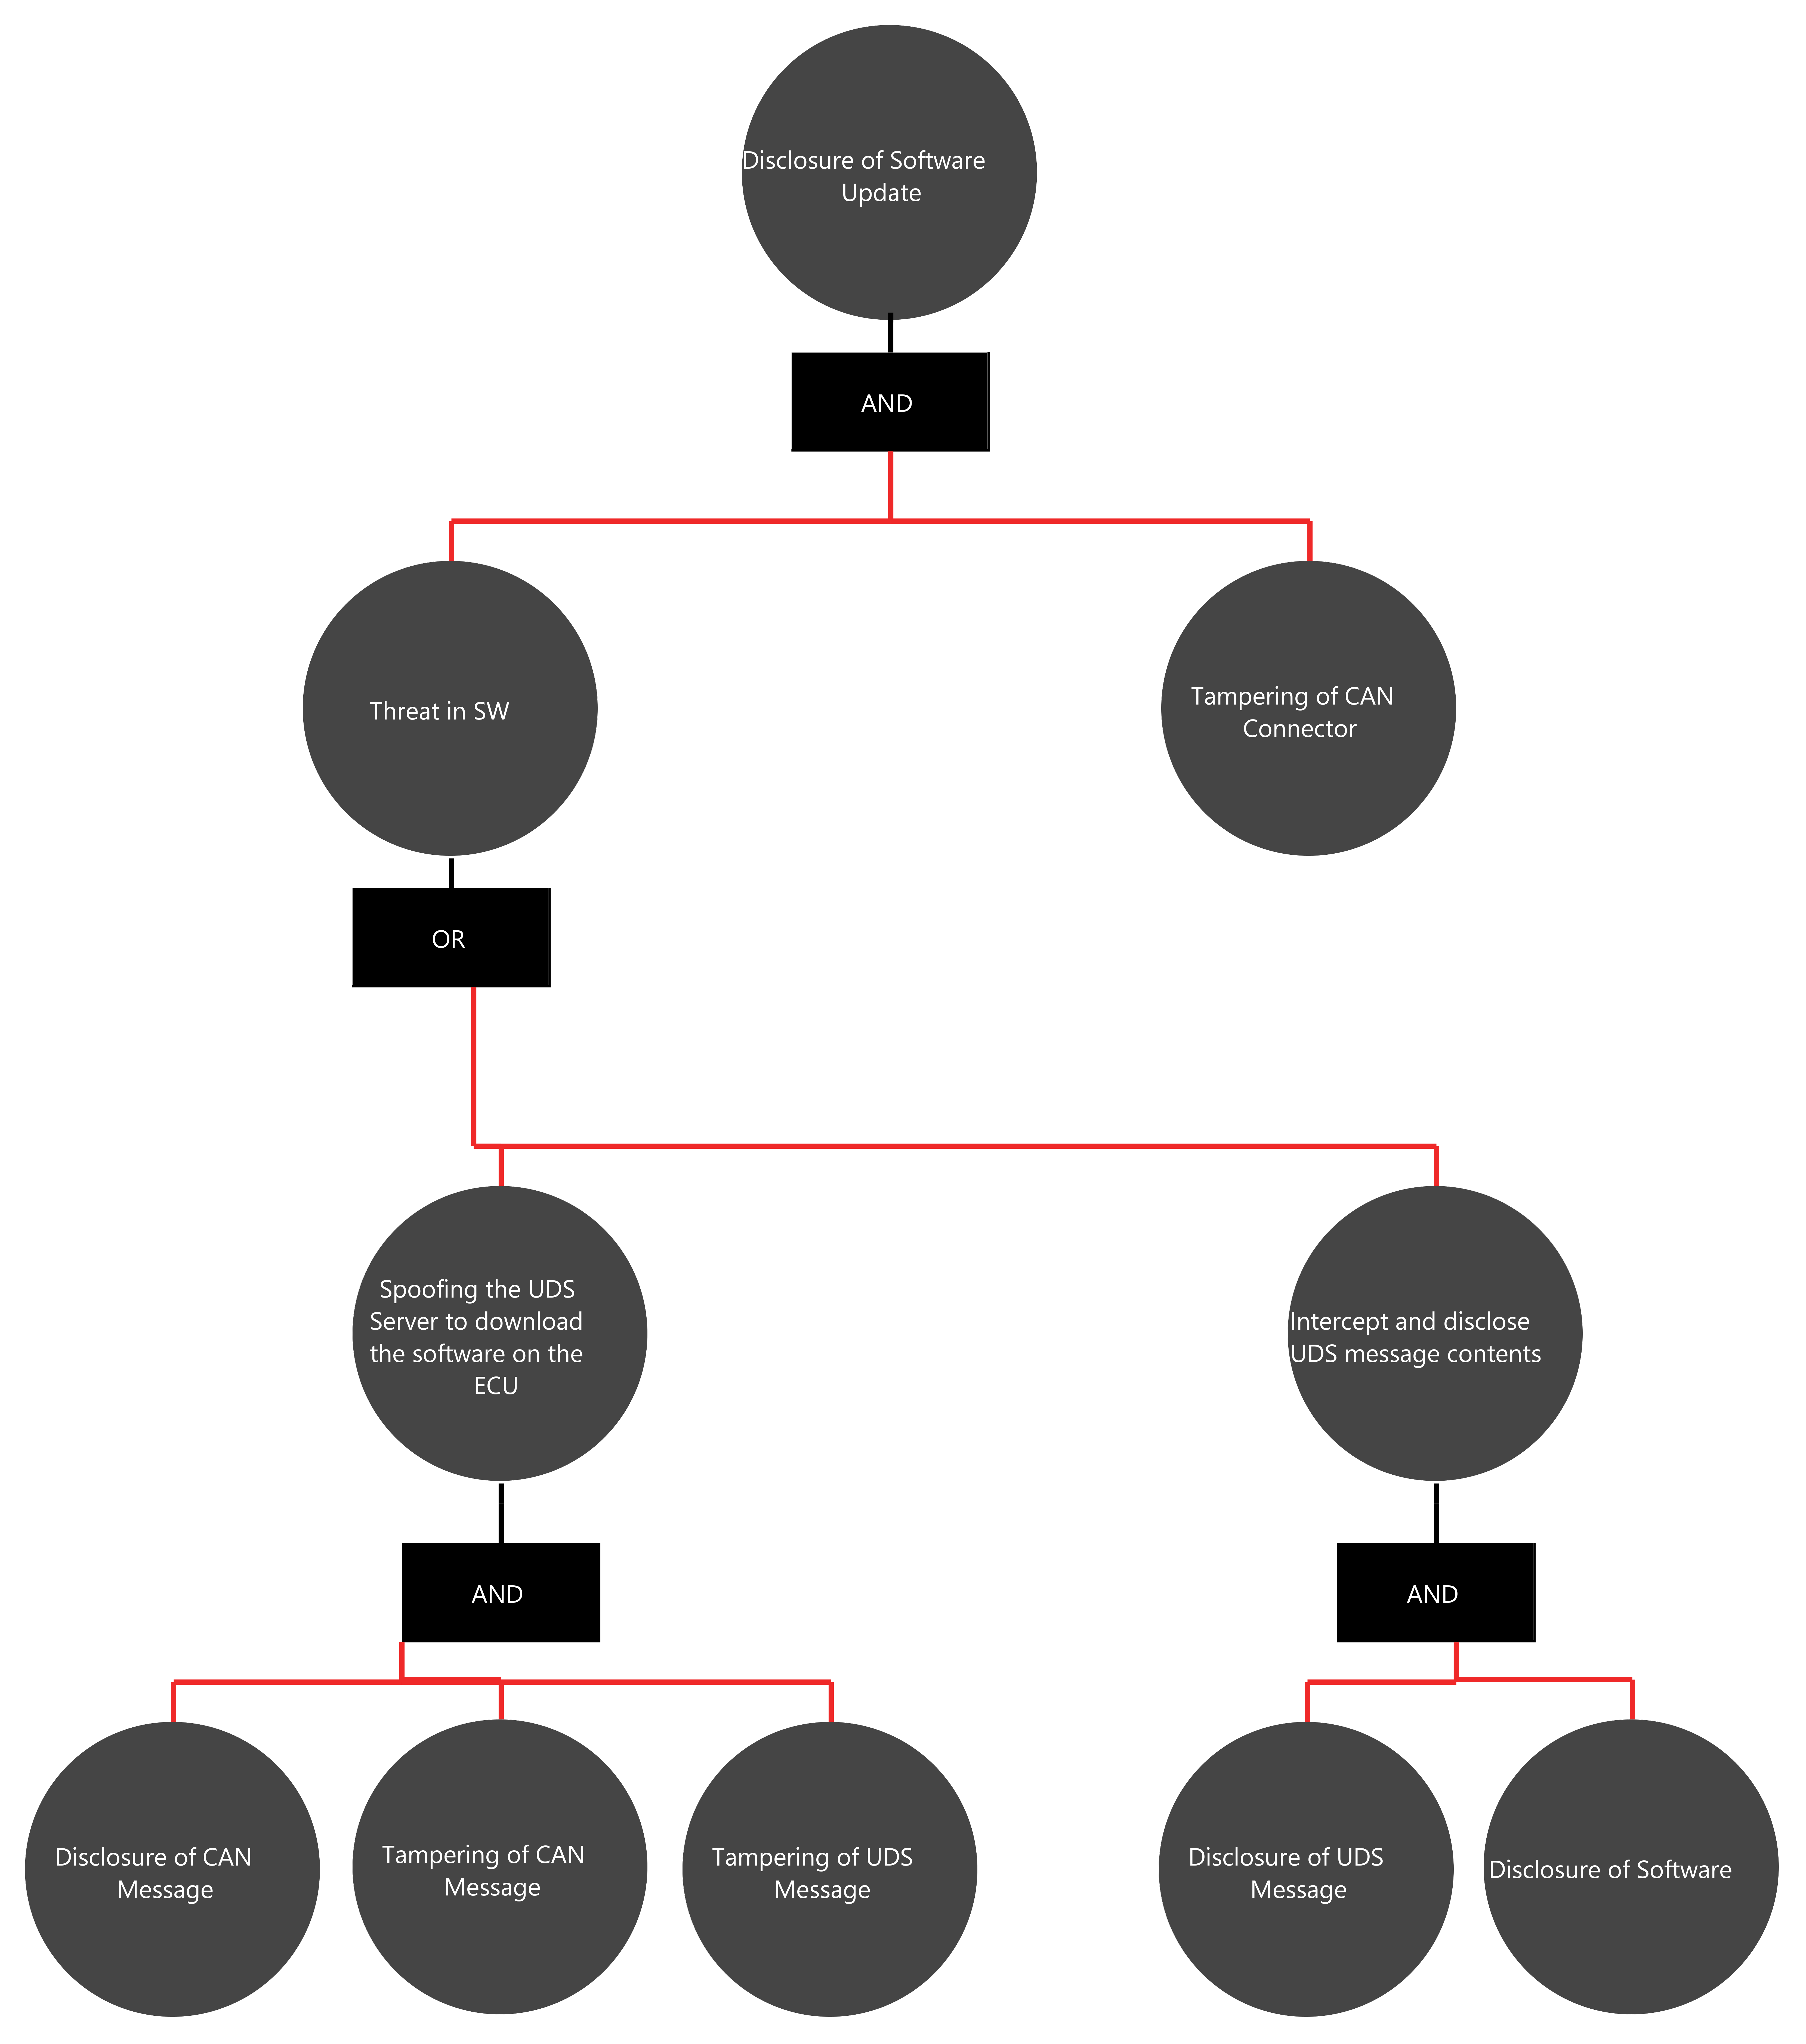
\includegraphics[width=120mm, keepaspectratio]{figures/AT-SECSW-00.png}
	\caption{Támadási fa a "Leak software" károkozáshoz} 
	\label{fig:ff_leak_sw}
\end{figure}

\newpage

A következő támadási fa a \textit{Change software} károkozáshoz készült és az \ref{fig:ff_change_sw} ábrán látható. 

Itt egyrészről különvettem egy \textit{Surveillance} pszeudo-fenyegetést, amely maga alá gyűjti azokat a fenyegetéseket amelyek önmagukban nem képesek a károkozást okozni, azonban ezt is kénytelenek előzetesen megtenni. A feltételezés az az, hogy a támadónak egy szoftver frissítési folyamatot le kell hallgatnia ahhoz, hogy a sajátját is véghez vigye. Itt egyrészről arról van szó, hogy a támadó azonosítja az ECU-kat a CAN és UDS üzenetek metaadatai alapján, valamint a szoftver felépítését is szükséges azonosítania ahhoz, hogy végül egy saját szoftvert is képes legyen az eszközre feltölteni.

Emellett egyértelműen szükséges a HW oldaláról a CAN busz integritásának megváltoztatása, hogy a támadó képes legyen a saját üzeneteit elküldeni a célpont ECU-nak.

Végül maga a szerkesztett vagy saját szoftver feltöltés lesz a következő lépés, ez magával vonja mind az egyedi CAN és UDS üzenet illetve szoftver létrehozását a támadó oldalról, úgy, hogy azt a célpont ECU elfogadja.

Megfigyelhető, hogy itt egyébként nincs szükség erre a szegmentálásra, hiszen minden atomi fenyegetésnek jelen kell lennie a rendszerben a rendszerszintű fenyegetés aktiválásához, viszont ebben a formában átláthatóbb és funkcionálisan nincs hatással az elemző eszköz működésére ez a formátum.

\begin{figure}[!ht]
	\centering
	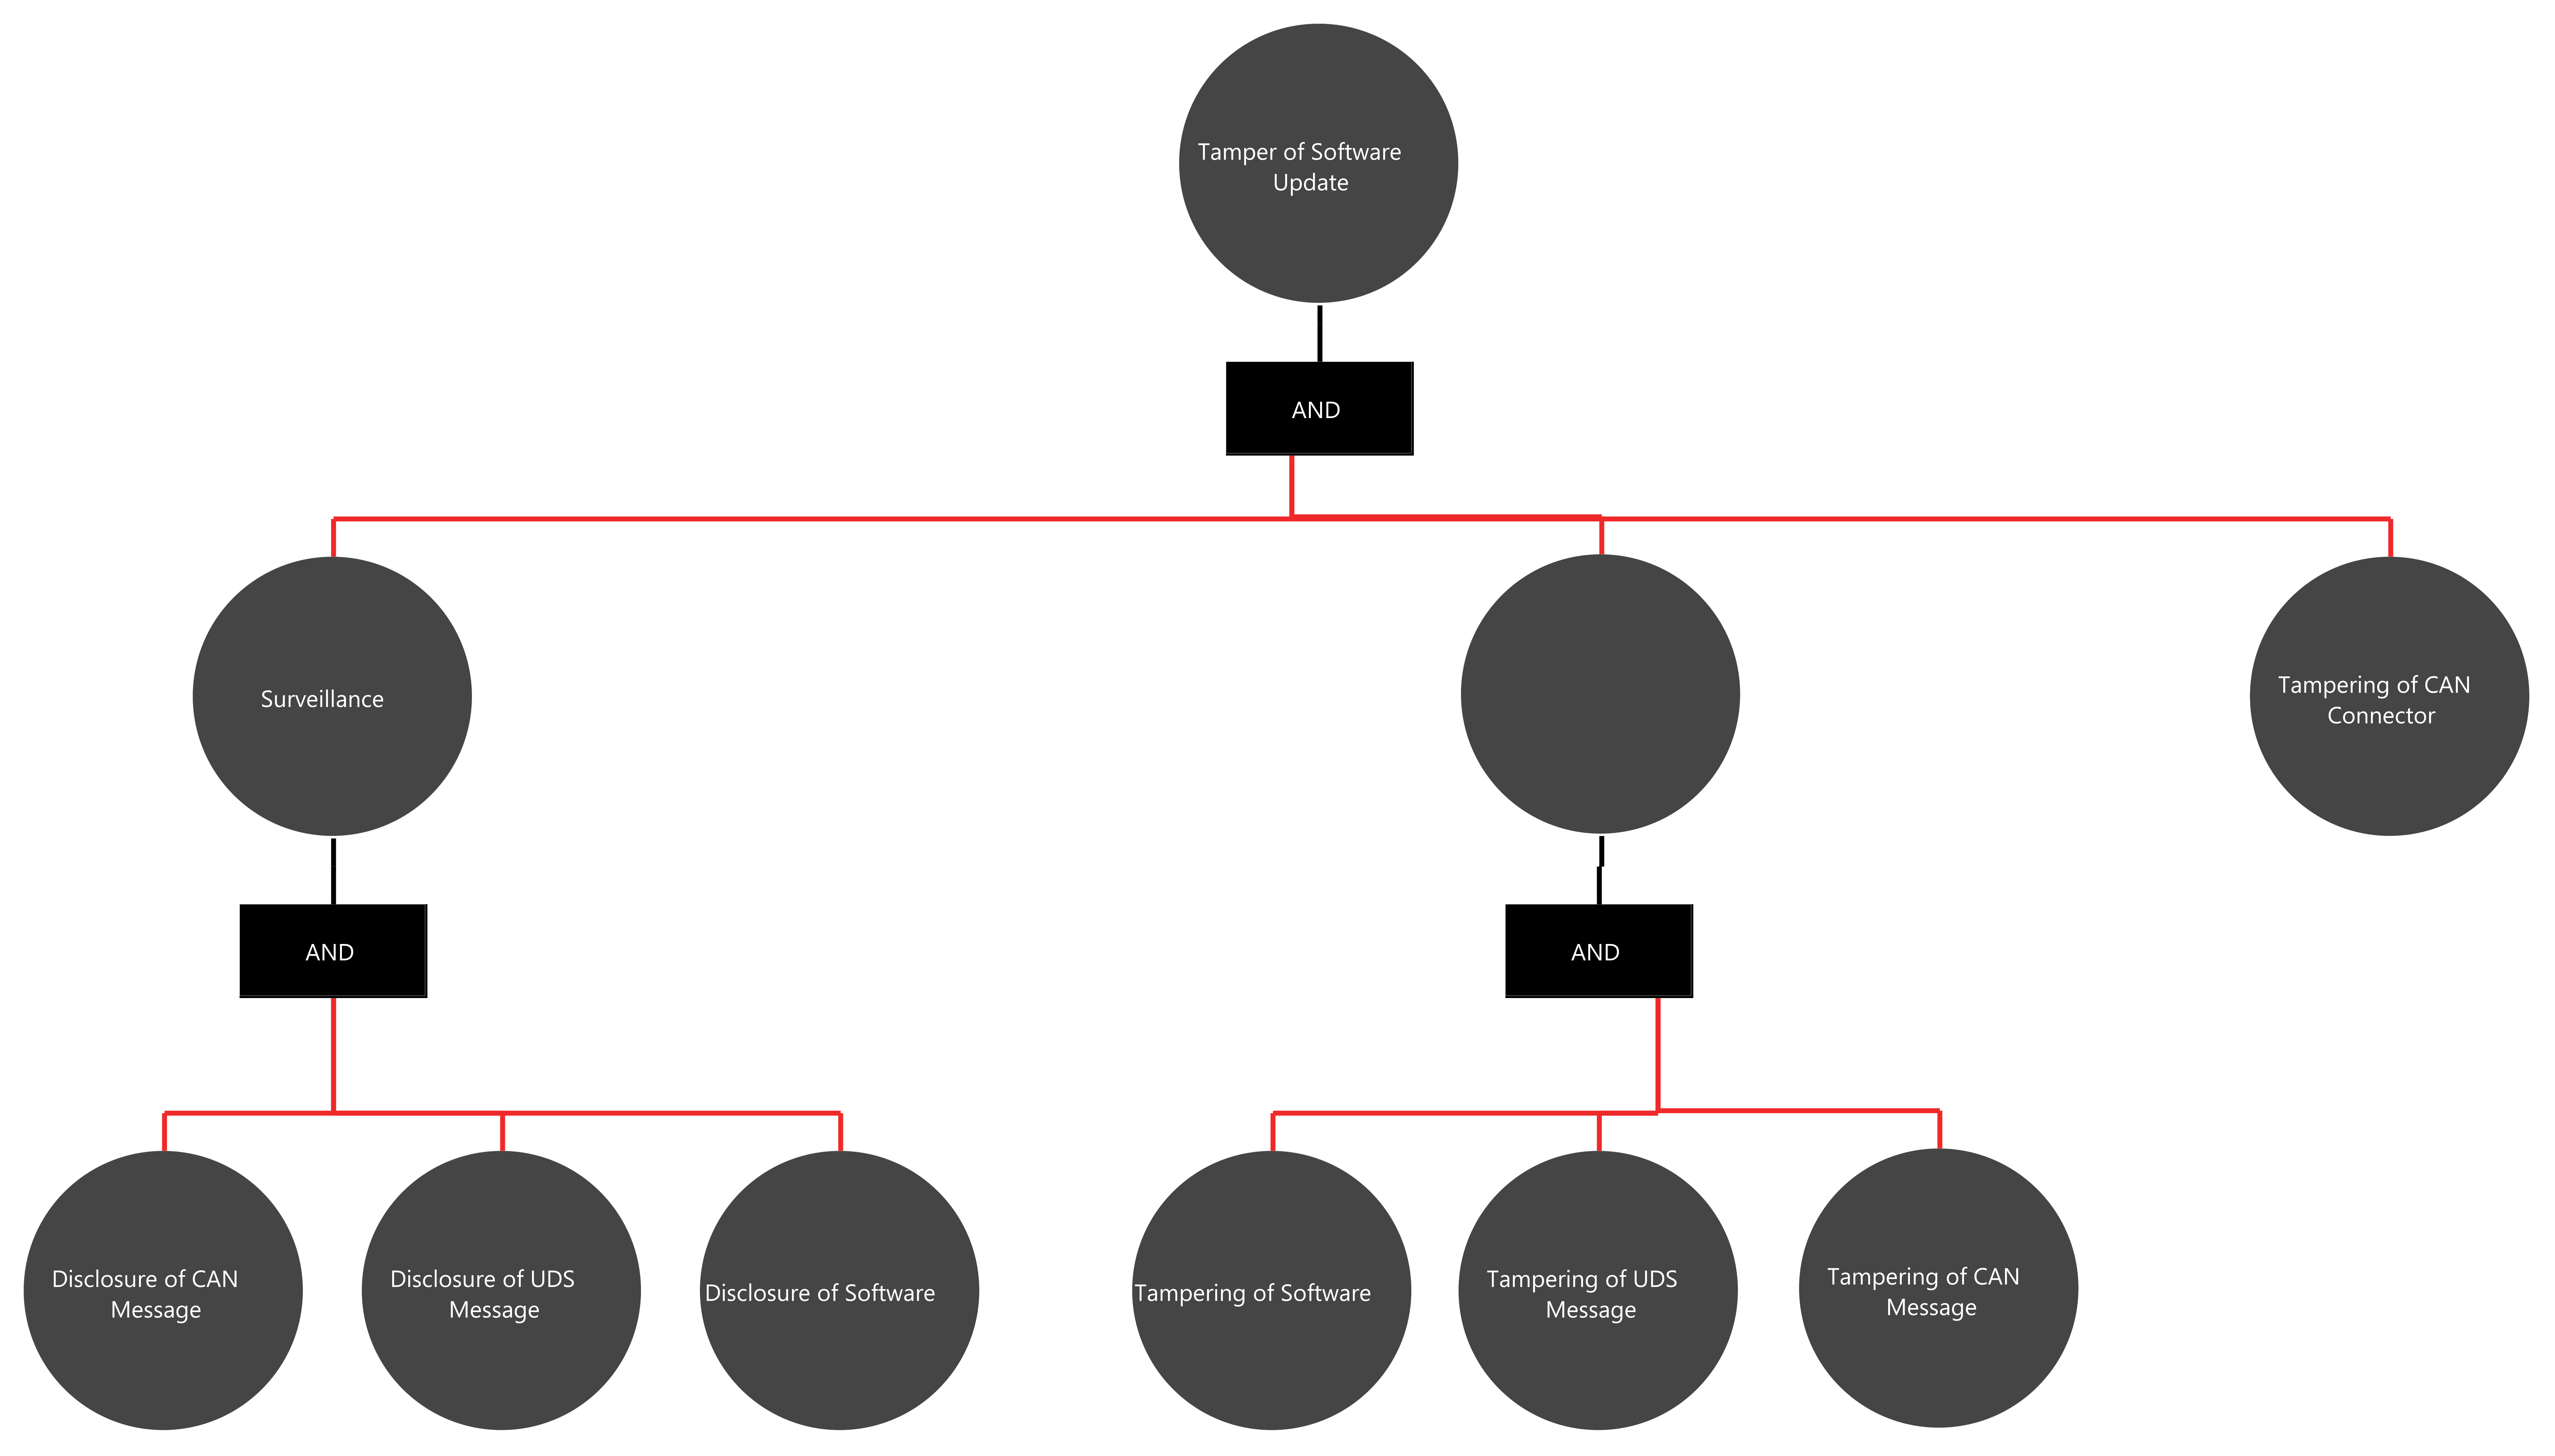
\includegraphics[width=120mm, keepaspectratio]{figures/AT-SECSW-01.png}
	\caption{Támadási fa a "Change software" károkozáshoz} 
	\label{fig:ff_change_sw}
\end{figure}

\newpage

A szoftver elérhetőségének módosítására az \ref{fig:ff_remove_sw} ábrán láthatjuk a támadási fát. Ez a támadás már sokkal több módon elvégezhető, a kár kisebb a többi esethez képest azonban az elvégzéséhez szükséges tudás is a támadó részéről.

Egyrészről az első szinten külön vettem a HW-es kapcsolat megszüntetését amely egy fizikai hozzáférést jelentene a járműhöz attól ami potenciálisan távolról is elvégezhető.

A távolról elvégezhető esetben lehetőség szerint a támadó egyrészről sértenie kell a CAN busz integritását másrészről vagy az érkező üzenetek blokkolását kell elérnie, ezzel a szoftver funkcionalitását blokkolva vagy azokat úgy módosítva, hogy utána a célpont ECU ne fogadja el azokat (pl. szálított adat módosítása úgy hogy a CRC nincs módosítva egyenesen vezetne az üzenet eldobásához üzembiztonsági elvárások miatt).

\begin{figure}[!ht]
	\centering
	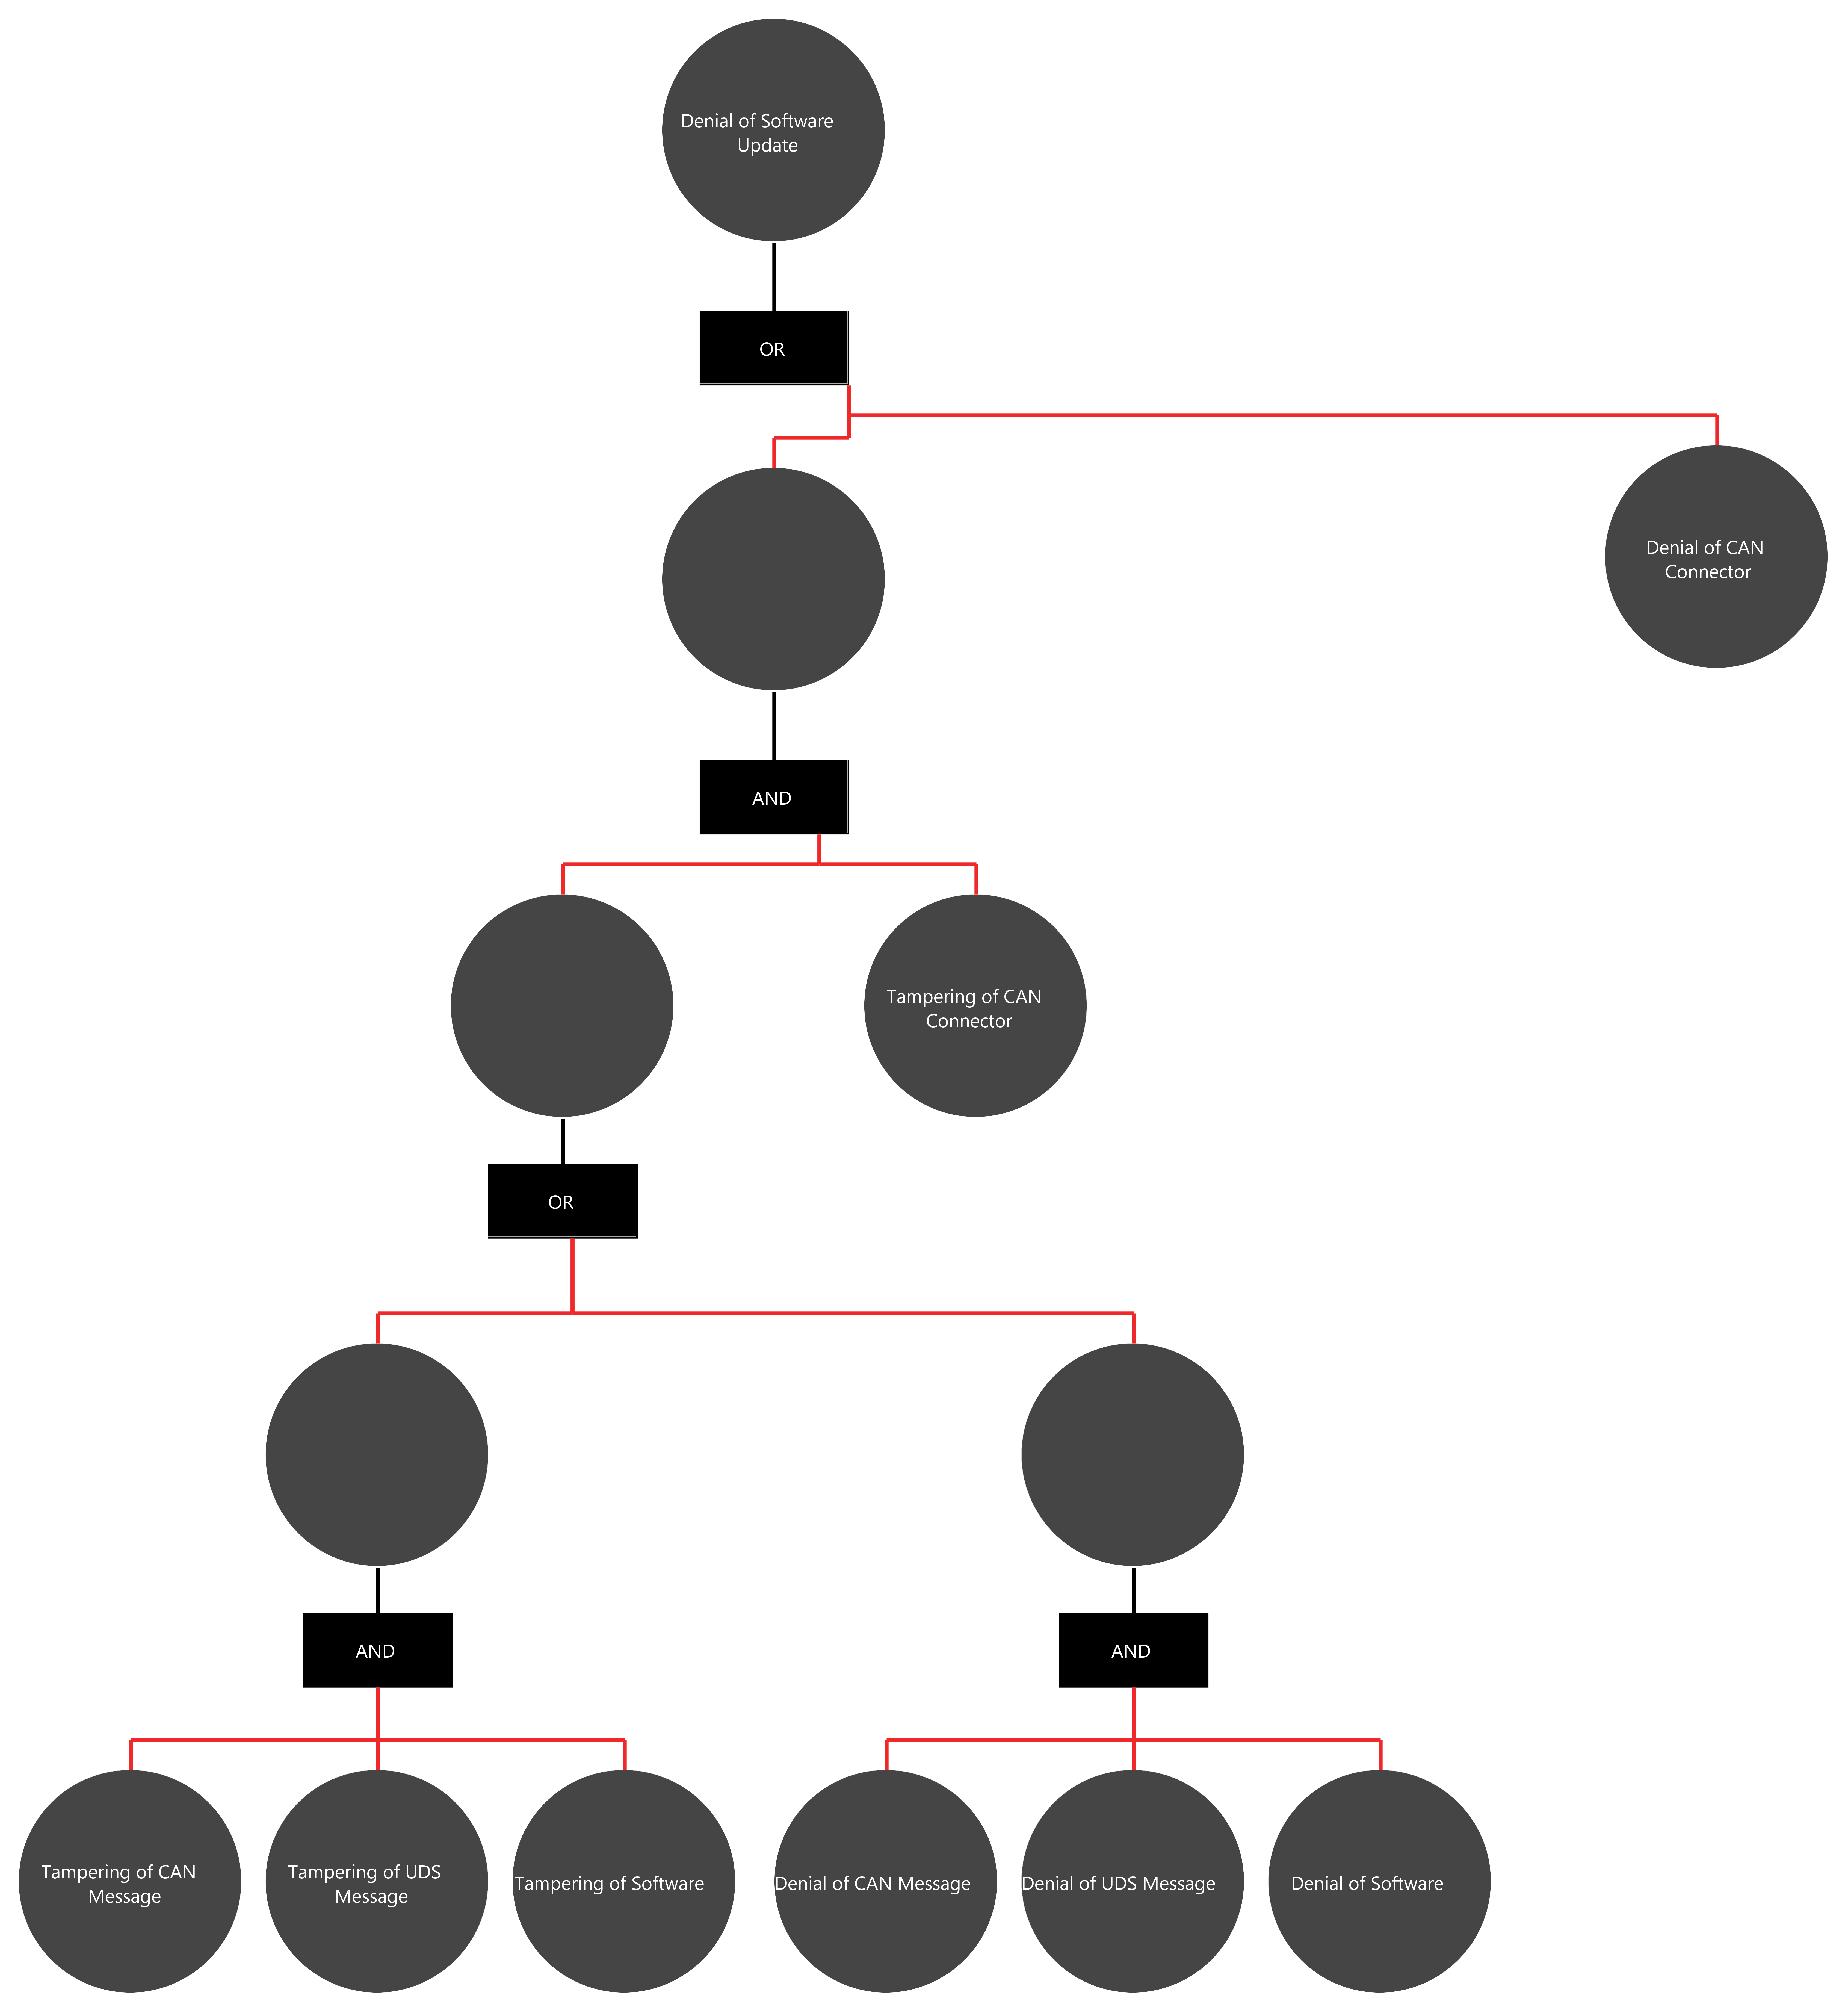
\includegraphics[width=120mm, keepaspectratio]{figures/AT-SECSW-02.png}
	\caption{Támadási fa a "Remove software" károkozáshoz} 
	\label{fig:ff_remove_sw}
\end{figure}

\newpage

Áttérve a diagnosztikai adatok szivárogtatására az \ref{fig:ff_leak_data} ábrán, itt is alapvetésnek vesszük a CAN busz integritásának változását valamint magát az adatszivárgást.

A következő szinten két utat különböztetünk meg az információkhoz való hozzáférésnél, egyik esetben a bejövő üzenetek lehallgatása és visszafejtése lehet a támadó megoldása. A másik bonyolultabb esetben olyan üzeneteket kell a támadónak konstruálnia amelyeket a célpont ECU tud értelmezni valamint, megfelelőnek és jogosultnak ítél.

\begin{figure}[!ht]
	\centering
	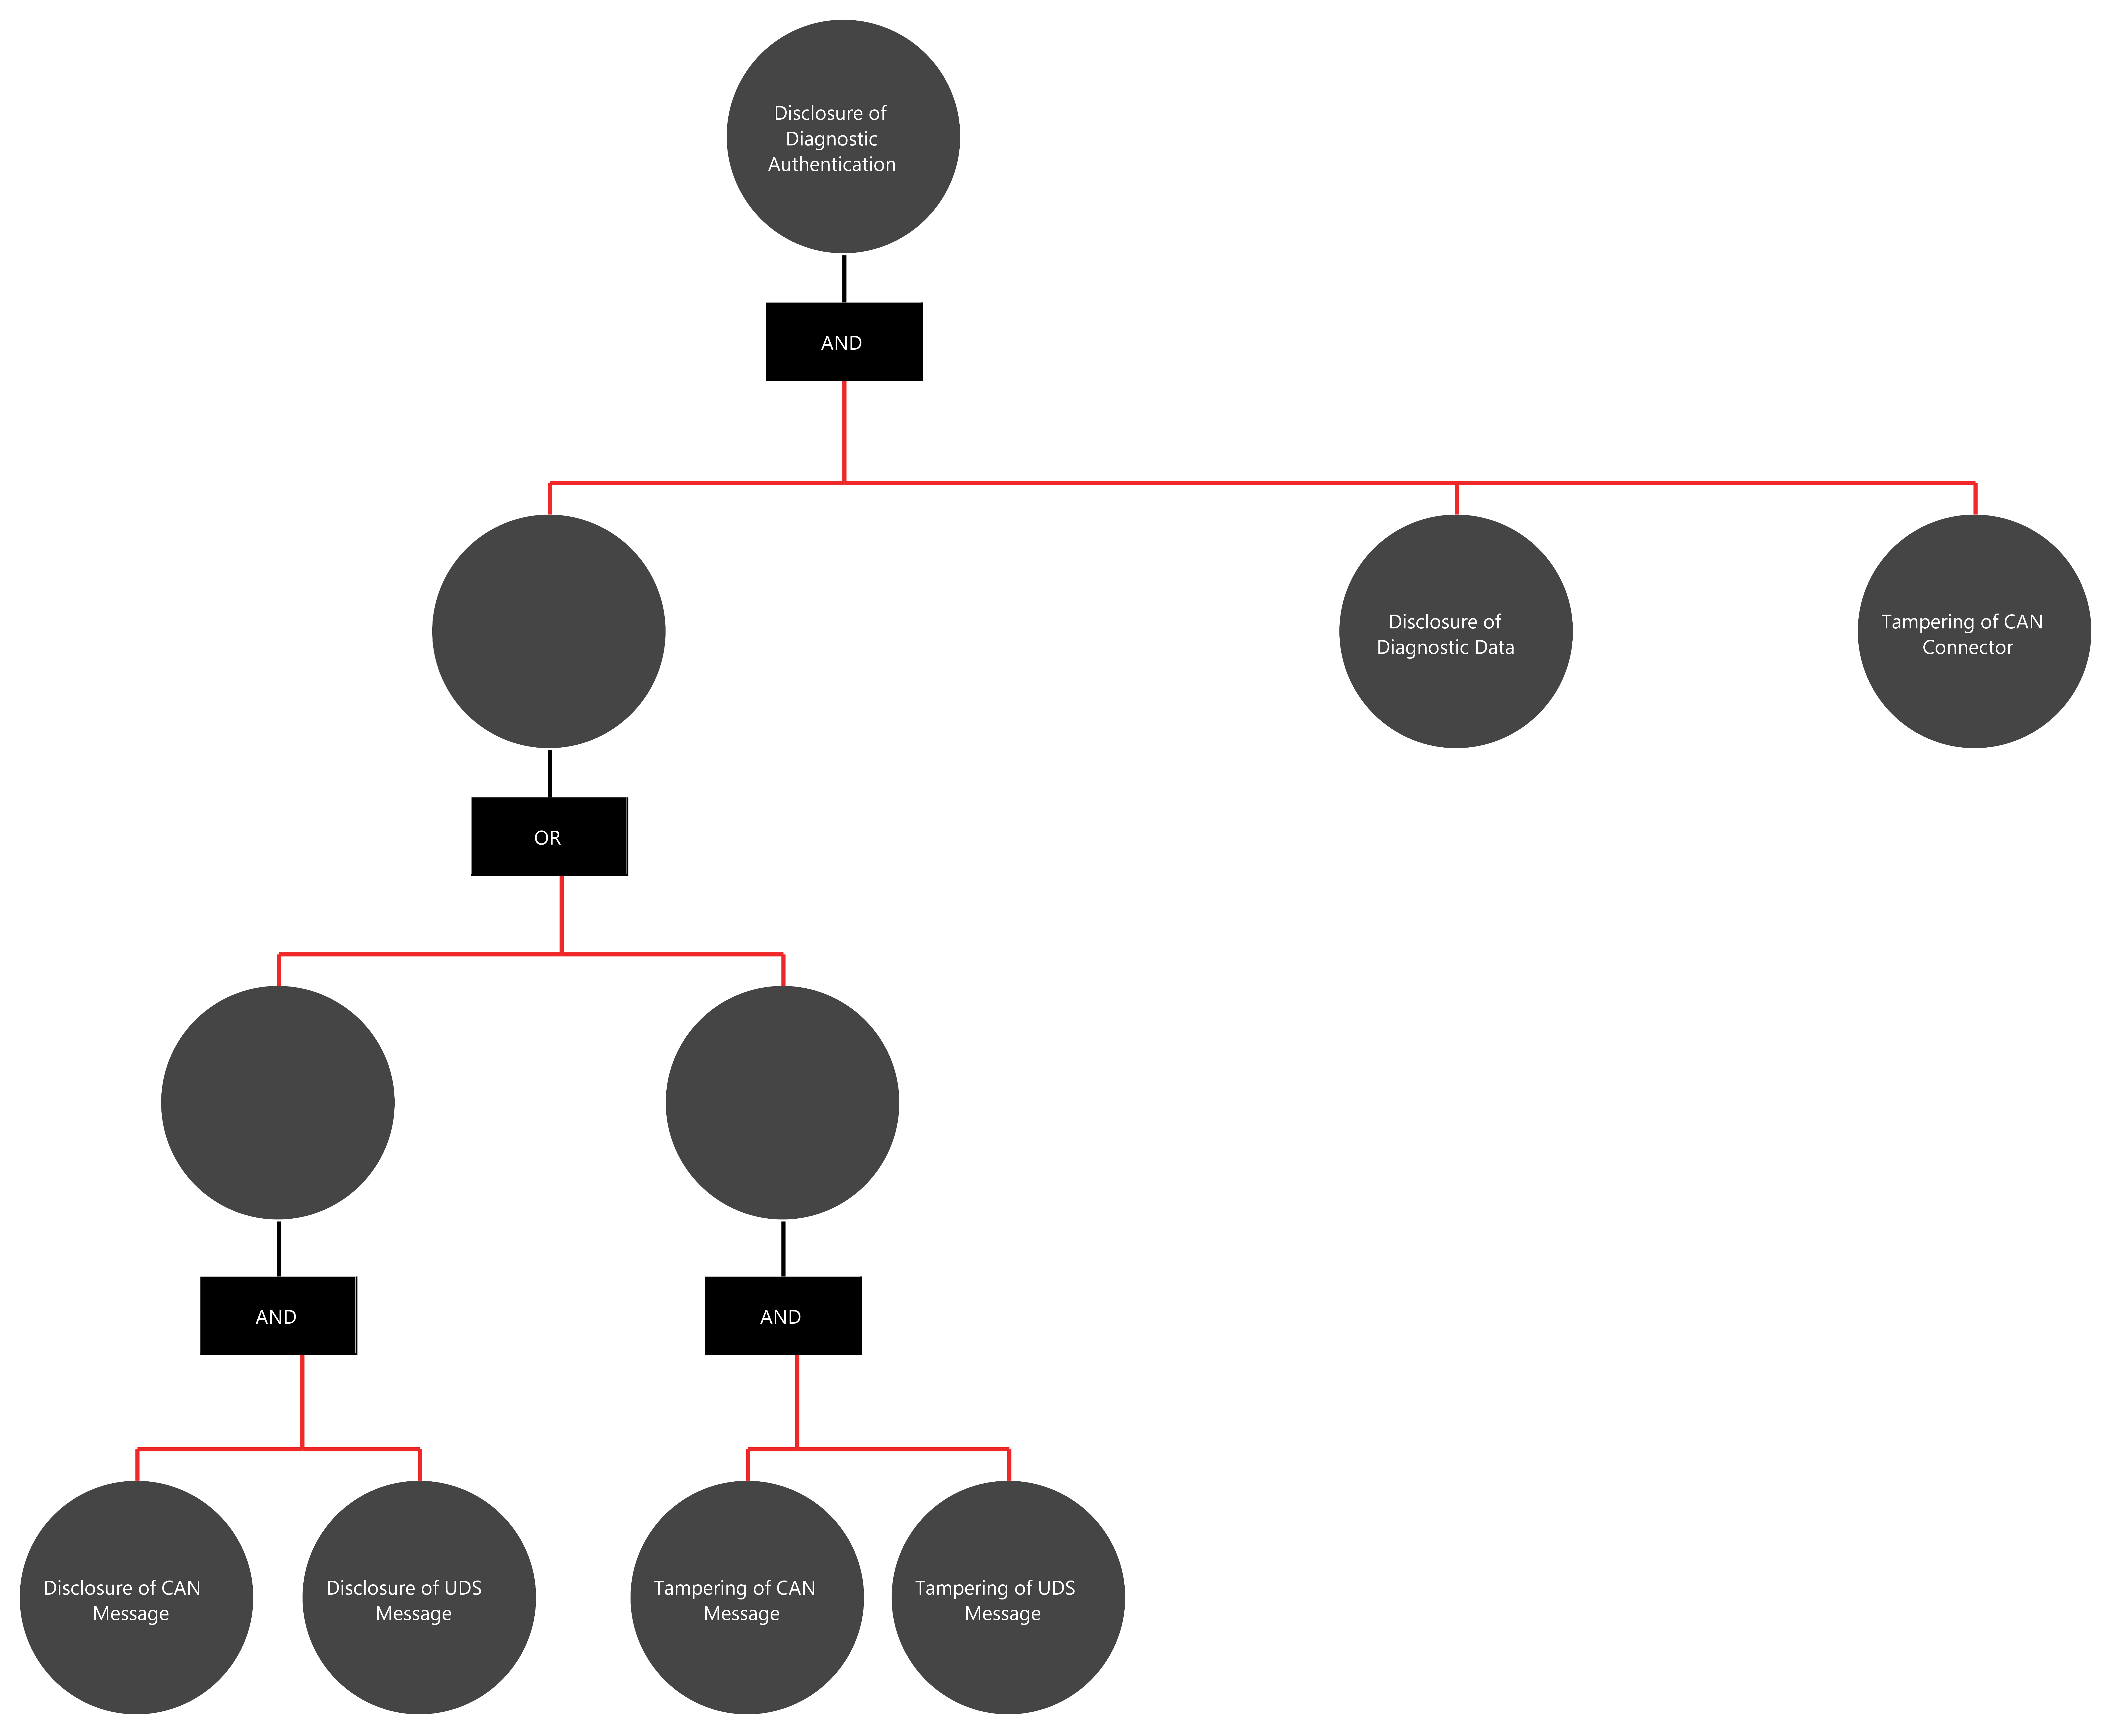
\includegraphics[width=120mm, keepaspectratio]{figures/AT-SECDIAG-00.png}
	\caption{Támadási fa a "Leak confidential data" károkozáshoz} 
	\label{fig:ff_leak_data}
\end{figure}

\newpage

Az \ref{fig:ff_access} ábrán, azt a támadási fát keressük amelyikkel a támadó hozzáférhet korlátozott elérésű diagnosztikai szolgáltatásokhoz. Hasonlóan a szoftver megváltoztatásához itt is szükségeltetik egy lehallgatási lépés, valamint ezen túl a megfelelő üzenetek konstruálása amely különböző mitigációk segítségével jól védhető.

\begin{figure}[!ht]
	\centering
	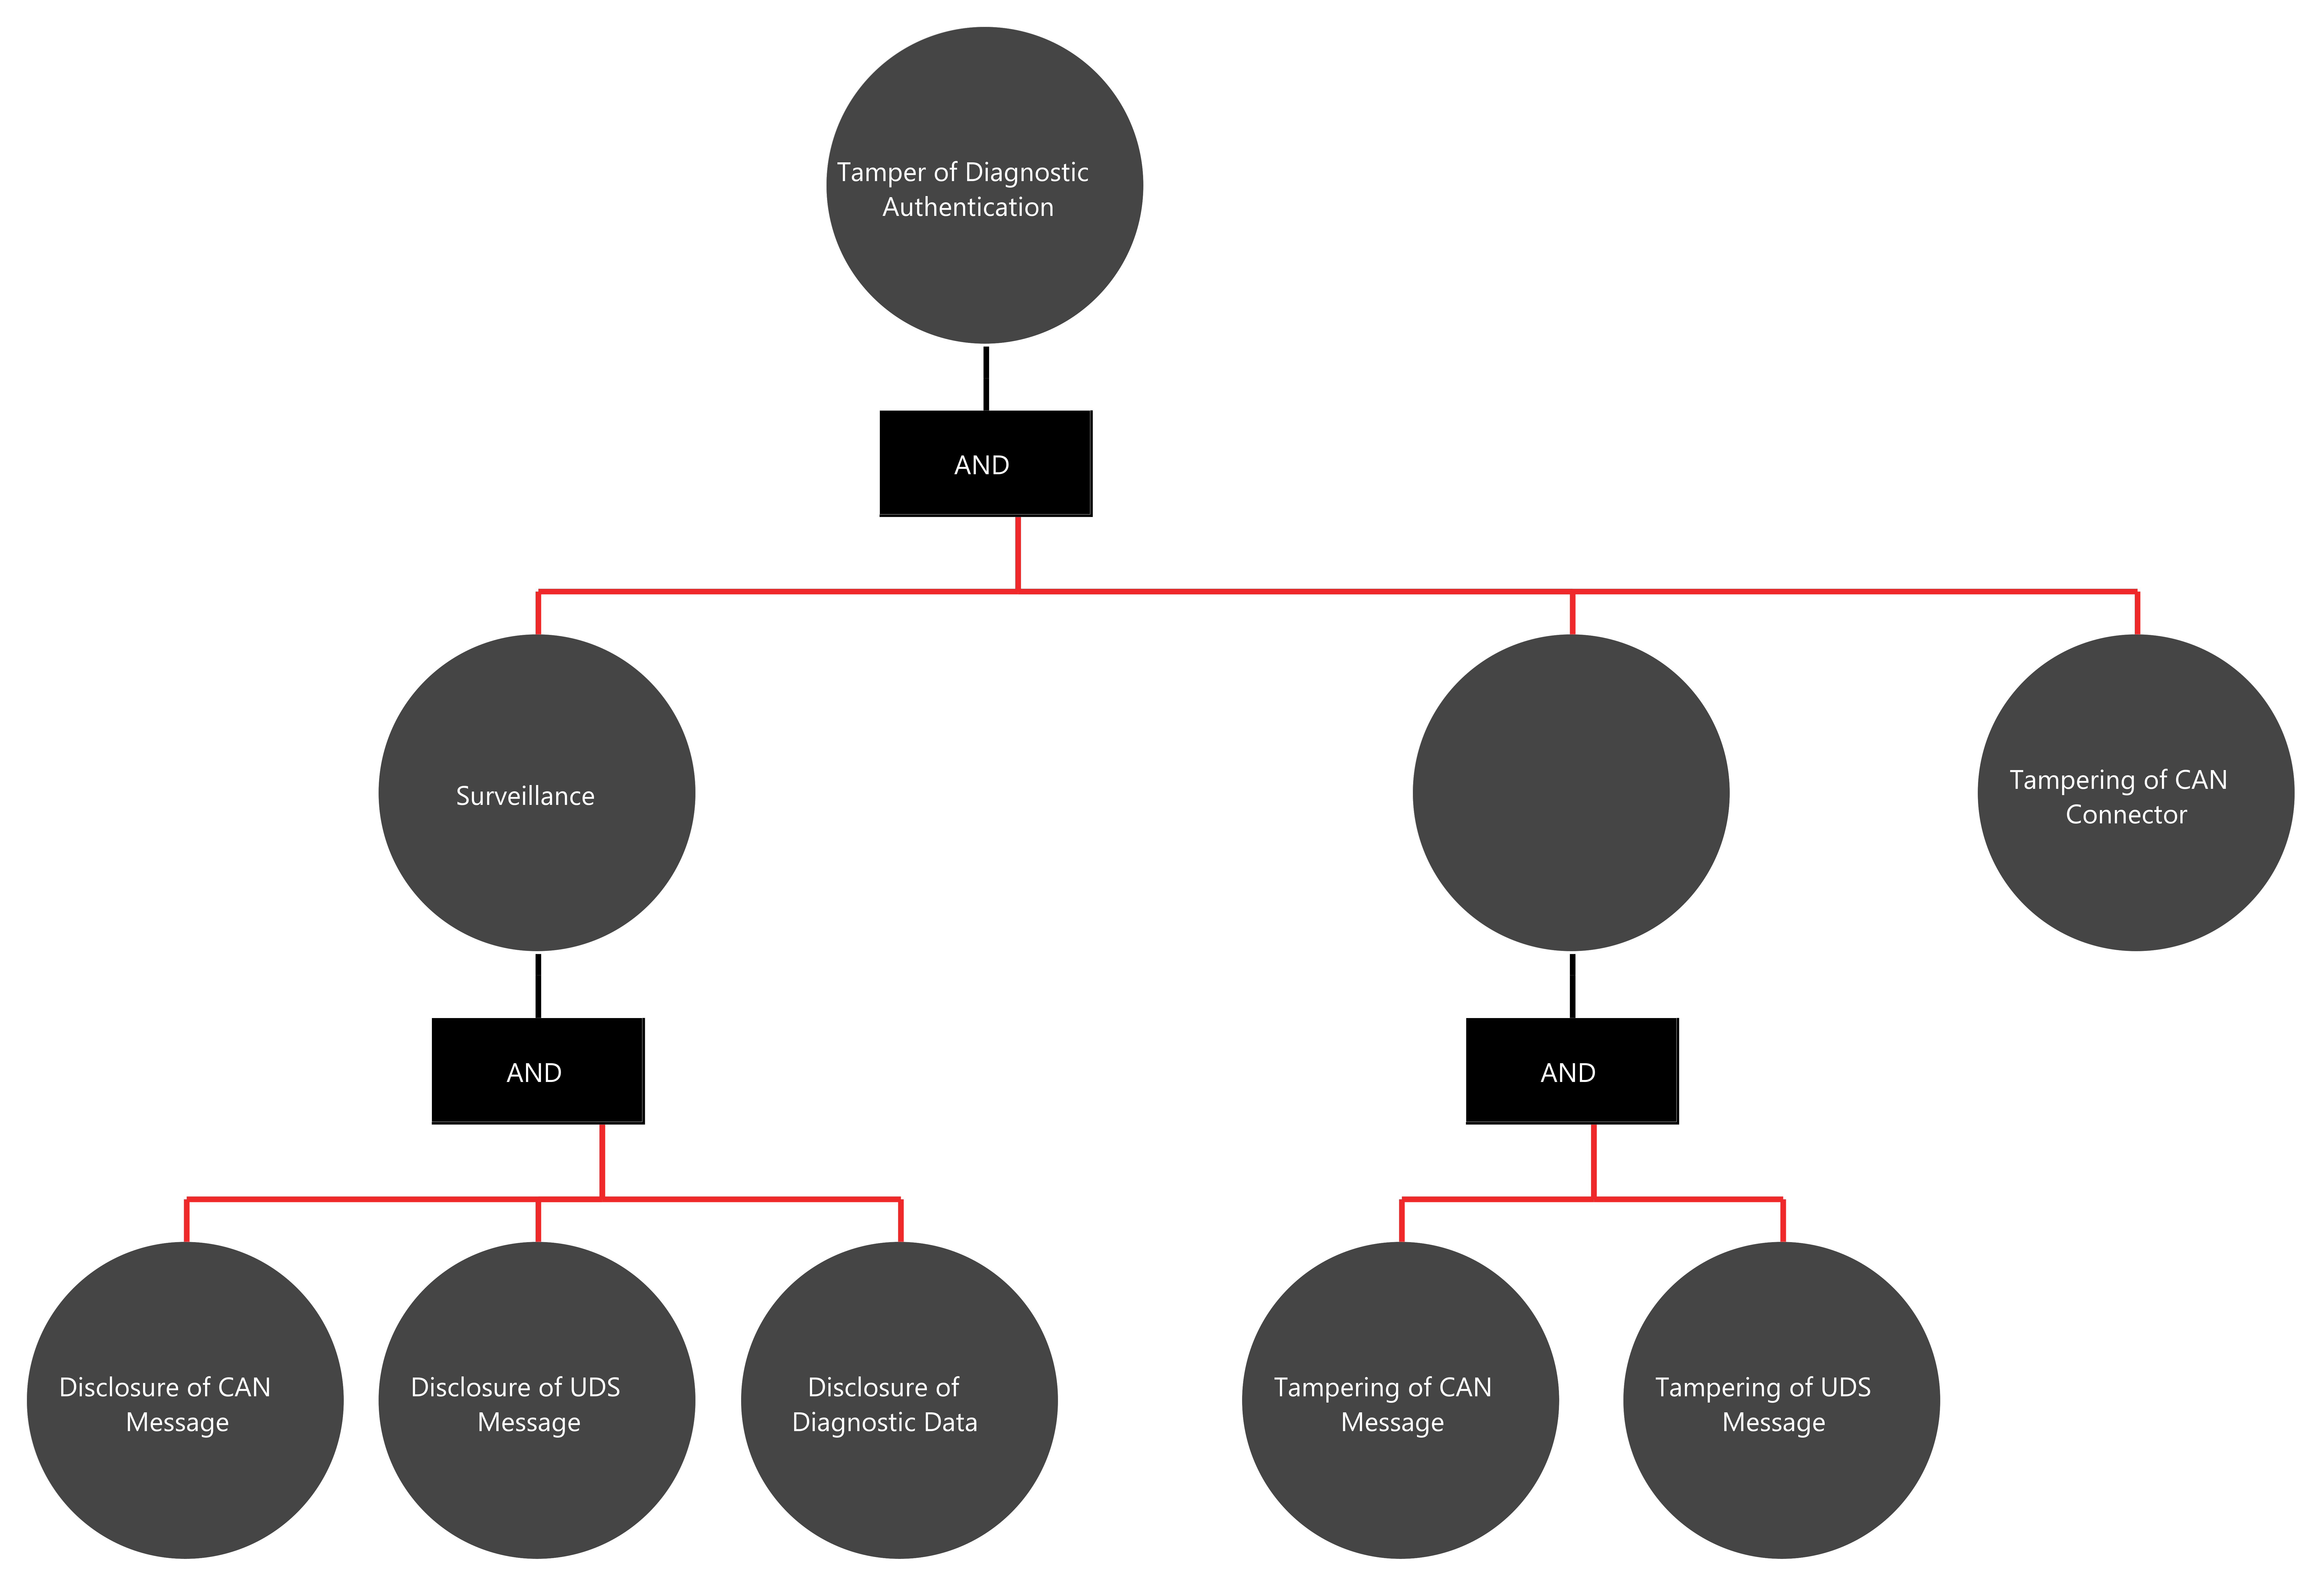
\includegraphics[width=120mm, keepaspectratio]{figures/AT-SECDIAG-01.png}
	\caption{Támadási fa a "Access unauthorized functionality" károkozáshoz} 
	\label{fig:ff_access}
\end{figure}

\newpage

Az \ref{fig:ff_block_auth} ábrán, az autentikációs lépések blokkolását okozó támadási fa látható. Ez is megegyezik a szoftver frissítés elérhetőségét sértő fához. Ennek az oka ezúttal is az, hogy a műveletet mivel mindkettő diagnosztikai szolgáltatás, ugyanazon lépésekkel kell megtenni ezen az absztrakciós szinten.

\begin{figure}[!ht]
	\centering
	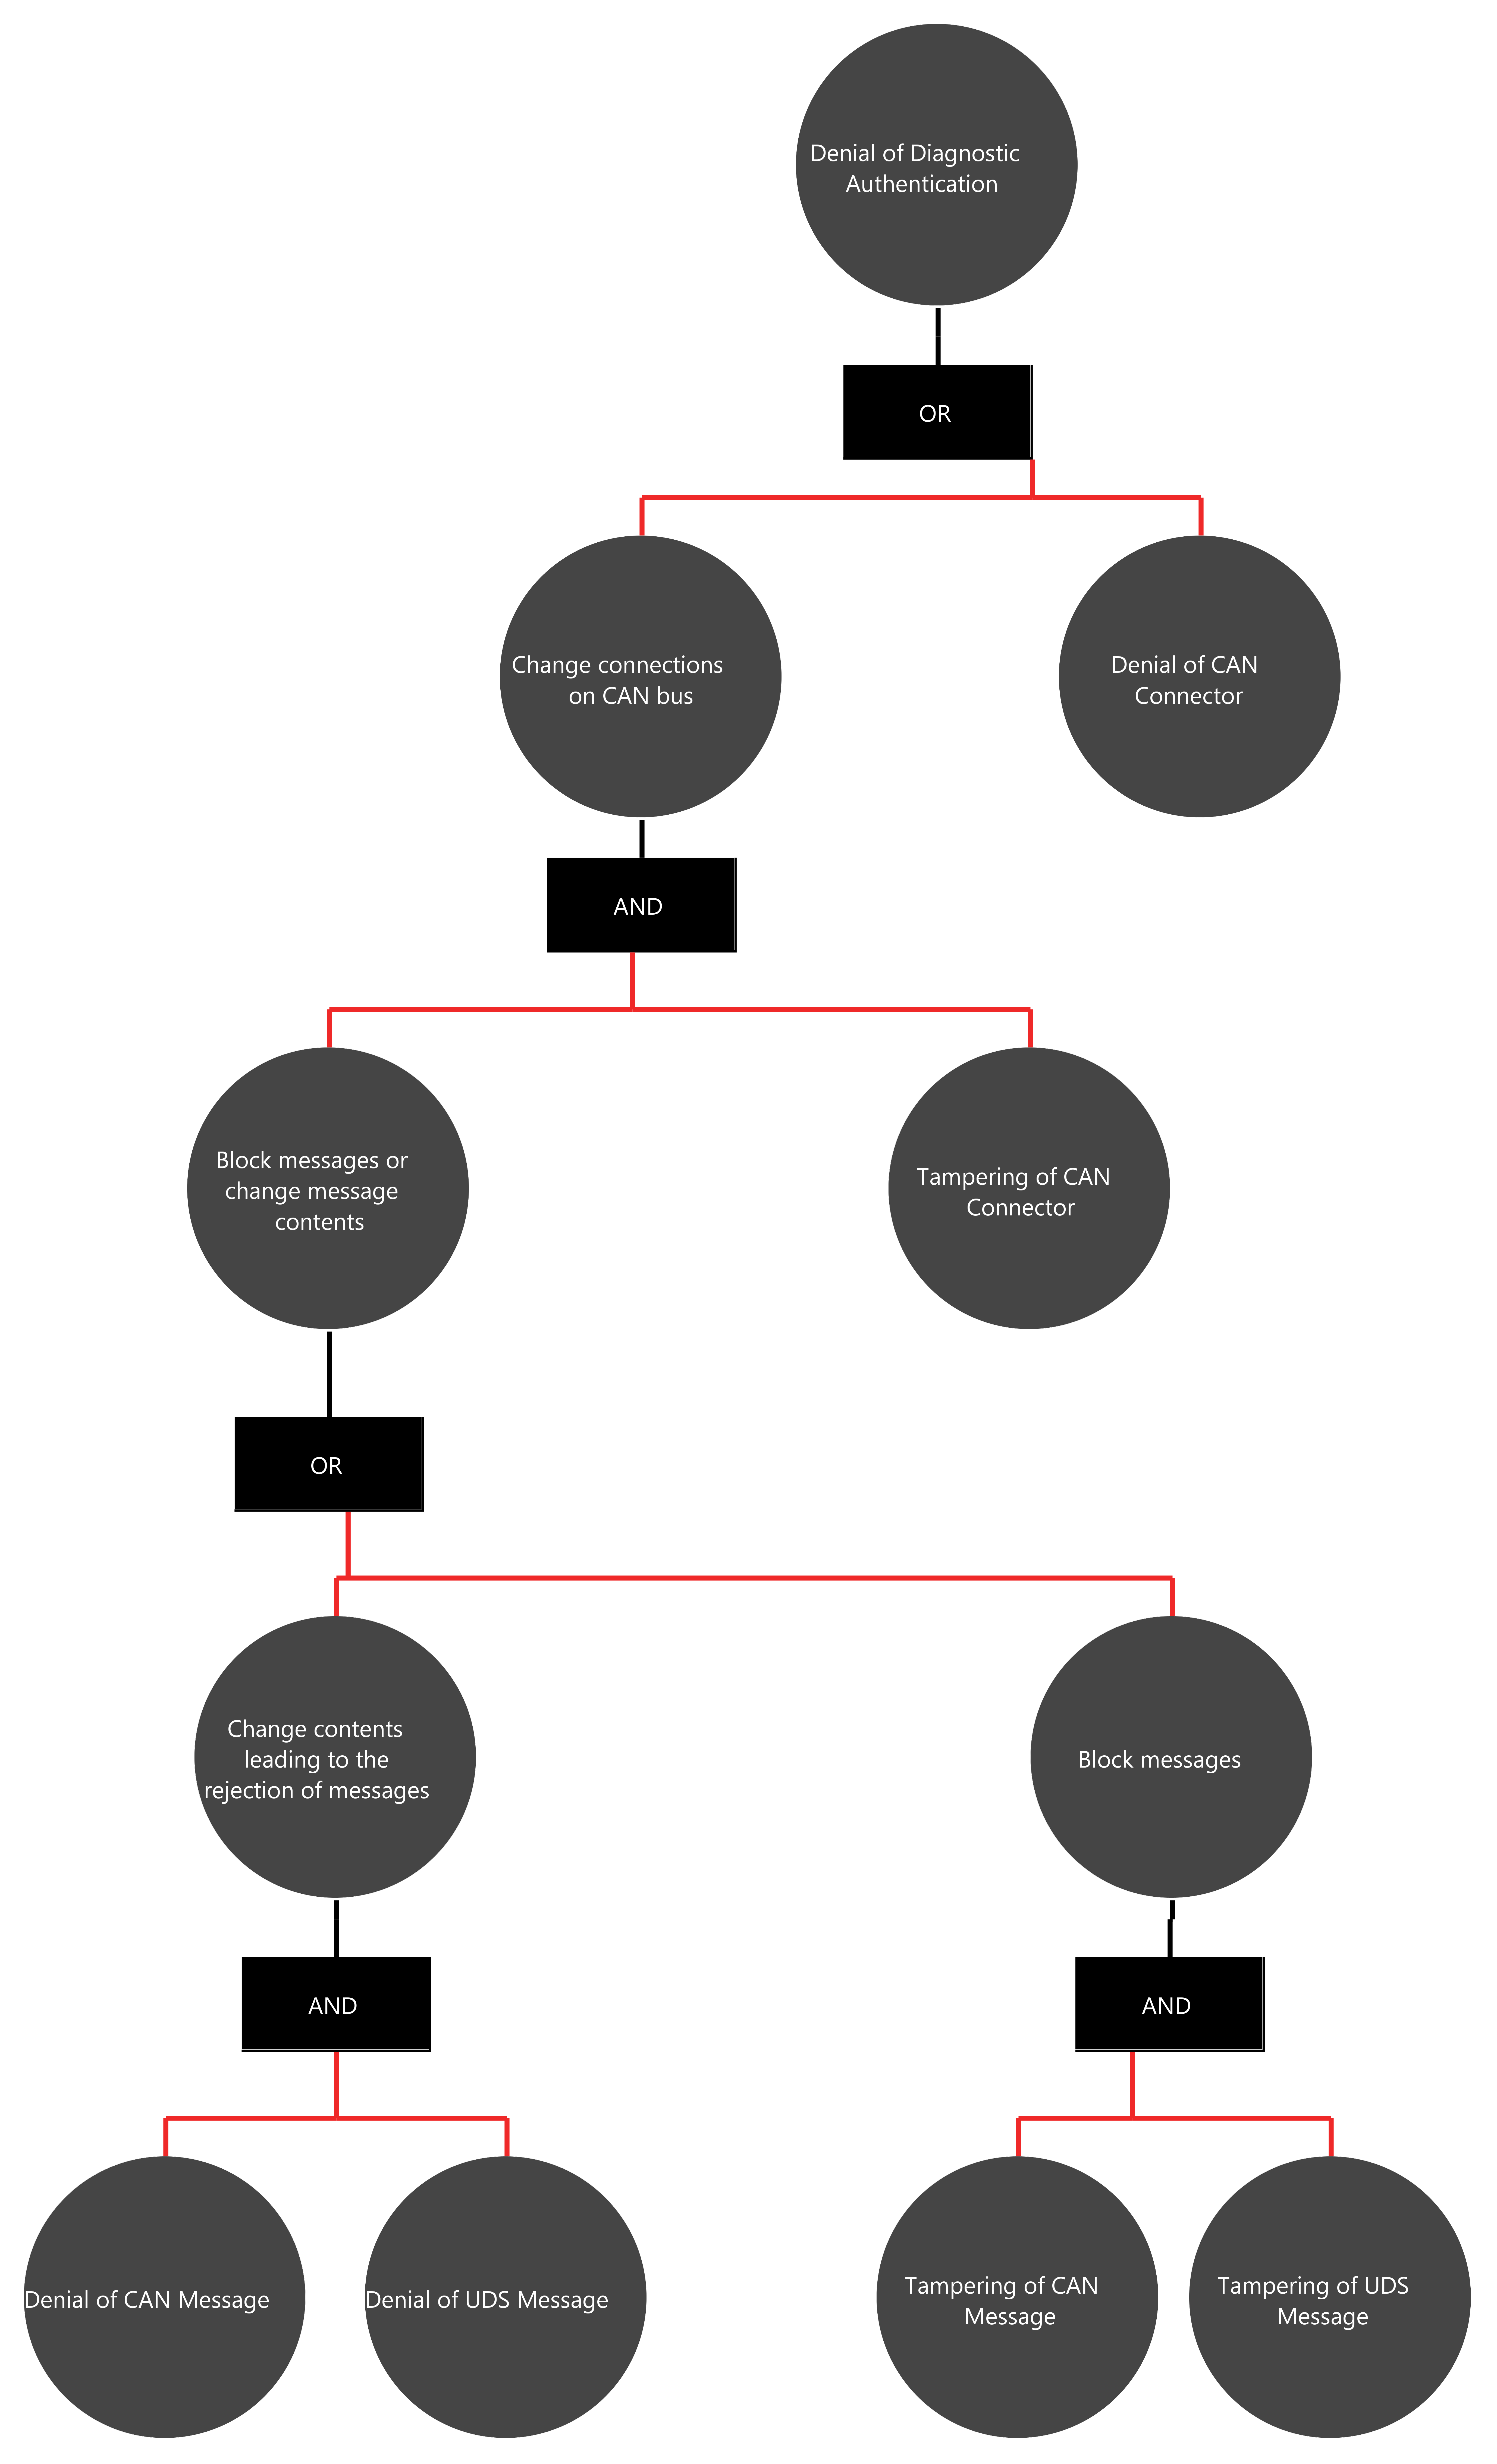
\includegraphics[width=120mm, keepaspectratio]{figures/AT-SECDIAG-02.png}
	\caption{Támadási fa a "Block authentication attempts" károkozáshoz} 
	\label{fig:ff_block_auth}
\end{figure}

Összességében elmondható, hogy a támadási fák konstruálása helyes, ezt bizonyítja az is, hogy a diagnosztikai rutinok támadási fái ugyanazon mintákat követik hiszen ugyan azon értékeket használja a két szolgáltatás. Amennyiben a szoftvert és a diagnosztikai adatot egy absztraktabb \textit{adat} meghatározással jelöltük volna a termékleírásban úgy elég lett volna kevesebb támadási fa azonban, ezeknek a külön vétele a manuális analízishez szükséges.

Szintén elmondható, hogy az eljárás gyors és ezáltal könnyen megismételhető. Ezen támadási fáknak a konstruálása ugyanazon atomi és legfelső eseményekből áll így a kontextus váltás a külön fák konstruálásakor jóval egyszerűbb.

Végül pedig a teljességet is teljesíti a támadási fa, minden termékleírásban valamint fenyegetésmodellben meghatározott érték elleni fenyegetés szerepel valamely támadási fában egyrészről, másrészről pedig megteremtettünk egy lekövethetőséget (traceability) a SW-, illetve HW-szintű fenyegetések valamint a károkozások között.

\section{Manuális analízis}

Az utolsó lépése az elemzésnek a manuális analízis. Itt először a hatásérték elemzést, utána pedig a támadás megvalósíthatóság elemzést végezzük el.\\

Ahogy az a \ref{fig:ff_imprate} ábrán látható a SFOP értékek mentén meg lettek határozva a hatásértékei az egyes károkozásoknak.

A legkomolyabb hatások a szoftver megváltoztatásával, törlésével, valamint a korlátozott hozzáférésű funkcionalitások használata lettek. Ezek értelemszerűen nagyobb kockázatot is jelentenek mint mondjuk az autentikációnak a blokkolása. Az elemzés az ISO 21434 \cite{ISO21434} által ajánlott és annak a függelékében lévő példa elemzések mintájára készültek el.\\

\begin{figure}[!ht]
	\centering
	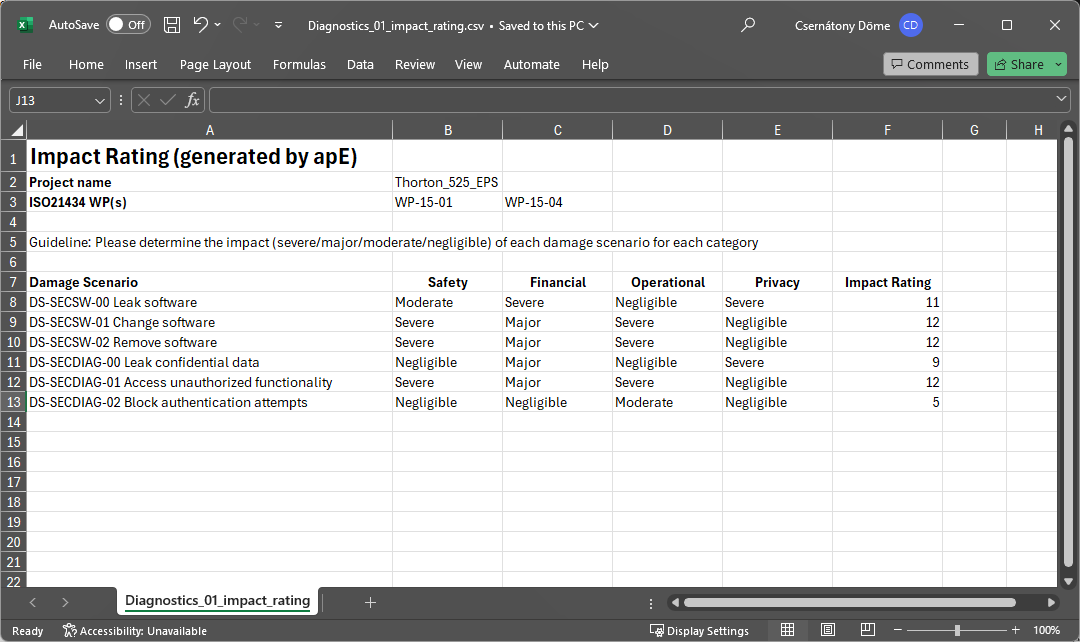
\includegraphics[width=120mm, keepaspectratio]{figures/ff_imprate.png}
	\caption{Hatásérték elemzés} 
	\label{fig:ff_imprate}
\end{figure}

Az \ref{fig:ff_attfeas} ábrán látható az értékelés az Attack Potential Based megközelítést használja, ez szintén az egyik ajánlása az ISO 21434 \cite{ISO21434} szabványnak, valamint szintén annak a függelékében lévő minta alapján készült el ez az elemzés is.

Ezen kiértékelések történhetnek egy szakértő által egyénileg, több stakeholder bevonásával illetve behatolástesztelő mérnökök támogatásával. A kiértékelés a támadó képességei és a rendelkezésre álló információk alapján ad egy becslést a támadási utak megvalósíthatóságára.

\begin{figure}[!ht]
	\centering
	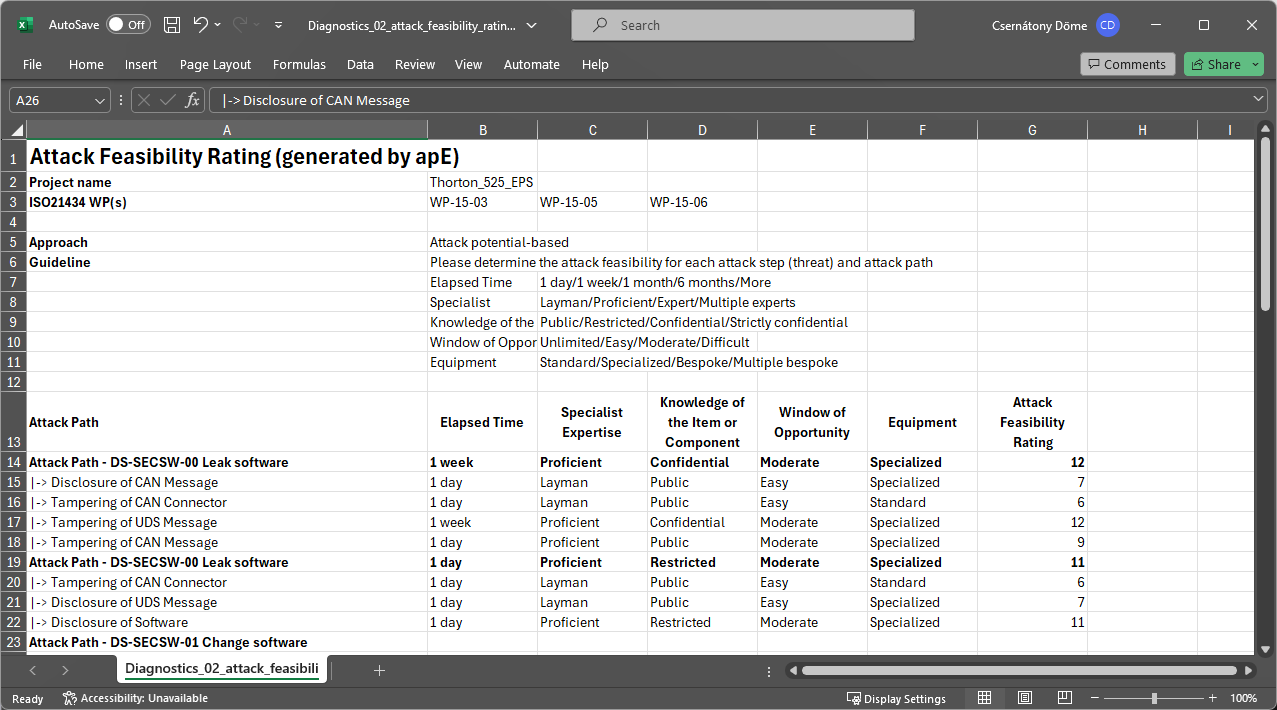
\includegraphics[width=120mm, keepaspectratio]{figures/ff_attfeas.png}
	\caption{Támadás megvalósíthatóság elemzés a "Leak software" károkozáshoz} 
	\label{fig:ff_attfeas}
\end{figure}

Ezzel befejezve a manuális analízisek eredményeinek a szabvány által leírt kombinációja alapján fog a kiberbiztonsági mérnök előállni a kockázati értékekkel amelyek mentén lehet eldönteni mely támadások azok amelyek valóban nagy kockázattal járnak és amelyekre védelmet kell biztosítani valamilyen formában.
\chapter{Összegzés}
%%----------------------------------------------------------------------------
\chapter{\LaTeX-eszközök}
\label{sec:LatexTools}
%----------------------------------------------------------------------------
\section{A szerkesztéshez használatos eszközök}
%----------------------------------------------------------------------------
Ez a sablon TeXstudio 2.8.8 szerkesztővel készült. A TeXstudio egy platformfüggetlen, Windows, Linux és Mac OS alatt is elérhető \LaTeX-szerkesztőprogram számtalan hasznos szolgáltatással (\refstruc{fig:TeXstudio}). A szoftver ingyenesen letölthető\footnote{A TeXstudio hivatalos oldala: \url{http://texstudio.sourceforge.net/}}.

\begin{figure}[!ht]
\centering
\includegraphics[width=150mm, keepaspectratio]{figures/TeXstudio.png}
\caption{A TeXstudio \LaTeX-szerkesztő.}
\label{fig:TeXstudio}
\end{figure}

A TeXstudio telepítése után érdemes még letölteni a magyar nyelvű helyesírásellenőrző-szótárakat hozzá. A TeXstudio az OpenOffice-hoz használatos formátumot tudja kezelni. A TeXstudio beállításainál a \verb+General+ fülön a \verb+Dictionaries+ résznél tudjuk megadni, hogy melyik szótárat használja.

Egy másik használható Windows alapú szerkesztőprogram a LEd\footnote{A LEd hivatalos oldala: \url{http://www.latexeditor.org/}} (LaTeX Editor), a TeXstudio azonban stabilabb, gyorsabb, és jobban használható.

%----------------------------------------------------------------------------
\section{A dokumentum lefordítása Windows alatt}
%----------------------------------------------------------------------------
A TeXstudio és a LEd kizárólag szerkesztőprogram (bár az utóbbiban DVI-nézegető is van), így a dokumentum fordításához szükséges eszközöket nem tartalmazza. Windows alatt alapvetően két lehetőség közül érdemes választani: MiKTeX (\url{http://miktex.org/}) és TeX Live (\url{http://www.tug.org/texlive/}) programcsomag. Az utóbbi működik Mac OS X, GNU/Linux alatt és Unix-származékokon is. A MiKTeX egy alapcsomag telepítése után mindig letölti a használt funkciókhoz szükséges, de lokálisan hiányzó \TeX-csomagokat, míg a TeX Live DVD ISO verzóban férhető hozzá. Ez a dokumentum TeX Live 2008 programcsomag segítségével fordult, amelynek DVD ISO verziója a megadott oldalról letölthető. A sablon lefordításához a disztribúcióban szereplő \verb+magyar.ldf+ fájlt a \verb+http://www.math.bme.hu/latex/+ változatra kell cserélni, vagy az utóbbi változatot be kell másolni a projekt-könyvtárba (ahogy ezt meg is tettük a sablonban) különben anomáliák tapasztalhatók a dokumentumban (pl. az ábra- és táblázat-aláírások formátuma nem a beállított lesz, vagy bizonyos oldalakon megjelenik alapértelmezésben egy fejléc). A TeX Live 2008-at még nem kell külön telepíteni a gépre, elegendő DVD-ről (vagy az ISO fájlból közvetlenül, pl. DaemonTools-szal) használni.

Ha a MiKTeX csomagot használjuk, akkor parancssorból a következő módon tudjuk újrafordítani a teljes dokumentumot:

\begin{lstlisting}[language=bash,frame=single,float=!ht]
$ texify -p thesis.tex
\end{lstlisting}

A \verb+texify+ parancs a MiKTex programcsomag \verb+miktex/bin+ alkönyvtárában található. A parancs gondoskodik arról, hogy a szükséges lépéseket (fordítás, hivatkozások generálása stb.) a megfelelő sorrendben elvégezze. A \verb+-p+ kapcsoló hatására PDF-et generál. A fordítást és az ideiglenes fájlok törlését elvégezhetjük a sablonhoz mellékelt \verb+manual_build.bat+ szkript segítségével is.

A \TeX-eszközöket tartalmazó programcsomag binárisainak elérési útját gyakran be kell állítani a szerkesztőprogramban, például TeXstudio esetén legegyszerűbben az \verb+Options / Configure TeXstudio... / Commands+ menüponttal előhívott dialógusablakban tehetjük ezt meg.

A PDF-\LaTeX~használata esetén a generált dokumentum közvetlenül PDF-formátumban áll rendelkezésre. Amennyiben a PDF-fájl egy PDF-nézőben (pl. Adobe Acrobat Reader vagy Foxit PDF Reader) meg van nyitva, akkor a fájlleírót a PDF-néző program tipikusan lefoglalja. Ilyen esetben a dokumentum újrafordítása hibaüzenettel kilép. Ha bezárjuk és újra megnyitjuk a PDF dokumentumot, akkor pedig a PDF-nézők többsége az első oldalon nyitja meg a dokumentumot, nem a legutóbb olvasott oldalon. Ezzel szemben például az egyszerű és ingyenes \textcolor{blue}{Sumatra PDF} nevű program képes arra, hogy a megnyitott dokumentum megváltozását detektálja, és frissítse a nézetet az aktuális oldal megtartásával.

%----------------------------------------------------------------------------
\section{Eszközök Linuxhoz}
%----------------------------------------------------------------------------
Linux operációs rendszer alatt is rengeteg szerkesztőprogram van, pl. a KDE alapú Kile jól használható. Ez ingyenesen letölthető, vagy éppenséggel az adott Linux-disztribúció eleve tartalmazza, ahogyan a dokumentum fordításához szükséges csomagokat is. Az Ubuntu Linux disztribúciók alatt például legtöbbször a \verb+texlive-*+ csomagok telepítésével használhatók a \LaTeX-eszközök. A jelen sablon fordításához szükséges csomagok (kb. 0,5 GB) az alábbi paranccsal telepíthetők:

\begin{lstlisting}[language=bash,morekeywords={sudo,apt\-get},alsoletter={-},breaklines=true]
$ sudo apt-get install texlive-latex-extra texlive-fonts-extra texlive-fonts-recommended texlive-lang-european texlive-xetex texlive-science
\end{lstlisting}

Amennyiben egy újabb csomag hozzáadása után hiányzó fájlra utaló hibát kapunk a fordítótól, telepítenünk kell az azt tartalmazó TeX Live csomagot. Ha pl. a \verb+bibentry+ csomagot szeretnénk használni, futtassuk az alábbi parancsot:

\begin{lstlisting}[language=bash,morekeywords={apt\-cache},alsoletter={-},breaklines=true]
$ apt-cache search bibentry
texlive-luatex - TeX Live: LuaTeX packages
\end{lstlisting}

Majd telepítsük fel a megfelelő TeX Live csomagot, jelen esetben a `texlive-lualatex`-et. (Egy LaTeX csomag több TeX Live csomagban is szerepelhet.)

Ha gyakran szerkesztünk más \LaTeX dokumentumokat is, kényelmes és biztos megoldás a teljes TeX Live disztribúció telepítése, ez azonban kb. 4 GB helyet igényel.

\begin{lstlisting}[language=bash,morekeywords={sudo,apt\-get},alsoletter={-},breaklines=true]
sudo apt-get install texlive-full
\end{lstlisting}

%%----------------------------------------------------------------------------
\chapter{A dolgozat formai kivitele}
%----------------------------------------------------------------------------
Az itt található információk egy része a BME VIK Hallgatói Képviselet által készített ,,Utolsó félév a villanykaron'' c. munkából lett kis változtatásokkal átemelve. Az eredeti dokumentum az alábbi linken érhető el: \url{http://vik.hk/hirek/diplomafelev-howto-2015}.

%----------------------------------------------------------------------------
\section{A dolgozat kimérete}
%----------------------------------------------------------------------------
Szakdolgozat esetében minimum 30, 45 körüli ajánlott oldalszám lehet az iránymutató. De mindenképp érdemes rákérdezni a konzulensnél is az elvárásokra, mert tanszékenként változóak lehetnek az elvárások.

Mesterképzésen a Diplomatervezés 1 esetében a beszámoló még inkább az Önálló laboratóriumi beszámolókhoz hasonlít, tanszékenként eltérő formai követelményekkel, -- egy legalább 30 oldal körüli dolgozat az elvárt -- és az elmúlt fél éves munkáról szól. De egyben célszerű, ha ez a végleges diplomaterv alapja is. (A végleges 60-90 oldal körülbelül a hasznos részre nézve)


%----------------------------------------------------------------------------
\section{A dolgozat nyelve}
%----------------------------------------------------------------------------
Mivel Magyarországon a hivatalos nyelv a magyar, ezért alapértelmezésben magyarul kell megírni a dolgozatot. Aki külföldi posztgraduális képzésben akar részt venni, nemzetközi szintű tudományos kutatást szeretne végezni, vagy multinacionális cégnél akar elhelyezkedni, annak célszerű angolul megírnia diplomadolgozatát. Mielőtt a hallgató az angol nyelvű verzió mellett dönt, erősen ajánlott mérlegelni, hogy ez mennyi többletmunkát fog a hallgatónak jelenteni fogalmazás és nyelvhelyesség terén, valamint -- nem utolsó sorban -- hogy ez mennyi többletmunkát fog jelenteni a konzulens illetve bíráló számára. Egy nehezen olvasható, netalán érthetetlen szöveg teher minden játékos számára.

%----------------------------------------------------------------------------
\section{A dokumentum nyomdatechnikai kivitele}
%----------------------------------------------------------------------------
A dolgozatot A4-es fehér lapra nyomtatva, 2,5 centiméteres margóval (+1~cm kötésbeni), 11--12 pontos betűmérettel, talpas betűtípussal és egyszeres sorközzel célszerű elkészíteni.
A másfeles sorköz (\verb+\onehalfspacing+ beállítás) is elfogadott szakdolgozatokban és diplomamunkákban, de ajánlott megtartani az egyszeres sorközt.

Annak érdekében, hogy a dolgozat külsőleg is igényes munka benyomását keltse, érdemes figyelni az alapvető tipográfiai szabályok betartására~\cite{Jeney}.

%% !TeX spellcheck = hu_HU
% !TeX encoding = UTF-8
% !TeX program = xelatex
%----------------------------------------------------------------------------
\chapter{A \LaTeX-sablon használata}
%----------------------------------------------------------------------------

Ebben a fejezetben röviden, implicit módon bemutatjuk a sablon használatának módját, ami azt jelenti, hogy sablon használata ennek a dokumentumnak a forráskódját tanulmányozva válik teljesen világossá. Amennyiben a szoftver-keretrendszer telepítve van, a sablon alkalmazása és a dolgozat szerkesztése \LaTeX-ben a sablon segítségével tapasztalataink szerint jóval hatékonyabb, mint egy WYSWYG (\emph{What You See is What You Get}) típusú szövegszerkesztő esetén (pl. Microsoft Word, OpenOffice).

%----------------------------------------------------------------------------
\section{Címkék és hivatkozások}
%----------------------------------------------------------------------------
A \LaTeX~dokumentumban címkéket (\verb+\label+) rendelhetünk ábrákhoz, táblázatokhoz, fejezetekhez, listákhoz, képletekhez stb. Ezekre a dokumentum bármely részében hivatkozhatunk, a hivatkozások automatikusan feloldásra kerülnek.

A sablonban makrókat definiáltunk a hivatkozások megkönnyítéséhez. Ennek megfelelően minden ábra (\emph{figure}) címkéje \verb+fig:+ kulcsszóval kezdődik, míg minden táblázat (\emph{table}), képlet (\emph{equation}), fejezet (\emph{section}) és lista (\emph{listing}) rendre a \verb+tab:+, \verb+eq:+, \verb+sec:+ és \verb+lst:+ kulcsszóval kezdődik, és a kulcsszavak után tetszőlegesen választott címke használható. Ha ezt a konvenciót betartjuk, akkor az előbbi objektumok számára rendre a \verb+\figref+, \verb+\tabref+, \verb+\eqref+, \verb+\sectref+ és \verb+\listref+ makrókkal hivatkozhatunk. A makrók paramétere a címke, amelyre hivatkozunk (a kulcsszó nélkül). Az összes említett hivatkozástípus, beleértve az \verb+\url+ kulcsszóval bevezetett web-hivatkozásokat is a  \verb+hyperref+\footnote{Segítségével a dokumentumban megjelenő hivatkozások nem csak dinamikussá válnak, de színezhetők is, bővebbet erről a csomag dokumentációjában találunk. Ez egyúttal egy példa lábjegyzet írására.} csomagnak köszönhetően aktívak a legtöbb PDF-nézegetőben, rájuk kattintva a dokumentum megfelelő oldalára ugrik a PDF-néző vagy a megfelelő linket megnyitja az alapértelmezett böngészővel. A \verb+hyperref+ csomag a kimeneti PDF-dokumentumba könyvjelzőket is készít a tartalomjegyzékből. Ez egy szintén aktív tartalomjegyzék, amelynek elemeire kattintva a nézegető behozza a kiválasztott fejezetet.

%----------------------------------------------------------------------------
\section{Ábrák és táblázatok}
%----------------------------------------------------------------------------
Használjunk vektorgrafikus ábrákat, ha van rá módunk. PDFLaTeX használata esetén PDF formátumú ábrákat lehet beilleszteni könnyen, az EPS (PostScript) vektorgrafikus képformátum beillesztését a PDFLaTeX közvetlenül nem támogatja (de lehet konvertálni, lásd később). Ha vektorgrafikus formában nem áll rendelkezésünkre az ábra, akkor a  veszteségmentes PNG, valamint a veszteséges JPEG formátumban érdemes elmenteni.  Figyeljünk arra, hogy ilyenkor a képek felbontása elég nagy legyen ahhoz, hogy nyomtatásban is megfelelő minőséget nyújtson (legalább 300 dpi javasolt). A dokumentumban felhasznált képfájlokat a dokumentum forrása mellett érdemes tartani, archiválni, mivel ezek hiányában a dokumentum nem fordul újra. Ha lehet, a vektorgrafikus képeket vektorgrafikus formátumban is érdemes elmenteni az újrafelhasználhatóság (az átszerkeszthetőség) érdekében.

Kapcsolási rajzok legtöbbször kimásolhatók egy vektorgrafikus programba (pl. CorelDraw) és onnan nagyobb felbontással raszterizálva kimenthatők PNG formátumban. Ugyanakkor kiváló ábrák készíthetők Microsoft Visio vagy hasonló program használatával is: Visio-ból az ábrák közvetlenül PDF-be is menthetők.

Lehetőségeink Matlab ábrák esetén:
\begin{itemize}
	\item Képernyőlopás (\emph{screenshot}) is elfogadható minőségű lehet a dokumentumban, de általában jobb felbontást is el lehet érni más módszerrel.
	\item A Matlab ábrát a \verb+File/Save As+ opcióval lementhetjük PNG formátumban (ugyanaz itt is érvényes, mint korábban, ezért nem javasoljuk).
	\item A Matlab ábrát az \verb+Edit/Copy figure+ opcióval kimásolhatjuk egy vektorgrafikus programba is és onnan nagyobb felbontással raszterizálva kimenthatjük PNG formátumban (nem javasolt).
	\item Javasolt megoldás: az ábrát a \verb+File/Save As+ opcióval EPS \emph{vektorgrafikus} formátumban elmentjük, PDF-be konvertálva beillesztjük a dolgozatba.
\end{itemize}
Az EPS kép az \verb+epstopdf+ programmal\footnote{a korábban említett \LaTeX-disztribúciókban megtalálható} konvertálható PDF formátumba. Célszerű egy batch-fájlt készíteni az összes EPS ábra lefordítására az alábbi módon (ez Windows alatt működik).
\begin{lstlisting}[language=]
@echo off
for %%j in (*.eps) do (
  echo converting file "%%j"
  epstopdf "%%j"
)
echo done .
\end{lstlisting}

Egy ilyen parancsfájlt (\verb+convert.cmd+) elhelyeztük a sablon \verb+figures\eps+ könyvtárába, így a felhasználónak csak annyi a dolga, hogy a \verb+figures\eps+ könyvtárba kimenti az EPS formátumú vektorgrafikus képet, majd lefuttatja a \verb+convert.cmd+ parancsfájlt, ami PDF-be konvertálja az EPS fájlt.

Ezek után a PDF-ábrát ugyanúgy lehet a dokumentumba beilleszteni, mint a PNG-t vagy a JPEG-et. A megoldás előnye, hogy a lefordított dokumentumban is vektorgrafikusan tárolódik az ábra, így a mérete jóval kisebb, mintha raszterizáltuk volna beillesztés előtt. Ez a módszer minden -- az EPS formátumot ismerő -- vektorgrafikus program (pl. CorelDraw) esetén is használható.

A képek beillesztésére \az+\refstruc{sec:LatexTools}ben mutattunk be példát (\refstruc{fig:TeXstudio}). Az előző mondatban egyúttal az automatikusan feloldódó ábrahivatkozásra is láthatunk példát. Több képfájlt is beilleszthetünk egyetlen ábrába. Az egyes képek közötti horizontális és vertikális margót metrikusan szabályozhatjuk (\refstruc{fig:HVSpaces}). Az ábrák elhelyezését számtalan tipográfiai szabály egyidejű teljesítésével a fordító maga végzi, a dokumentum írója csak preferenciáit jelezheti a fordító felé (olykor ez bosszúságot is okozhat, ilyenkor pl. a kép méretével lehet játszani).

\begin{figure}[!ht]
	\centering
	\includegraphics[width=67mm, keepaspectratio]{figures/TeXstudio.png}\hspace{1cm}
	\includegraphics[width=67mm, keepaspectratio]{figures/TeXstudio.png}\\\vspace{5mm}
	\includegraphics[width=67mm, keepaspectratio]{figures/TeXstudio.png}\hspace{1cm}
	\includegraphics[width=67mm, keepaspectratio]{figures/TeXstudio.png}
	\caption{Több képfájl beillesztése esetén térközöket is érdemes használni.}
	\label{fig:HVSpaces}
\end{figure}

A táblázatok használatára \aref{tab:TabularExample}~táblázat mutat példát. A táblázatok formázásához hasznos tanácsokat találunk a \verb+booktabs+ csomag dokumentációjában.

\begin{table}[ht]
	\footnotesize
	\centering
	\begin{tabular}{ l c c }
		\toprule
		Órajel & Frekvencia & Cél pin \\
		\midrule
		CLKA & 100 MHz & FPGA CLK0\\
		CLKB & 48 MHz  & FPGA CLK1\\
		CLKC & 20 MHz  & Processzor\\
		CLKD & 25 MHz  & Ethernet chip \\
		CLKE & 72 MHz  & FPGA CLK2\\
		XBUF & 20 MHz  & FPGA CLK3\\
		\bottomrule
	\end{tabular}
	\caption{Az órajel-generátor chip órajel-kimenetei.}
	\label{tab:TabularExample}
\end{table}


%----------------------------------------------------------------------------
\section{Felsorolások és listák}
%----------------------------------------------------------------------------
Számozatlan felsorolásra mutat példát a jelenlegi bekezdés:
\begin{itemize}
	\item \emph{első bajusz:} ide lehetne írni az első elem kifejését,
	\item \emph{második bajusz:} ide lehetne írni a második elem kifejését,
	\item \emph{ez meg egy szakáll:} ide lehetne írni a harmadik elem kifejését.
\end{itemize}

Számozott felsorolást is készíthetünk az alábbi módon:
\begin{enumerate}
	\item \emph{első bajusz:} ide lehetne írni az első elem kifejését, és ez a kifejtés így néz ki, ha több sorosra sikeredik,
	\item \emph{második bajusz:} ide lehetne írni a második elem kifejését,
	\item \emph{ez meg egy szakáll:} ide lehetne írni a harmadik elem kifejését.
\end{enumerate}
A felsorolásokban sorok végén vessző, az utolsó sor végén pedig pont a szokásos írásjel. Ez alól kivételt képezhet, ha az egyes elemek több teljes mondatot tartalmaznak.

Listákban a dolgozat szövegétől elkülönítendő kódrészleteket, programsorokat, pszeudo-kódokat jeleníthetünk meg (\ref{lst:Example}.~kódrészlet).
\begin{lstlisting}[language=tex,caption=A fenti számozott felsorolás \LaTeX-forráskódja,label=lst:Example]
\begin{enumerate}
	\item \emph{els(*@ő@*) bajusz:} ide lehetne írni az els(*@ő@*) elem kifejését,
	és ez a kifejtés így néz ki, ha több sorosra sikeredik,
	\item \emph{második bajusz:} ide lehetne írni a második elem kifejését,
	\item \emph{ez meg egy szakáll:} ide lehetne írni a harmadik elem kifejését.
\end{enumerate}
\end{lstlisting}
A lista keretét, háttérszínét, egész stílusát megválaszthatjuk. Ráadásul különféle programnyelveket és a nyelveken belül kulcsszavakat is definiálhatunk, ha szükséges. Erről bővebbet a \verb+listings+ csomag hivatalos leírásában találhatunk.

%----------------------------------------------------------------------------
\section{Képletek}
%----------------------------------------------------------------------------
Ha egy formula nem túlságosan hosszú, és nem akarjuk hivatkozni a szövegből, mint például a $e^{i\pi}+1=0$ képlet, \emph{szövegközi képletként} szokás leírni. Csak, hogy másik példát is lássunk, az $U_i=-d\Phi/dt$ Faraday-törvény a $\rot E=-\frac{dB}{dt}$ differenciális alakban adott Maxwell-egyenlet felületre vett integráljából vezethető le. Látható, hogy a \LaTeX-fordító a sorközöket betartja, így a szöveg szedése esztétikus marad szövegközi képletek használata esetén is.

Képletek esetén az általános konvenció, hogy a kisbetűk skalárt, a kis félkövér betűk ($\mathbf{v}$) oszlopvektort -- és ennek megfelelően $\mathbf{v}^T$ sorvektort -- a kapitális félkövér betűk ($\mathbf{V}$) mátrixot jelölnek. Ha ettől el szeretnénk térni, akkor az alkalmazni kívánt jelölésmódot célszerű külön alfejezetben definiálni. Ennek megfelelően, amennyiben $\mathbf{y}$ jelöli a mérések vektorát, $\mathbf{\vartheta}$ a paraméterek vektorát és $\hat{\mathbf{y}}=\mathbf{X}\vartheta$ a paraméterekben lineáris modellt, akkor a \emph{Least-Squares} értelemben optimális paraméterbecslő $\hat{\mathbf{\vartheta}}_{LS}=(\mathbf{X}^T\mathbf{X})^{-1}\mathbf{X}^T\mathbf{y}$ lesz.

Emellett kiemelt, sorszámozott képleteket is megadhatunk, ennél az \verb+equation+ és a \verb+eqnarray+ környezetek helyett a korszerűbb \verb+align+ környezet alkalmazását javasoljuk (több okból, különféle problémák elkerülése végett, amelyekre most nem térünk ki). Tehát
\begin{align}
\dot{\mathbf{x}}&=\mathbf{A}\mathbf{x}+\mathbf{B}\mathbf{u},\\
\mathbf{y}&=\mathbf{C}\mathbf{x},
\end{align}
ahol $\mathbf{x}$ az állapotvektor, $\mathbf{y}$ a mérések vektora és $\mathbf{A}$, $\mathbf{B}$ és $\mathbf{C}$ a rendszert leíró paramétermátrixok. Figyeljük meg, hogy a két egyenletben az egyenlőségjelek egymáshoz igazítva jelennek meg, mivel a mindkettőt az \& karakter előzi meg a kódban. Lehetőség van számozatlan kiemelt képlet használatára is, például
\begin{align}
\dot{\mathbf{x}}&=\mathbf{A}\mathbf{x}+\mathbf{B}\mathbf{u},\nonumber\\
\mathbf{y}&=\mathbf{C}\mathbf{x}\nonumber.
\end{align}
Mátrixok felírására az $\mathbf{A}\mathbf{x}=\mathbf{b}$ inhomogén lineáris egyenlet részletes kifejtésével mutatunk példát:
\begin{align}
\begin{bmatrix}
a_{11} & a_{12} & \dots & a_{1n}\\
a_{21} & a_{22} & \dots & a_{2n}\\
\vdots & \vdots & \ddots & \vdots\\
a_{m1} & a_{m2} & \dots & a_{mn}
\end{bmatrix}
\begin{pmatrix}x_1\\x_2\\\vdots\\x_n\end{pmatrix}=
\begin{pmatrix}b_1\\b_2\\\vdots\\b_m\end{pmatrix}.
\end{align}
A \verb+\frac+ utasítás hatékonyságát egy általános másodfokú tag átviteli függvényén keresztül mutatjuk be, azaz
\begin{align}
W(s)=\frac{A}{1+2T\xi s+s^2T^2}.
\end{align}
A matematikai mód minden szimbólumának és képességének a bemutatására természetesen itt nincs lehetőség, de gyors referenciaként hatékonyan használhatók a következő linkek:\\
\indent\url{http://www.artofproblemsolving.com/LaTeX/AoPS_L_GuideSym.php},\\
\indent\url{http://www.ctan.org/tex-archive/info/symbols/comprehensive/symbols-a4.pdf},\\
\indent\url{ftp://ftp.ams.org/pub/tex/doc/amsmath/short-math-guide.pdf}.\\
Ez pedig itt egy magyarázat, hogy miért érdemes \verb+align+ környezetet használni:\\
\indent\url{http://texblog.net/latex-archive/maths/eqnarray-align-environment/}.

%----------------------------------------------------------------------------
\section{Irodalmi hivatkozások}
\label{sec:HowtoReference}
%----------------------------------------------------------------------------
Egy \LaTeX~dokumentumban az irodalmi hivatkozások definíciójának két módja van. Az egyik a \verb+\thebibliograhy+ környezet használata a dokumentum végén, az \verb+\end{document}+ lezárás előtt.
\begin{lstlisting}[language=tex]
\begin{thebibliography}{9}

\bibitem{Lamport94} Leslie Lamport, \emph{\LaTeX: A Document Preparation System}.
Addison Wesley, Massachusetts, 2nd Edition, 1994.

\end{thebibliography}
\end{lstlisting}

Ezek után a dokumentumban a \verb+\cite{Lamport94}+ utasítással hivatkozhatunk a forrásra. A fenti megadás viszonylag kötetlen, a szerző maga formázza az irodalomjegyzéket (ami gyakran inkonzisztens eredményhez vezet).

Egy sokkal professzionálisabb módszer a BiB\TeX{} használata, ezért ez a sablon is ezt támogatja. Ebben az esetben egy külön szöveges adatbázisban definiáljuk a forrásmunkákat, és egy külön stílusfájl határozza meg az irodalomjegyzék kinézetét. Ez, összhangban azzal, hogy külön formátumkonvenció határozza meg a folyóirat-, a könyv-, a konferenciacikk- stb. hivatkozások kinézetét az irodalomjegyzékben (a sablon használata esetén ezzel nem is kell foglalkoznia a hallgatónak, de az eredményt célszerű ellenőrizni). felhasznált hivatkozások adatbázisa egy \verb+.bib+ kiterjesztésű szöveges fájl, amelynek szerkezetét a \Aref{lst:Bibtex} kódrészlet demonstrálja. A forrásmunkák bevitelekor a sor végi vesszők külön figyelmet igényelnek, mert hiányuk a BiB\TeX-fordító hibaüzenetét eredményezi. A forrásmunkákat típus szerinti kulcsszó vezeti be (\verb+@book+ könyv, \verb+@inproceedings+ konferenciakiadványban megjelent cikk, \verb+@article+ folyóiratban megjelent cikk, \verb+@techreport+ valamelyik egyetem gondozásában megjelent műszaki tanulmány, \verb+@manual+ műszaki dokumentáció esetén stb.). Nemcsak a megjelenés stílusa, de a kötelezően megadandó mezők is típusról-típusra változnak. Egy jól használható referencia a \url{http://en.wikipedia.org/wiki/BibTeX} oldalon található.

\begin{lstlisting}[caption=Példa szöveges irodalomjegyzék-adatbázisra Bib\TeX{} használata esetén.,label=lst:Bibtex]
@book{Wettl04,
  author    = {Ferenc Wettl and Gyula Mayer and Péter Szabó},
  publisher = {Panem Könyvkiadó},
  title     = {\LaTeX~kézikönyv},
  year      = {2004},
}

@article{Candy86,
  author       = {James C. Candy},
  journaltitle = {{IEEE} Trans.\ on Communications},
  month        = {01},
  note         = {\doi{10.1109/TCOM.1986.1096432}},
  number       = {1},
  pages        = {72--76},
  title        = {Decimation for Sigma Delta Modulation},
  volume       = {34},
  year         = {1986},
}

@inproceedings{Lee87,
  author    = {Wai L. Lee and Charles G. Sodini},
  booktitle = {Proc.\ of the IEEE International Symposium on Circuits and Systems},
  location  = {Philadelphia, PA, USA},
  month     = {05~4--7},
  pages     = {459--462},
  title     = {A Topology for Higher Order Interpolative Coders},
  vol       = {2},
  year      = {1987},
}

@thesis{KissPhD,
  author      = {Peter Kiss},
  institution = {Technical University of Timi\c{s}oara, Romania},
  month       = {04},
  title       = {Adaptive Digital Compensation of Analog Circuit Imperfections for Cascaded Delta-Sigma Analog-to-Digital Converters},
  type        = {phdthesis},
  year        = {2000},
}

@manual{Schreier00,
  author       = {Richard Schreier},
  month        = {01},
  note         = {\url{http://www.mathworks.com/matlabcentral/fileexchange/}},
  organization = {Oregon State University},
  title        = {The Delta-Sigma Toolbox v5.2},
  year         = {2000},
}

@misc{DipPortal,
  author       = {{Budapesti Műszaki és Gazdaságtudományi Egyetem Villamosmérnöki és Informatikai Kar}},
  howpublished = {\url{http://diplomaterv.vik.bme.hu/}},
  title        = {Diplomaterv portál (2011. február 26.)},
}

@incollection{Mkrtychev:1997,
  author    = {Mkrtychev, Alexey},
  booktitle = {Logical Foundations of Computer Science},
  doi       = {10.1007/3-540-63045-7_27},
  editor    = {Adian, Sergei and Nerode, Anil},
  isbn      = {978-3-540-63045-6},
  pages     = {266-275},
  publisher = {Springer Berlin Heidelberg},
  series    = {Lecture Notes in Computer Science},
  title     = {Models for the logic of proofs},
  url       = {http://dx.doi.org/10.1007/3-540-63045-7_27},
  volume    = {1234},
  year      = {1997},
}
\end{lstlisting}

A stílusfájl egy \verb+.sty+ kiterjesztésű fájl, de ezzel lényegében nem kell foglalkozni, mert vannak beépített stílusok, amelyek jól használhatók. Ez a sablon a BiB\TeX-et használja, a hozzá tartozó adatbázisfájl a \verb+mybib.bib+ fájl. Megfigyelhető, hogy az irodalomjegyzéket a dokumentum végére (a \verb+\end{document}+ utasítás elé) beillesztett \verb+\bibliography{mybib}+ utasítással hozhatjuk létre, a stílusát pedig ugyanitt a  \verb+\bibliographystyle{plain}+ utasítással adhatjuk meg. Ebben az esetben a \verb+plain+ előre definiált stílust használjuk (a sablonban is ezt állítottuk be). A \verb+plain+ stíluson kívül természetesen számtalan más előre definiált stílus is létezik. Mivel a \verb+.bib+ adatbázisban ezeket megadtuk, a BiB\TeX-fordító is meg tudja különböztetni a szerzőt a címtől és a kiadótól, és ez alapján automatikusan generálódik az irodalomjegyzék a stílusfájl által meghatározott stílusban.

Az egyes forrásmunkákra a szövegből továbbra is a \verb+\cite+ paranccsal tudunk hivatkozni, így \aref{lst:Bibtex}.~kódrészlet esetén a hivatkozások rendre \verb+\cite{Wettl04}+, \verb+\cite{Candy86}+, \verb+\cite{Lee87}+, \verb+\cite{KissPhD}+, \verb+\cite{Schreirer00}+,
\verb+\cite{Mkrtychev:1997}+ és \verb+\cite{DipPortal}+. Az egyes forrásmunkák sorszáma az irodalomjegyzék bővítésekor változhat. Amennyiben az aktuális számhoz illeszkedő névelőt szeretnénk használni, használjuk az \verb+\acite{}+ parancsot.

Az irodalomjegyzékben alapértelmezésben csak azok a forrásmunkák jelennek meg, amelyekre található hivatkozás a szövegben, és ez így alapvetően helyes is, hiszen olyan forrásmunkákat nem illik az irodalomjegyzékbe írni, amelyekre nincs hivatkozás.

Mivel a fordítási folyamat során több lépésben oldódnak fel a szimbólumok, ezért gyakran többször is le kell fordítani a dokumentumot. Ilyenkor ez első 1-2 fordítás esetleg szimbólum-feloldásra vonatkozó figyelmeztető üzenettel zárul. Ha hibaüzenettel zárul bármelyik fordítás, akkor nincs értelme megismételni, hanem a hibát kell megkeresni. A \verb+.bib+ fájl megváltoztatáskor sokszor nincs hatása a változtatásnak azonnal, mivel nem mindig fut újra a BibTeX fordító. Ezért célszerű a változtatás után azt manuálisan is lefuttatni (TeXstudio esetén \verb+Tools/Bibliography+).

Hogy a szövegbe ágyazott hivatkozások kinézetét demonstráljuk, itt most sorban meghivatkozzuk a \cite{Wettl04}, \cite{Candy86}, \cite{Lee87}, \cite{KissPhD}, \cite{Schreier00} és \acite{Mkrtychev:1997}\footnote{Informatikai témában gyakran hivatkozunk cikkeket a Springer LNCS valamely kötetéből, ez a hivatkozás erre mutat egy helyes példát.} forrásmunkát, valamint \acite{DipPortal} weboldalt.

Megjegyzendő, hogy az ékezetes magyar betűket is tartalmazó \verb+.bib+ fájl az \verb+inputenc+ csomaggal betöltött \verb+latin2+ betűkészlet miatt fordítható. Ugyanez a \verb+.bib+ fájl hibaüzenettel fordul egy olyan dokumentumban, ami nem tartalmazza a \verb+\usepackage[latin2]{inputenc}+ sort. Speciális igény esetén az irodalmi adatbázis általánosabb érvényűvé tehető, ha az ékezetes betűket speciális latex karakterekkel helyettesítjük a \verb+.bib+ fájlban, pl. á helyett \verb+\'{a}+-t vagy ő helyett \verb+\H{o}+-t írunk.

Irodalomhivatkozásokat célszerű először olyan szolgáltatásokban keresni, ahol jó minőségű bejegyzések találhatók (pl. ACM Digital Library,\footnote{\url{https://dl.acm.org/}} DBLP,\footnote{\url{http://dblp.uni-trier.de/}} IEEE Xplore,\footnote{\url{http://ieeexplore.ieee.org/}} SpringerLink\footnote{\url{https://link.springer.com/}}) és csak ezek után használni kevésbé válogatott forrásokat (pl. Google Scholar\footnote{\url{http://scholar.google.com/}}). A jó minőségű bejegyzéseket is érdemes megfelelően tisztítani.\footnote{\url{https://github.com/FTSRG/cheat-sheets/wiki/BibTeX-Fixing-entries-from-common-sources}} A sablon angol nyelvű változatában használt \texttt{plainnat} beállítás egyik sajátossága, hogy a cikkhez generált hivatkozás a cikk DOI-ját és URL-jét is tartalmazza, ami gyakran duplikátumhoz vezet -- érdemes tehát a DOI-kat tartalmazó URL mezőket törölni. 

%----------------------------------------------------------------------------
\section{A dolgozat szerkezete és a forrásfájlok}
%----------------------------------------------------------------------------
A diplomatervsablonban a TeX fájlok két alkönyvtárban helyezkednek el. Az \verb+include+ könyvtárban azok szerepelnek, amiket tipikusan nem kell szerkesztenünk, ezek a sablon részei (pl. címoldal). A \verb+content+ alkönyvtárban pedig a saját munkánkat helyezhetjük el. Itt érdemes az egyes fejezeteket külön \TeX{} állományokba rakni.

A diplomatervsablon (a kari irányelvek szerint) az alábbi fő fejezetekből áll:
\begin{enumerate}
	\item 1 oldalas \emph{tájékoztató} a szakdolgozat/diplomaterv szerkezetéről (\verb+include/guideline.tex+), ami a végső dolgozatból törlendő,
	\item \emph{feladatkiírás} (\verb+include/project.tex+), a dolgozat nyomtatott verzójában ennek a helyére kerül a tanszék által kiadott, a tanszékvezető által aláírt feladatkiírás, a dolgozat elektronikus verziójába pedig a feladatkiírás egyáltalán ne kerüljön bele, azt külön tölti fel a tanszék a diplomaterv-honlapra,
	\item \emph{címoldal} (\verb+include/titlepage.tex+),
	\item \emph{tartalomjegyzék} (\verb+thesis.tex+),
	\item a diplomatervező \emph{nyilatkozat}a az önálló munkáról (\verb+include/declaration.tex+),
	\item 1-2 oldalas tartalmi \emph{összefoglaló} magyarul és angolul, illetve elkészíthető még további nyelveken is (\verb+content/abstract.tex+),
	\item \emph{bevezetés}: a feladat értelmezése, a tervezés célja, a feladat indokoltsága, a diplomaterv felépítésének rövid összefoglalása (\verb+content/introduction.tex+),
	\item sorszámmal ellátott \emph{fejezetek}: a feladatkiírás pontosítása és részletes elemzése, előzmények (irodalomkutatás, hasonló alkotások), az ezekből levonható következtetések, a tervezés részletes leírása, a döntési lehetőségek értékelése és a választott megoldások indoklása, a megtervezett műszaki alkotás értékelése, kritikai elemzése, továbbfejlesztési lehetőségek,
	\item esetleges \emph{köszönetnyilvánítás}ok (\verb+content/acknowledgement.tex+),
	\item részletes és pontos \emph{irodalomjegyzék} (ez a sablon esetében automatikusan generálódik a \verb+thesis.tex+ fájlban elhelyezett \verb+\bibliography+ utasítás hatására, \az+\refstruc{sec:HowtoReference}ban leírtak szerint),
	\item \emph{függelékek} (\verb+content/appendices.tex+).
\end{enumerate}

A sablonban a fejezetek a \verb+thesis.tex+ fájlba vannak beillesztve \verb+\include+ utasítások segítségével. Lehetőség van arra, hogy csak az éppen szerkesztés alatt álló \verb+.tex+ fájlt fordítsuk le, ezzel lerövidítve a fordítási folyamatot. Ezt a lehetőséget az alábbi kódrészlet biztosítja a \verb+thesis.tex+ fájlban.
\begin{lstlisting}
\includeonly{
	guideline,%
	project,%
	titlepage,%
	declaration,%
	abstract,%
	introduction,%
	chapter1,%
	chapter2,%
	chapter3,%
	acknowledgement,%
	appendices,%
}
\end{lstlisting}

Ha az alábbi kódrészletben az egyes sorokat a \verb+%+ szimbólummal kikommentezzük, akkor a megfelelő \verb+.tex+ fájl nem fordul le. Az oldalszámok és a tartalomjegyék természetesen csak akkor billennek helyre, ha a teljes dokumentumot lefordítjuk.

%----------------------------------------------------------------------------
\newpage
\section{Alapadatok megadása}
%----------------------------------------------------------------------------
A diplomaterv alapadatait (cím, szerző, konzulens, konzulens titulusa) a \verb+thesis.tex+ fájlban lehet megadni.

%----------------------------------------------------------------------------
\section{Új fejezet írása}
%----------------------------------------------------------------------------
A főfejezetek külön \verb+content+ könyvtárban foglalnak helyet. A sablonhoz 3 fejezet készült. További főfejezeteket úgy hozhatunk létre, ha új \TeX~fájlt készítünk a fejezet számára, és a \verb+thesis.tex+ fájlban, a \verb+\include+ és \verb+\includeonly+ utasítások argumentumába felvesszük az új \verb+.tex+ fájl nevét.


%----------------------------------------------------------------------------
\section{Definíciók, tételek, példák}
%----------------------------------------------------------------------------

\begin{definition}[Fluxuskondenzátor térerőssége]
Lorem ipsum dolor sit amet, consectetur adipiscing elit, sed do eiusmod tempor incididunt ut labore et dolore magna aliqua. Ut enim ad minim veniam, quis nostrud exercitation ullamco laboris nisi ut aliquip ex ea commodo consequat.
\end{definition}

\begin{example}
Példa egy példára. Duis aute irure dolor in reprehenderit in voluptate velit esse cillum dolore eu fugiat nulla pariatur. Excepteur sint occaecat cupidatat non proident, sunt in culpa qui officia deserunt mollit anim id est laborum.
\end{example}

\begin{theorem}[Kovács tétele]
Duis aute irure dolor in reprehenderit in voluptate velit esse cillum dolore eu fugiat nulla pariatur. Excepteur sint occaecat cupidatat non proident, sunt in culpa qui officia deserunt mollit anim id est laborum.
\end{theorem}



% Acknowledgements
%~~~~~~~~~~~~~~~~~~~~~~~~~~~~~~~~~~~~~~~~~~~~~~~~~~~~~~~~~~~~~~~~~~~~~~~~~~~~~~~~~~~~~~
%%----------------------------------------------------------------------------
\chapter*{\koszonetnyilvanitas}\addcontentsline{toc}{chapter}{\koszonetnyilvanitas}
%----------------------------------------------------------------------------

Ez nem kötelező, akár törölhető is. Ha a szerző szükségét érzi, itt lehet köszönetet nyilvánítani azoknak, akik hozzájárultak munkájukkal ahhoz, hogy a hallgató a szakdolgozatban vagy diplomamunkában leírt feladatokat sikeresen elvégezze. A konzulensnek való köszönetnyilvánítás sem kötelező, a konzulensnek hivatalosan is dolga, hogy a hallgatót konzultálja.


% List of Figures, Tables
%~~~~~~~~~~~~~~~~~~~~~~~~~~~~~~~~~~~~~~~~~~~~~~~~~~~~~~~~~~~~~~~~~~~~~~~~~~~~~~~~~~~~~~
%\listoffigures\addcontentsline{toc}{chapter}{\listfigurename}
%\listoftables\addcontentsline{toc}{chapter}{\listtablename}


% Bibliography
%~~~~~~~~~~~~~~~~~~~~~~~~~~~~~~~~~~~~~~~~~~~~~~~~~~~~~~~~~~~~~~~~~~~~~~~~~~~~~~~~~~~~~~
\addcontentsline{toc}{chapter}{\bibname}
\bibliography{bib/mybib}


% Appendix
%~~~~~~~~~~~~~~~~~~~~~~~~~~~~~~~~~~~~~~~~~~~~~~~~~~~~~~~~~~~~~~~~~~~~~~~~~~~~~~~~~~~~~~
%----------------------------------------------------------------------------
\appendix
%----------------------------------------------------------------------------
\chapter*{\fuggelek}\addcontentsline{toc}{chapter}{\fuggelek}
\setcounter{chapter}{\appendixnumber}
%\setcounter{equation}{0} % a fofejezet-szamlalo az angol ABC 6. betuje (F) lesz
\numberwithin{equation}{section}
\numberwithin{figure}{section}
\numberwithin{lstlisting}{section}
%\numberwithin{tabular}{section}

%----------------------------------------------------------------------------
\section{A TeXstudio felülete}
%----------------------------------------------------------------------------
\begin{figure}[!ht]
\centering
\includegraphics[width=150mm, keepaspectratio]{figures/TeXstudio.png}
\caption{A TeXstudio \LaTeX-szerkesztő.} 
\end{figure}

%----------------------------------------------------------------------------
\clearpage\section{Válasz az ,,Élet, a világmindenség, meg minden'' kérdésére}
%----------------------------------------------------------------------------
A Pitagorasz-tételből levezetve
\begin{align}
c^2=a^2+b^2=42.
\end{align}
A Faraday-indukciós törvényből levezetve
\begin{align}
\rot E=-\frac{dB}{dt}\hspace{1cm}\longrightarrow \hspace{1cm}
U_i=\oint\limits_\mathbf{L}{\mathbf{E}\mathbf{dl}}=-\frac{d}{dt}\int\limits_A{\mathbf{B}\mathbf{da}}=42.
\end{align}


%\label{page:last}
\end{document}
